\documentclass{sig-alternate}
%\documentclass{vldb}

\usepackage{times}
\usepackage{amsmath,amsfonts,amssymb}
\usepackage{epsfig,color}
\usepackage{cite}
\usepackage{xspace}
%\usepackage{amsthm}
\usepackage{subfigure}
\usepackage{theorem}
\usepackage{graphicx}
\usepackage{array}
\usepackage{epstopdf}
\usepackage{wrapfig}
%\usepackage{stackrel}
%\usepackage{mathtools}
%\usepackage{MnSymbol}
\usepackage{listings}
\usepackage[ruled, vlined]{algorithm2e}
%\usepackage{epstopdf}


\usepackage{algorithmic}
\usepackage{multirow}

\newtheorem{lemma}{Lemma}
\newtheorem{proposition}{Proposition}
\newtheorem{theorem}{Theorem}
\newtheorem{claim}{Claim}

\lstset{breaklines}
\lstset{emph={POINT, KNN, RANGE, CIRCLERANGE, RTREE, USE, DISTANCE, type, SHOW}, emphstyle={\textbf}}
\lstset{basicstyle=\scriptsize\ttfamily}
\addtolength{\subfigbottomskip}{-4mm}
\addtolength{\subfigtopskip}{-4mm}
%hk version, here we don't need -4, -1 instead.
\addtolength{\subfigcapskip}{-0.5mm}
\addtolength{\textfloatsep}{-2mm}
\addtolength{\intextsep}{-2mm}
\addtolength{\dbltextfloatsep}{-1mm}

{\theorembodyfont{\rmfamily}
\newtheorem{definition}{Definition}}
{\theorembodyfont{\rmfamily}
\newtheorem{example}{Example}}
\hyphenation{data-base}

%\hyphenation{cha-racter-}
%\balancecolumns
\newenvironment{pkl}{%
\begin{itemize}%
%\vspace{-\topsep}%
\setlength\itemsep{-0.5\parskip}%
\setlength\parsep{0in}%
}{%
%\vspace{-\topsep}%
\end{itemize}}

\newcommand{\Paragraph}[1]{~\vspace*{-0.8\baselineskip}\\{\bf #1}}
\newcommand{\argmax}{\operatornamewithlimits{argmax}}
\newcommand{\argmin}{\operatornamewithlimits{argmin}}
\newcommand{\name}{Simba\xspace}
\newcommand{\SparkSpatial}{SparkSpatial\xspace}
\newcommand{\B}{\mathcal{B}}
%\newcommand{\dbar}{d \hspace{-0.8ex}\rule[1.2ex]{0.9ex}{.1ex}}
\newcommand{\dbar}{\delta}
\newcommand{\knn}{\operatorname{knn}}
\newcommand{\maxdist}{\operatorname{maxdist}}
\newcommand{\mindist}{\operatorname{mindist}}
\newcommand{\range}{\operatorname{range}}
\newcommand{\mbr}{\operatorname{mbr}}
\newlength{\figsize} \setlength{\figsize}{0.2\textwidth}
% \underset{x}{\operatorname{argmax}}
% \underset{x}{\operatorname{argmin}}
\newcommand{\dong}[1]{{\color{red} $\langle$\textsc{Dong:} #1$\rangle$}}
\newcommand{\feifei}[1]{{\color{blue}$\langle$\textsc{Feifei:} #1$\rangle$}}

\begin{document}

\title{\name: Efficient In-Memory Spatial Analytics}

\author{Paper ID: xxx}

\maketitle

\thispagestyle{empty}
\begin{abstract}
Many applications have witnessed the explosive growth of spatial and
spatio-temporal data in recent years, due to the increasing popularity
of smart phones and the rapid development in internet of things (IOT).
As a result, it is critical to provide {\em fast, scalable, and
high-throughput} spatial queries and analytics for numerous
applications in location-base services (LBS). Traditional spatial
databases and spatial analytical engines are disk-based and optimized
for IO efficiency. But increasingly, data is stored and processed in
memory to achieve low latency and CPU time becomes the new bottleneck.

% On the other hand, in-memory computing over a cluster of commodity
% machines becomes increasingly popular as the answer for providing low
% latency, good scalability, and high throughput in different big data
% management domains.

We present the \name (Spatial In-Memory Big data Analytics) system
that offers scalable and efficient in-memory spatial queries and
analytics for big spatial data. \name is based on Spark, and runs over
a cluster of commodity machines. In particular, \name extends and
updates the Spark SQL engine to support rich spatial queries and
analytics through both SQL and DataFrame interfaces. It introduces the
concept and construction of indices over RDDs in order to work with
big spatial data and complex spatial operators. Lastly, \name
implements an effective query optimizer, that leverages its indices
and novel spatial-aware optimizations over RDDs, to achieve both low
latency and high throughput. Extensive experiments over large data
sets demonstrate \name's superior performance compared against other
spatial query and analytical engines.

%%% Local Variables:
%%% mode: latex
%%% TeX-master: "paper"
%%% End:

\end{abstract}
%% A category with the (minimum) three required fields
%\category{H.4}{Information Systems Applications}{Miscellaneous}
%%A category including the fourth, optional field follows...
%\category{D.2.8}{Software Engineering}{Metrics}[complexity measures, performance measures]
%
%\terms{Theory}
%
%\keywords{ACM proceedings, \LaTeX, text tagging}
\section{Introduction}
\label{sec:intro}
There has been an explosion in the amounts of spatial data in recent
years. Mobile applications on smart phones and various internet of
things (IoT) projects (e.g., sensor measurements for smart city)
generate humongous volume of data with spatial dimensions. What's
more, spatial dimensions often play an important role in these
applications, for example, user and driver locations are the most
critical features for the Uber app. How to query and analyze such large
spatial data with low latency and high throughput is a fundamental
challenge. Most traditional and existing spatial databases and spatial
analytical engines are disk-oriented (e.g., Oracle Spatial,
SpatialHadoop, and Hadoop Gis \cite{spatialhadoop,hadoopgis}). Since
they have been optimized for IO efficiency, their performance often
deteriorates when scaling to large spatial data.

A popular choice for achieving low latency and high throughput
nowadays is to use in-memory computing over a cluster of commodity
machines. Systems like Spark \cite{spark} have witnessed great success
in big data processing, by offering low query latency and high
analytical throughput using distributed memory storage and
computing. Recently, Spark SQL \cite{sparksql} extends Spark with a
SQL-like query interface to conduct relational processing on different
underlying data sources (e.g., data from DFS). Such an extension
provides useful abstraction for supporting easy and user-friendly big
data analytics over a distributed memory space. Furthermore, the
declarative nature of the SQL language also enables rich opportunities
for query optimization while dramatically simplifying the job of an
end user.

However, none of the existing {\em distributed in-memory} query and
analytical engines, like Spark, Spark SQL, and MemSQL, provide native
support for spatial queries and analytics. In order to use these
systems to process large spatial data, one has to rely on UDFs or user
programs to support spatial queries and analytics. Since a UDF (or a
user program) sits outside the kernel of the query engine, the
underlying system are not able to optimize the workload, which often
leads to very expensive query evaluation plans. For example, when
Spark SQL implements a spatial distance join or a $k$ nearest neighbor
join operation via a UDF, it has to use the expensive cartesian
product approach which is not scalable for large data.

Inspired by these observations, we design and implement the \name
(\underline{S}patial \underline{I}n-\underline{M}emory \underline{B}ig
data \underline{A}nalytics) system, to support spatial queries and
analytics over big spatial data using a distributed in-memory
analytical engine with the following main objectives: {\em simple and
  expressive query language, low query latency, high analytics
  throughput, and excellent scalability}. In particular, \name has the
following distinct features:
\begin{pkl}
\item \name extends Spark SQL with a class of common and
  popular spatial operators to offer a simple and expressive spatial
  query language in both SQL and DataFrame APIs.
\item \name supports the construction of (spatial) indexing
  structures over RDDs (resilient distributed dataset) to achieve low
  query latency.
\item \name implements a SQL context module that is able to
  execute multiple spatial queries in parallel and improve analytical
  throughput.
\item \name introduces spatial-aware optimizations to both logical and
  physical optimizers, and uses cost-based optimizer (CBO), to select
  good spatial query plans.
\end{pkl}

Since \name is based on Spark, it inherits the fault tolerance
mechanism from Spark. Different from Spark SQL that relies on UDFs in
order to support spatial queries and analytics, \name supports
such operations natively with the help of its indexing structures,
query optimizer, and query evaluator. Because these modules are
tailored towards to spatial operators, \name achieves excellent
scalability for answering spatial queries and analytics over large
spatial data.

The rest of this paper is organized as follows. We introduce the
necessary background, such as Spark, Spark SQL and other related
systems, in Section \ref{sec:background}. We provide a system overview
for \name in Section \ref{sec:overview}. Section \ref{sec:parser}
presents the programming and query interface in \name and Section
\ref{sec:index} discusses the indexing support in \name. Section
\ref{sec:query} explains \name's query optimization and evaluation
modules in details. Extensive experimental results over large real
data sets are presented in Section \ref{sec:exp}. Section
\ref{sec:related} summarizes the related work in addition to those
discussed in Section \ref{sec:background}, and the paper is concluded
in Section \ref{sec:conclude}.

% However, it is inefficient and also lack of expressing ability for
% spatial data analyzing. In this paper, we introduce \\name, a
% distributed analytical system with native support for spatial
% data. This project extends Spark SQL on different level, aiming at
% provide user-friendly spatial query interfaces and efficient spatial
% data analyzing. Firstly, we add spatial query keywords, such as $KNN$
% and $RANGE$, into the query language so that users can express spatial
% query logic easily. Second, our system can conduct different kinds of
% indexes on some user-specified attributes. Eventually, our system can
% automatically optimize each query based on existing indexes and
% statistics for better query latency and multi-user throughput.

%%% Local Variables:
%%% mode: latex
%%% TeX-master: "paper"
%%% End:


\section{Background and Related Systems}
\label{sec:background}
In this section, we briefly introduce Spark and Spark SQL. We also
provide a survey on a few existing systems that are closely related to
our efforts on executing spatial queries and analytics using a cluster
of commodity machines.

%Maybe need to be extended
\subsection{Spark Overview}
\label{sub:spark}
Apache Spark \cite{spark} is a general-purpose cluster computing
engine with APIs in Scala, Java and Python. Since its inception, a
rich ecosystem for in-memory big data analytics has been built
including libraries for streaming, graph processing, and machine
learning \cite{apachespark} based on Spark.  Released in 2010, Spark
has become one of the most widely-used systems with a
``language-integrated'' API and the most active open source project
for big data processing.

Spark provides an efficient abstraction for in-memory cluster
computing called Resilient Distributed Datasets (RDDs). Each RDD is a
distributed collection of Java or Python objects partitioned across a
cluster. Users can manipulate RDDs through the functional programming
APIs (e.g. \texttt{map}, \texttt{filter}, \texttt{reduce}) provided by
Spark, which take functions in the programming language and ship them
to other nodes on the cluster. For instance, we can count lines
containing ``ERROR'' in a text file with the following scala code:

\begin{lstlisting}
lines = spark.textFile("hdfs://...")
errors = lines.filter(l => l.contains("ERROR"))
println(errors.count())
\end{lstlisting}

In this example, we create an RDD of strings called \texttt{lines} by
reading an HDFS file, and then use \texttt{filter} operation to obtain
another RDD \texttt{errors} which consists of the lines containing
``ERROR'' only. Eventually, a \texttt{count} is performed on
\texttt{errors} returning the final answer.

RDDs are fault-tolerant as Spark can recover lost data using lineage
graphs by rerunning operations to rebuild missing partitions. RDDs can
also be cached in memory or made persistent on disk explicitly to
accelerate data reusing and support iteration \cite{spark}. Another
distinct feature is that RDDs are evaluated \emph{lazily}. Each RDD
actually represents a ``logical plan'' to compute a dataset, that
consists of one or more {\em ``transformations''} on the original
input RDD, rather than the physical, materialized dataset
itself. Spark will wait until certain output operations (known as {\em
  ``action''}), such as \texttt{collect}, to launch a
computation. This allows the engine to do some simple optimizations,
such as pipelining operations. Back to the example above, Spark will
pipeline reading lines from the HDFS file with applying the filter and
counting records. Thanks to this feature, Spark never needs to
materialize intermediate \texttt{lines} and \texttt{errors}
results. Though such optimization is extremely useful, it is also
limited because the engine does not understand the structure of data
in RDDs (that can be arbitrary Java/Python objects) or the semantics
of user functions (which may contain arbitrary codes and logic).

\subsection{Spark SQL Overview}
\label{sub:sparksql}
Spark SQL \cite{sparksql} is a major component of Apache Spark that
integrates relational processing with Spark's functional programming
API. Built with experience from its predecessor Shark \cite{shark},
Spark SQL leverages the benefits of relational processing
(e.g. declarative queries and optimized storage), and allows users to
call other analytics libraries in Spark (e.g. SparkML for machine
learning) through its DataFrame interface and APIs.

Compared to Shark, Spark SQL bridges the gap between relational and
procedural models through two contributions. First, Spark SQL provides
a DataFrame API which can perform relational operations on both
external data sources (e.g. JSON, Parquet \cite{parquet} and Avro
\cite{avro}) and Spark's built-in distributed collections
(i.e. RDDs). This API is similar to the widely used data frame concept
in R \cite{sysr}, but evaluates operations lazily in order to get more
optimization opportunities.  Secondly, to support a wide range of data
sources and algorithms in big data, Spark SQL introduces a highly
extensible optimizer called \emph{Catalyst}, which makes it easy to
add data sources, optimization rules, and data types for different
application domains such as machine learning.

Spark SQL is an important evolution of the core Spark as it makes
Spark accessible to a wider user base and improves query execution and
optimization for existing ones. The Spark community is now
incorporating more APIs and supports into Spark SQL: DataFrame becomes
the standard data representation in a new ``ML pipeline'' API for
machine learning, and now expanding to other Spark components such as
GraphX and streaming.

Despite the support of relational style processing with rich
functionality, Spark SQL does not perform well on spatial queries with
multi-dimensional spatial data. To begin with, expressing spatial
queries is inconvenient or even impossible in Spark SQL. For instance,
we need to write a relational query as follows to express a 10 nearest
neighbor query for a query point $q=(3.0, 2.0)$ from the table
\texttt{point1} (that contains a set of 2D points):
\begin{lstlisting}[language=SQL]
SELECT * FROM point1
ORDERED BY (point1.x - 3.0) * (point1.x - 3.0) + (point1.y - 2.0) * (point1.y - 2.0)
LIMIT 10
\end{lstlisting}
To make the matter worse, if we want to retrieve, or do analyses over,
the intersection of results from multiple $k$NN queries, more complex
expressions such as sub-queries with nesting will be involved. And, it
is impossible to express a $k$NN join over two tables in a single
Spark SQL query.

Another important observation is that the filter operation in Spark
SQL requires scanning the entire RDDs. This is a big overhead for
selective filtering conditions since most computations do not actually
contribute to the final results.  Lastly, Spark SQL does not support
the optimization of spatial queries and analytics.

\subsection{Closely Related Systems}
\label{sub:related_sys}
There exists a number of systems that support the execution of spatial
queries and analytics over distributed spatial data using a cluster of
commodity machines. We will review them briefly next.

\addtolength{\tabcolsep}{-2pt}
\begin{table*}[!t]

\begin{minipage}{4.0in}
  %\centering
  \scriptsize
  \begin{tabular}{|c|c|c|c|c|c|}
  \hline
  Core Features & \name & GeoSpark & SpatialSpark & SpatialHadoop & H-GIS\\
  \hline
  data dimensions & multiple & $d \le 2$ & $d\le 2 $ & $d\le 2$ & $d\le 2$ \\
  \hline
  SQL interface & \checkmark & $\times$ & $\times$ & Pigeon & $\times$ \\
  \hline
  DataFrame API & \checkmark & $\times$ & $\times$ & $\times$ & $\times$ \\
  \hline
  spatial indexing & R-tree & R-/quad-tree & grid/kd-tree & grid/R-tree & SATO \\
  \hline
  in-memory & \checkmark & \checkmark & \checkmark & $\times$ & $\times$ \\
  \hline
  query planner & \checkmark & $\times$ & $\times$ & \checkmark & $\times$ \\
  \hline
  query optimizer & \checkmark  & $\times$ & $\times$ & $\times$ & $\times$ \\
  \hline \vspace{-0.5mm}
  concurrent & thread pool in & user-level & user-level & user-level & user-level \\
  query execution& query engine & process & process & process & process \\
  \hline
  \multicolumn{6}{c}{\bf{query operation support} } \\
  \hline
  box range query & \checkmark & \checkmark & \checkmark & \checkmark & \checkmark \\
  \hline
  circle range query & \checkmark & \checkmark & \checkmark & \checkmark & $\times$ \\
  \hline
  $k$ nearest neighbor & \checkmark & \checkmark & only 1NN & \checkmark & $\times$ \\
  \hline
  distance join & \checkmark & via spatial join & \checkmark & via spatial join & \checkmark \\
  \hline
  $k$NN join & \checkmark & $\times$ & $\times$ & $\times$ & $\times$ \\
  \hline
  geometric object & $\times$ & \checkmark & \checkmark & \checkmark & \checkmark \\
  \hline
  compound query & \checkmark & $\times$ & $\times$ & \checkmark & $\times$ \\
  \hline
\end{tabular}
\vspace{-2mm}
\caption{Comparing \name against other systems.}
\label{tb:func}
\vspace{-5mm}
\end{minipage}
\begin{minipage}{3.0in}
	%\centering
	\small
	\begin{tabular}{|l|l|}
      \hline
      Notation & Description\\
      \hline
      $R$ (resp. $S$) & a table of a point set $R$ (resp. $S$)\\
      \hline
      $r$ (resp. $s$) & a record (a point) $r \in R$ (resp. $s \in S$)\\
      \hline
      $|r, s|$ & $L_2$ distance from $r$ to $s$\\
      \hline
      $\maxdist(q, B)$ & $\max_{p \in B}|p, q|$ forpoint $q$ and MBR $B$\\
      \hline
      $\maxdist(A, B)$ & $\max_{q \in A, p \in B}|p, q|$ for MBRs $A$ and $B$\\
      \hline
      $\mindist(q, B)$ & $\min_{p \in B}|p, q|$ for point $q$ and MBR $B$\\
      \hline
      $\mindist(A, B)$ & $\min_{q \in A, p \in B}|p, q|$ for MBRs $A$ and $B$\\
      \hline
      $\range(A, R)$ & records from $R$ within area $A$\\
      \hline
      $\knn(r, S)$ & $k$ nearest neighbors of $r$ from $S$\\
      \hline
      $R \Join_{\tau} S$ & $R$ distance join of $S$ with threshold $\tau$ \\
      \hline
      $R \Join_{\knn} S$ & $k$NN join between $R$ and $S$ \\
      \hline
      $R_i, S_j$ & $i$-th (resp. $j$-th) partition of table $R$ (resp. $S$) \\
      \hline
      $\mbr(R_i)$ & MBR of $R_i$\\
      \hline
      $cr_i$ & centroid of $\mbr(R_i)$\\
      \hline
      $u_i$ & $\max_{r \in R_i}|cr_i, r|$ \\
      \hline
	\end{tabular}
    \vspace{-2mm}
	\caption{Frequently used notations.}
	\label{tb:notation}
	\vspace{-5mm}
\end{minipage}

\end{table*}

\Paragraph{Hadoop based system.} SpatialHadoop \cite{spatialhadoop} is an
extension of the MapReduce framework \cite{mapr}, based on Hadoop,
with native support for spatial data. It enriches Hadoop with spatial
data awareness in language, storage, and operation layers. In the
language layer, it provides an extension to Pig \cite{pig}, called
Pigeon \cite{pigeon}, which adds spatial data types, functions and
operations as UDFs in Pig Latin Language. In the storage layer,
SpatialHadoop adapts traditional spatial index structures, such as
Grid, R-Tree and R+-Tree, to a two-level spatial index framework. At
the storage and MapReduce layers, SpatialHadoop extends MapReduce API
with two new components, \emph{SpatialFileSplitter} and
\emph{SpatialRecordReader}, for efficient and scalable spatial data
processing. In the operation layer, SpatialHadoop is equipped with
several predefined spatial operations including box range queries, $k$
nearest neighbor ($k$NN) queries and spatial joins over geometric
objects using conditions such as {\em within} and {\em
  intersect}. However, only two dimensional data are supported
(according to the latest open-source version of
SpatialHadoop). Operations such as circle range queries and $k$NN
joins are not supported.  SpatialHadoop does have good support on
different geometric objects, e.g. segments and polygons, and
operations over them, e.g. generating convex hulls and skylines. that
are similar to a distributed geometric data analytical system over
MapReduce \cite{cg_hadoop}.

Hadoop GIS \cite{hadoopgis} is a scalable and high performance spatial
data warehousing system for running large scale spatial queries on Hadoop.
It is available as a set of libraries for processing spatial queries
and as an integrated software package in Hive \cite{hive}. In the latest
version, the SATO framework \cite{sato} has been adopted into the system
to provide different partition and indexing approaches. However, Hadoop-GIS
only supports analytics for data up to two dimensions and two query types:
box range queries and spatial joins over geometric objects using {\em within}
and {\em intersect}). 
% Hadoop GIS extends Hive with uniform grid index.
% Yet, it runs on top of Hadoop and does not change the underlying
% Hadoop kernel, and hence traditional MapReduce programs that access
%Hadoop directly cannot make any use of Hadoop GIS, and hence its
%applicability is limited, and its performance is limited by the
%limitations of existing Hadoop systems, as shown and detailed by
%SpatialHadoop \cite{spatialhadoop}.

\Paragraph{GeoSpark.} GeoSpark \cite{geospark} is an in-memory cluster
computing framework based on Apache Spark for processing large-scale
spatial data, which provides a new abstraction of Spatial Resilient
Distributed Datasets (SRDDs) and numbers of spatial operations. GeoSpark
supports range queries, $k$NN Queries and spatial joins over SRDDs, and
allows users to build local indexes (e.g. quad-trees and R-trees) inside
each partition. Note that Spark allows developers to build RDDs of any
user-defined types outside Spark kernel. And essentially, a SRDD simply
encapsulates an RDD of spatial objects (which can be points, polygons
or circles) with some common geometrical operations (e.g. calculating
the MBR of its elements). Moreover, GeoSpark does be able to utilize local
indexes to accelerate query processing, yet does not support partition pruning
using global indexes. GeoSpark only supports two-dimensional data, and more
importantly, it can only deal with spatial objects carrying spatial coordinates
alone other than any additional attributes (e.g. strings for description). GeoSpark
is simply {\em a library runs on top of and outside Spark without a query engine}.
As a result, GeoSpark does not provide a user-friendly query interface
like SQL or DataFrame API, and also does not have a query planner or
a query optimizer.

\Paragraph{SpatialSpark.} SpatialSpark \cite{spatialspark} implements
a set of spatial operations for analyzing large spatial data with
Apache Spark. Specifically, SpatialSpark supports box range queries
and spatial joins for polygon objects over conditions like \texttt{intersect},
and \texttt{within}. SpatialSpark adopts data partition strategies like
fixed grid or kd-tree for data file in HDFS, to build an index (outside the
Spark engine) to accelerate spatial operations. Similar to SpatialHadoop,
SpatialSpark only supports two-dimensional data, and does not index RDDs
natively. What's more, same as GeoSpark, it is also {\em a library runs on
top of and outside Spark without a query engine} and {\em does not} support
SQL language nor DataFrame APIs.

% since it is not an extension of Spark SQL, it {\em does not} support
% a SQL-like query interface nor DataFrame APIs. There is no query
% optimizer at query runtime.

% \Paragraph{GeoMesa.} GeoMesa is an open-source, distributed,
% spatio-temporal database built on top of the Apache Accumulo column
% family store. Leveraging GeoHash as indexing strategy, GeoMesa aims
% to provide as much of spatial querying and data manipulation to
% Accumulo as PostGIS does to Postgres. In the latest version of
% GeoMesa,

\Paragraph{Remarks.} Note that all the systems mentioned above does not
support concurrent queries natively with a multi-threading module. Thus,
they have to rely on user-level processes to achieve this, which introduce
non-trivial overheads from the operating system and hurts system throughput.
In contrast, \name employs a thread pool inside the query engine, which
provides much better support on concurrent queries.

In addition to these systems, there are also systems like GeoMesa and MD-HBase
that are (less) related and we will review them in Section \ref{sec:related}.
Table \ref{tb:func} compares the core features between \name and the three systems
we have reviewed above.

\subsection{Spatial Operators}
\label{sec:operators}
In this paper, we focus on {\em point objects}. Our techniques and
frameworks also support rectangular objects (such as MBRs, minimum
bounding boxes), and can be easily extended to support general
geometric objects. Table \ref{tb:notation} lists the notations
used in the rest of this paper.

Formally, consider a data set $R\subset \mathbb{R}^d$ with $N$
records, where $d\ge 1$ is the dimensionality of the data set and each
record $r\in R$ is a point in $\mathbb{R}^d$. For any two points
$p, q\in \mathbb{R}^d$, $|p, q|$ denotes their $L_2$ distance. We
consider the following spatial operators from \name in this
paper. Note that \name supports more operators beyond the ones
presented here, and can be extended to support new operations. We
choose to present these representatives due to their wide
applications and popularity in practice \cite{Samet:2005:FMM:1076819}.

\vspace{-3mm}
\begin{definition}[Range Query]
\label{def:range}
Given a query area $Q$ (either a rectangle or a circle) and a data set
$R$, a range query (denoted as $range(Q, R)$) asks for all records
within $Q$ from $R$. Formally,
\[ range(Q, R) = \{r|r \in R, r \in Q\}. \]
\end{definition}

\vspace{-7mm}
\begin{definition}[$k$NN Query]
  \label{def:knn}
  Given a query point $q\in \mathbb{R}^d$, a data set $R$ and an
  integer $k\ge 1$, the $k$ nearest neighbors of $q$ wrt $R$, denoted
  as $\knn(q, S)$, is a set of $k$ records from $R$ where
\[\forall o \in \knn(q, R), \forall r \in R - \knn(q, R), |o, q| \leq
|r, q|.\]
\end{definition}

\vspace{-7mm}
\begin{definition}[Distance Join]
\label{def:disjoin}
Given two data sets $R$ and $S$ and a distance threshold $\tau> 0$, the
distance join between $R$ and $S$, denoted as $R \Join_{\tau} S$,
finds all pairs $(r, s)$ within distance $\tau$ such that $r\in R$ and
$s\in S$. Formally,
\[ R \Join_{\tau} S = \{(r, s)|(r, s) \in R \times S, |r, s| \le \tau\}. \]
\end{definition}

\vspace{-7mm}
\begin{definition}[$k$NN Join]
\label{def:knnjoin}
Given two data sets $R$ and $S$, and an integer $k\ge 1$, the $k$NN
join between $R$ and $S$, denoted as $R \Join_{\knn} S$, pairs each
object $r \in R$ with each of its $k$NNs from $S$. Formally,
\[ R \Join_{\knn} S = \{(r, s)|r \in R, s \in \knn(r, S)\}. \]
\end{definition}

%%% Local Variables:
%%% mode: latex
%%% TeX-master: "paper"
%%% End:

\section{\name Architecture Overview}
\label{sec:overview}
\name builds on Spark SQL \cite{sparksql} and is optimized specially
for large scale spatial analytics over multi-dimensional spatial data
sets. Because it is based on and extends Spark SQL, it inherits and
extends the SQL query language and the DataFrame API introduced in
Spark SQL, so that users can easily specify different spatial queries
and analytics to interact with the underlying spatial data. A major
challenge in this process is to extend both SQL and the DataFrame
interfaces to support a rich class of spatial operators {\em
  natively inside the \name kernel}.

Figure \ref{fig:architecture} shows the overall architecture of \name.
\name follows a similar architecture as that in Spark SQL, but
introduces new features and components across all stacks. In
particular, new modules that are different from Spark SQL are
highlighted by boxes with orange color in Figure
\ref{fig:architecture}. Similar to Spark SQL, \name allows a user to
interact with the system through command line (CLI), JDBC, and
scala/python programs. The system can connect to a wide variety of
data sources, including those from HDFS (Hadoop Distributed File
System), relational database, Hive, and native RDDs (resilient
distributed datasets).

An important design choice in \name is to stay outside the core spark
engine and only introduce changes to the kernel of Spark SQL. This
choice has made a few implementations more challenging, e.g., adding
the support for spatial operators in query interface and the support
for spatial indexing inside the kernel, but it allows easy migration
of \name into new version of Spark should it be released in the
future.
%\footnote{In fact, we started the design and implementation with
%Spark 1.3 and migrated it to Spark 1.5 when it was released in late 2015.}

%and Users submit their queries or analytical jobs through the {\em
%  programming interface} that supports both SQL

\begin{figure}[t!]
	\centering
	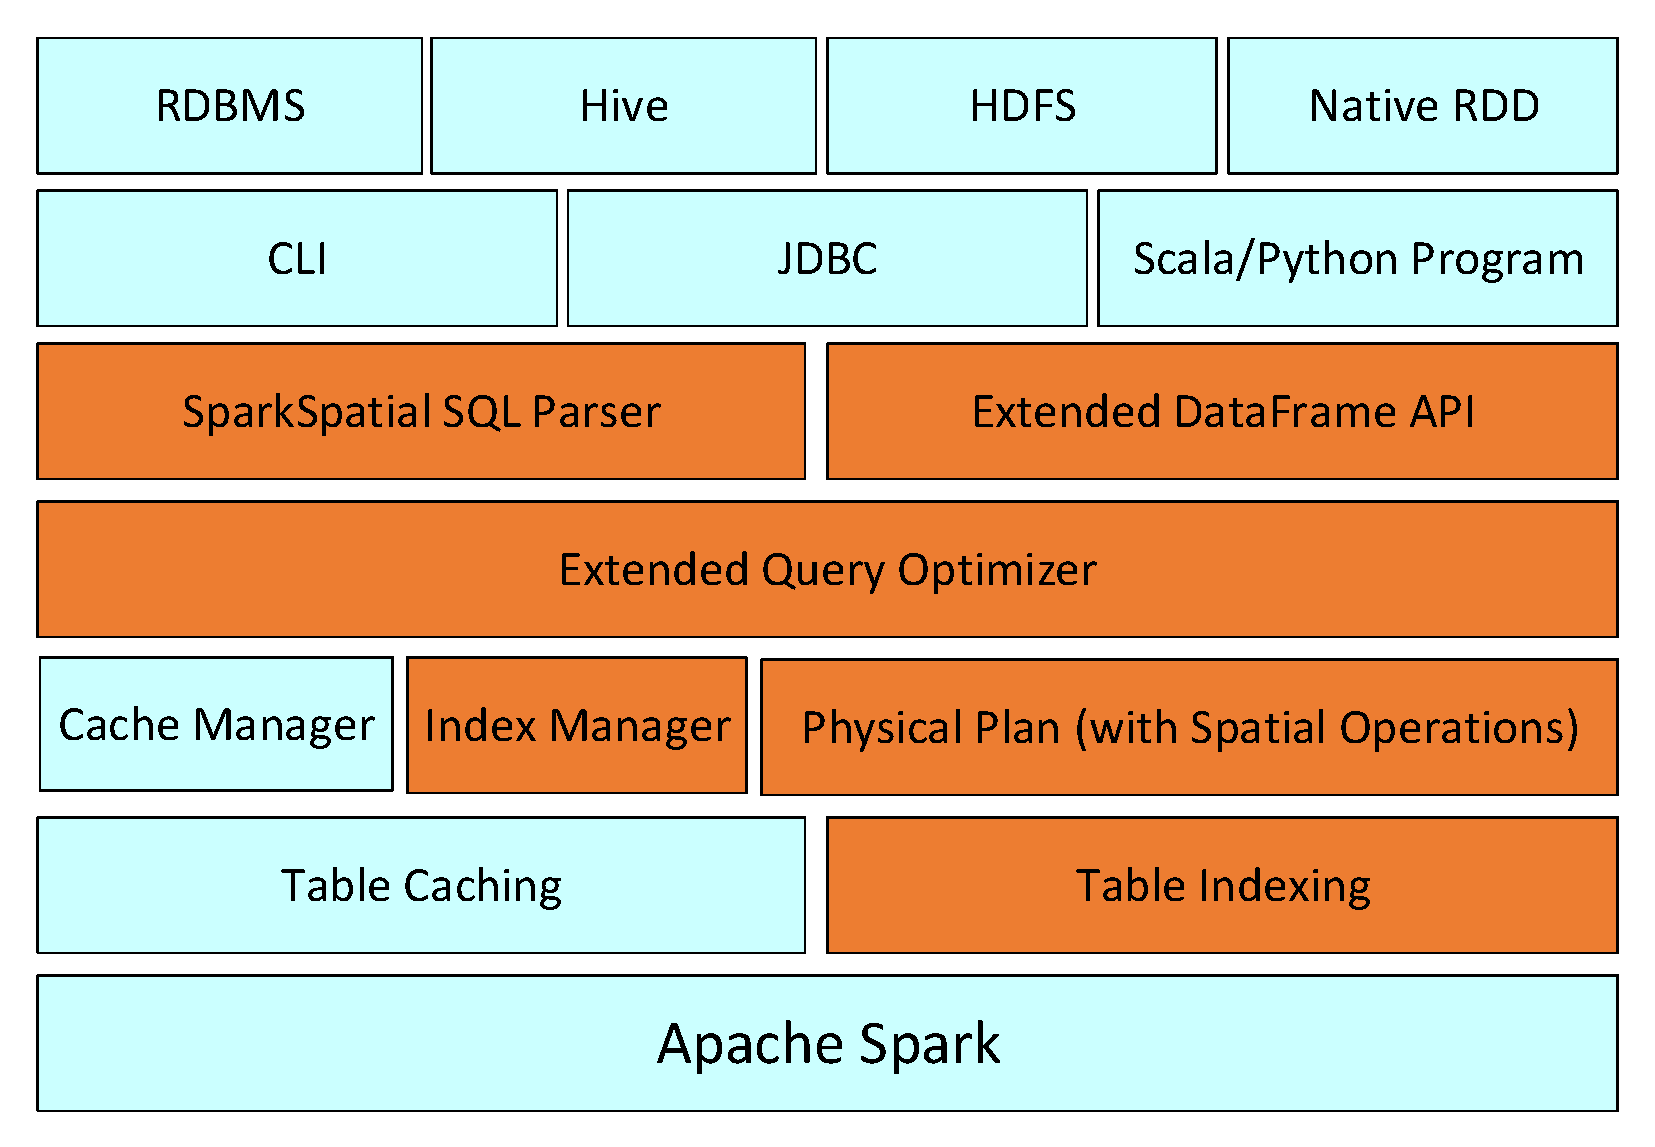
\includegraphics[width = 3.2in]{figs/architecture}
	\vspace{-4mm}
	\caption{\name architecture.}
	\label{fig:architecture}
	\vspace{-4mm}
\end{figure}

\Paragraph{Programming interface.} \name adds spatial
keywords and grammar (e.g. \texttt{POINT}, \texttt{RANGE},
\texttt{KNN}, \texttt{KNN JOIN}, \texttt{DISTANCE JOIN}) in Spark
SQL's query parser, so that user can express spatial queries and
spatial analytical logic in an SQL-like expression. We also extend the
DataFrame API in Spark SQL with similar set of spatial operations,
providing an alternative programming interface for the end user. The
support of spatial operations in the DataFrame API also allows \name
to interchange and interact with other Spark systems easily, such as
SparkML, GraphX, and Spark Streaming. Lastly, we introduce indexing
management to \name's programming interface, in a way that's similar
to that in traditional RDBMS. We will describe the \name's query
interface in details in Section \ref{sec:parser}, and in Appendix
\ref{sec:fullquery}.

\Paragraph{Indexing.} Spatial queries are expensive to process,
especially for data in multi-dimensional space and complex operators
like spatial joins and $\knn$. To achieve efficient and scalable query
performance, \name introduces the concept of {\em indexing} into its
kernel. In particular, \name implements the classic R-tree index
\cite{rtree,DBLP:conf/sigmod/BeckmannKSS90} over the RDD structures in
Spark. \name adopts a two-level indexing strategy: \emph{local} and
\emph{global} indexing. The global index collects statistics from each
RDD partition and helps the system prune irrelevant partitions. Inside
each RDD partition, local indexes are built to accelerate local query
processing, so that linear scan over the entire partition can be
avoided. In \name, user can build and drop indexes anytime on
any table through simple programming interface. Through a construction
called {\em IndexedRDD} which extends the standard RDD structure in
Spark, indexes over RDDs can also be made persistent to disk, and
loaded back, together with associated RDDs, in memory easily. We will
describe the \name's indexing support in Section \ref{sec:index}.

\Paragraph{Spatial operations.} \name supports a number of popular
spatial operations over point and rectangular objects. These spatial
operations are implemented based on the native Spark RDD API. Multiple
access and evaluation paths are provided for each operation, so that
the end users and the \name's query optimizer have the freedom and
opportunities to choose the most appropriate method for a spatial
query or analytical job. Section \ref{sec:query} discusses how various
spatial operations are supported in \name.

\Paragraph{Optimization.} \name extends the logical optimization in
Spark SQL and also introduces a cost-based optimization (CBO) module
that tailors towards optimizing spatial queries. The CBO module
leverages the indexing support in \name, and is able to optimize
complex spatial queries automatically to make the best use of existing
indexes and statistics for the underlying data. Query optimization for
\name is presented in Section \ref{sec:opt}.

\begin{figure}[t!]
  \hspace*{-8mm}
	\centering
	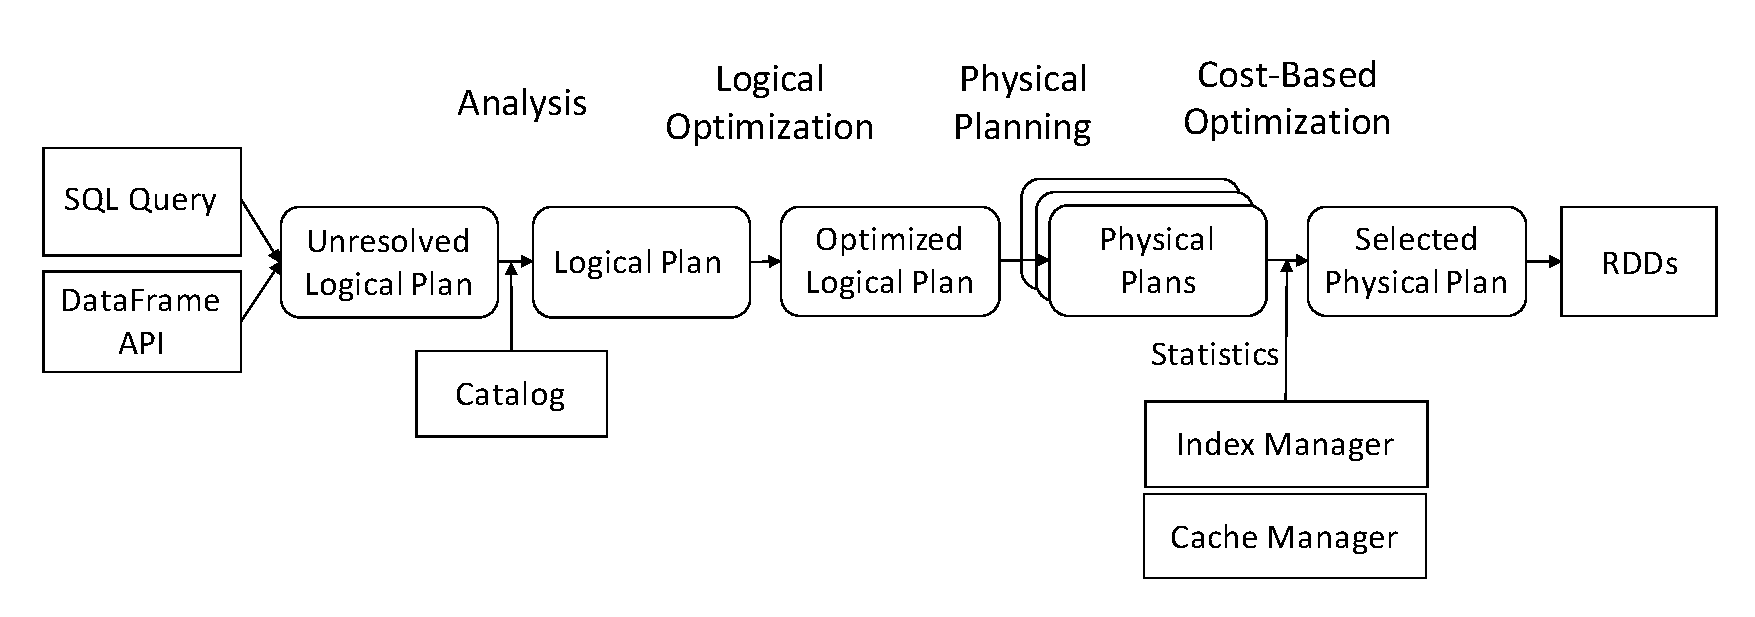
\includegraphics[width = 3.8in]{figs/pipeline}
	\vspace{-8mm}
	\caption{Query processing pipeline in \name.}
	\label{fig:pipeline}
	\vspace{-4mm}
\end{figure}

\Paragraph{Workflow in \name.} Figure \ref{fig:pipeline} shows the
query processing pipeline of \name. \name begins with a relation to be
processed, either from an abstract syntax tree (AST) returned by the
SQL parser or a DataFrame object constructed using the DataFrame
API. In both cases, the relation may contain unresolved attribute
references or relations. An attribute is called {\em unresolved if we
  do not know its type or have not matched it to an input
  table}. \name resolves these attributes with catalyst rules and a
\texttt{Catalog} object that tracks tables in all data sources to
build logical plans. Then, the logical optimizer applies standard
rule-based optimization, such as constant folding, predicate pushdown,
projection pruning, and spatial-specific optimizations such as
distance pruning, to the logical plan. In the physical planing phase,
\name takes a logical plan as input and generates one or more physical
plans based on the spatial operations supported by \name, as well as
using physical operators implemented within Spark's execution
engine. It then applies a cost-based optimizer based on {\em
  statistics collected in both Cache Manager and Index Manager} to
select the most efficient plan.  The physical planner also performs
rule-based physical optimization, such as pipelining projections or
combining filters into one Spark \texttt{map} operation. In addition,
it can push operations from the logical plan into data sources that
support predicate or projection pushdown.

\name supports analytical jobs on various data sources such as CVS,
JSON and JDBC. Figure \ref{fig:storage} shows how data are represented
in \name.  Generally speaking, each data source will be transformed to
an RDD of records (i.e., \texttt{RDD[Row]}) for further
evaluation. \name allows users to materialize (often referred as
``cache'') hot data in memory using columnar storage, which can reduce
memory footprint by an order of magnitude because it relies on Spark
SQL to apply columnar compression schemes such as dictionary encoding
and run-length encoding. Besides, user can build various indexes
(e.g. hash maps, tree maps, R-trees) over different datasets to
accelerate interactive query processing.

%%% Local Variables:
%%% mode: latex
%%% TeX-master: "paper"
%%% End:

\vspace{-2mm}
\section{Programming Interface}
\label{sec:parser}
Spark SQL provides two programming interfaces, the SQL-like relational
query language and the DataFrame API \cite{sparksql}, so that users
can easily express their analytical queries and integrate with other
systems in the Spark ecosystem. \name extends both of the interfaces
to support spatial queries and analytics. We first discuss the
extensions made to the SQL query language in \name.


\begin{figure}[t!]
	\centering
	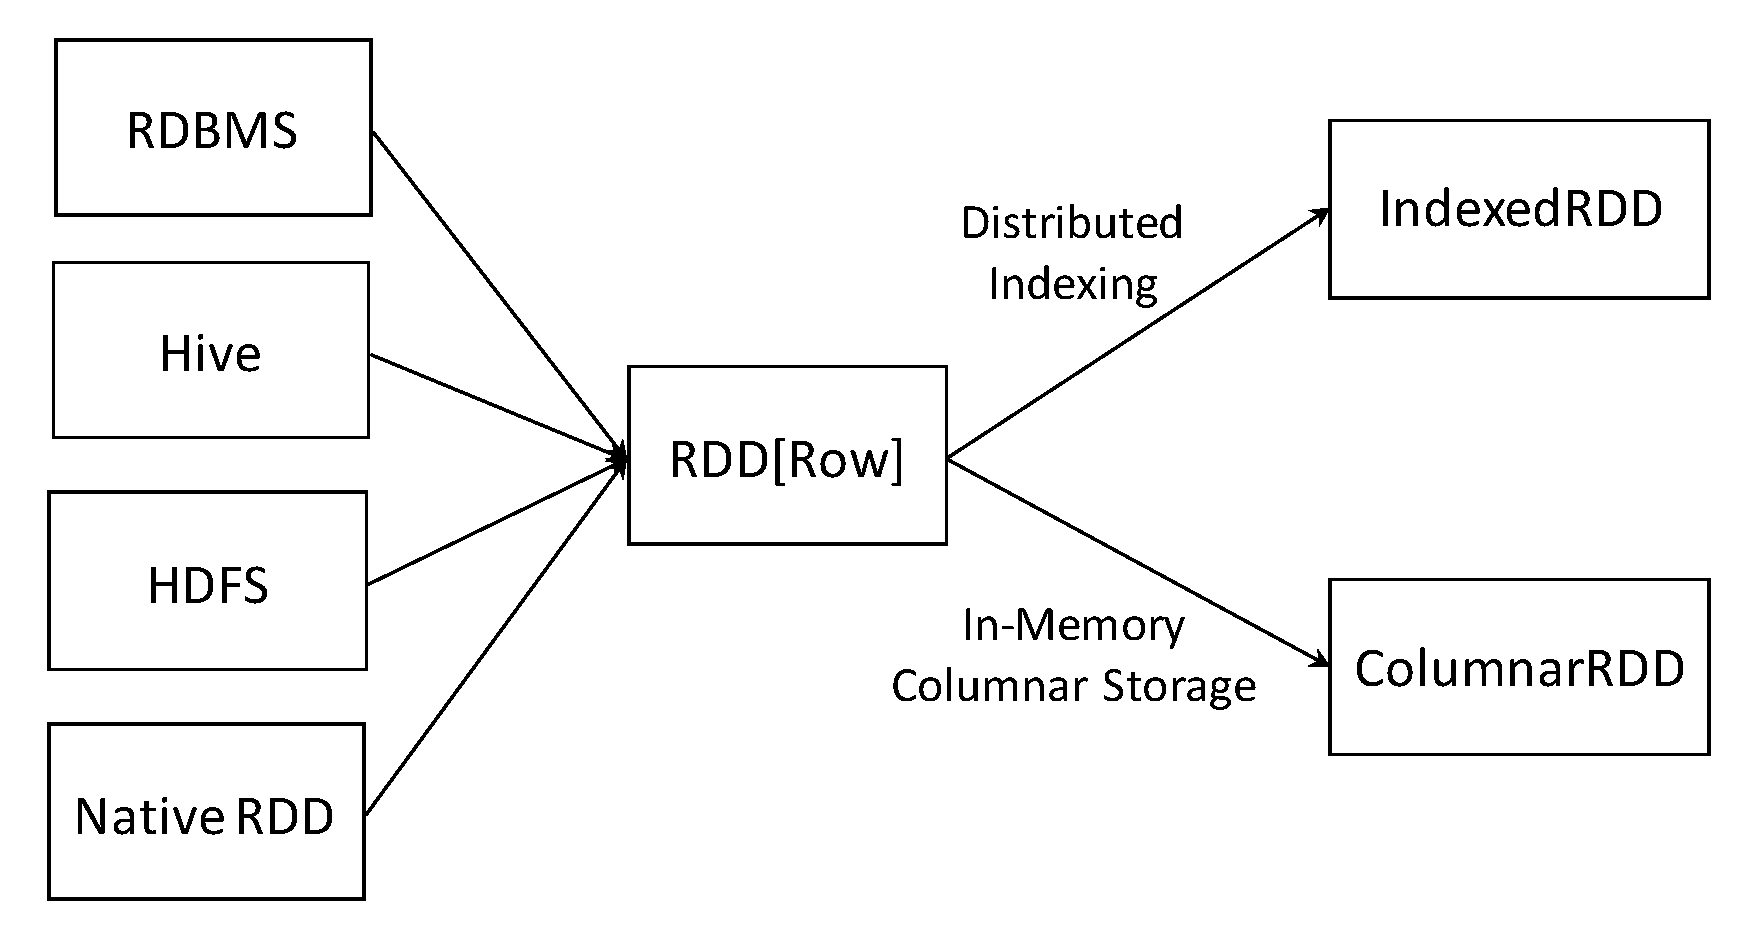
\includegraphics[width = 3.2in]{figs/storage}
	\vspace{-3mm}
	\caption{Data Representation in \name.}
	\label{fig:storage}
	\vspace{-3mm}
\end{figure}



\Paragraph{Points.} Users can express a multi-dimensional point with
the keyword \texttt{POINT}. Not only constants or attributes of
tables, but also arbitrary arithmetic expressions can be used as the
coordinates of points. For example, users can use \texttt{POINT(x + 2,
  y - 3, z * 2)} to express a three dimensional point with the first
coordinate being the addition of attribute \texttt{x}'s value and
constant 2. This offers a flexible way to express spatial points in
the SQL query language. In \name, we will calculate each expression
in the statement and wrap them as a point object for further processing.

\Paragraph{Spatial predicates.} \name adds several new predicates to
SQL to support spatial queries, such as \texttt{RANGE} for box range
queries, \texttt{CIRCLERANGE} for circle range queries with a radius,
and \texttt{KNN} for $k$ nearest neighbor queries. For instance, users
can ask for the 3-nearest neighbors of point $(4, 5)$ from table
\texttt{point1} as below:
\begin{lstlisting}[language=SQL]
SELECT * FROM point1
WHERE POINT(x, y) IN KNN(POINT(4, 5), 3).
\end{lstlisting}\vspace{-2mm}

And a box range query as below asks for all points from table
\texttt{point2} in the 2 dimensional rectangle defined by point
$(10, 5)$ (lower left corner) and $(15, 8)$ (top right corner):
\begin{lstlisting}[language=SQL]
SELECT * FROM point2
WHERE POINT(x, y) IN RANGE(POINT(10, 5), POINT(15, 8)).
\end{lstlisting}\vspace{-1mm}

\Paragraph{Spatial joins.} \name supports two types of spatial joins:
distance joins and $k$NN joins.  Users can express these spatial joins
in a $\theta$-join like manner. Specifically, a 10-nearest neighbor
join between two tables, \texttt{point1} and \texttt{point2}, can be
expressed as:
\begin{lstlisting}[language=SQL]
SELECT *
FROM point1 AS p1 KNN JOIN point2 AS p2
ON POINT(p2.x, p2.y) IN KNN(POINT(p1.x, p1.y), 10).
\end{lstlisting}\vspace{-2mm}

A distance join with a distance threshold $20$, between two tables
\texttt{point3} and \texttt{point4} in 3 dimensional space, is
expressed as:
\begin{lstlisting}[language=SQL]
SELECT *
FROM point3 AS p3 DISTANCE JOIN point4 AS p4
ON POINT(p4.x, p4.y, p4.z) IN CIRCLERANGE(POINT(p3.x, p3.y, p3.z), 20).
\end{lstlisting}\vspace{-2mm}



\Paragraph{Indexing command.} Users can manipulate indexes in \name
easily with indexing commands introduced by \name. For example, users
can build an R-Tree index called \texttt{pointIndex} on attributes
\texttt{x}, \texttt{y}, and \texttt{z} for table \texttt{sensor} using
command:
\begin{lstlisting}[language=SQL]
CREATE INDEX pointIndex ON sensor(x, y, z) USE RTREE.
\end{lstlisting}\vspace{-2mm}

\Paragraph{Complex queries.} Note that \name has kept the support for
all grammars (including UDFs and UDTs) supported by Spark SQL. As a
result, we can express complex spatial queries in a single SQL
statement. For example, we can count the number of restaurants near
(say within distance 10) a POI for a set of POIs, and sort
locations by the counts, with the following query:
\begin{lstlisting}[language=SQL]
SELECT q.id, count(*) AS c
FROM pois AS q DISTANCE JOIN rests AS r
ON POINT(r.x, r.y) IN CIRCLERANGE(POINT(q.x, q.y), 10.0)
GROUP BY q.id
ORDER BY c.
\end{lstlisting}\vspace{-2mm}

\Paragraph{DataFrame support.} Besides SQL, user can also perform
spatial operations on DataFrames using a domain-specific language
(DSL) similar to R data frames. \name's DataFrame API supports all
spatial operations extended to the SQL query language described
above. Naturally, all new operations are also compatible with the
exiting ones from R and Spark SQL, which provides the same level
flexibility as \name's SQL does. For instance, we can also the last
SQL query above in the following scala code:
%including range queries (\texttt{range}), $k$ nearest neighbors (\texttt{knn}), distance joins (\texttt{distanceJoin}) and $k$NN joins (\texttt{knnJoin}).
\begin{lstlisting}
pois.
  .distanceJoin(rests, Point(pois("x"), pois("y")),
                       Point(rest("x"), rest("y")), 10.0)
  .groupBy(pois("id"))
  .agg(count("*").as("c")).sort("c").show().
\end{lstlisting}

%%% Local Variables:
%%% mode: latex
%%% TeX-master: "paper"
%%% End:

\vspace{-2mm}
\section{Indexing}
\label{sec:index}
Indexing is important for the efficient processing of spatial queries
and analytics, especially for multi-dimensional spatial data and
complex spatial queries such as $\knn$ and spatial joins. In
particular, indexing is a critical component towards building an
effective optimizer in \name. Since \name is an in-memory analytical
engine, hence, reducing disk IOs is not a main focus of
indexing. Rather, the main objective of indexing in \name is to reduce
query latency via reducing cpu costs, and improve the over query
throughput in the system. For example, indexing helps prune irrelevant
RDD partitions (to an input query) which frees more cpu resources for
the underlying Spark engine, leading to higher query
throughput. Spatial indexing also helps speed up query processing for
complex queries such as $\knn$ and spatial joins. For example, Spark
and Spark SQL have to execute a $\knn$ join through cartesian product
between two (RDD) tables which is very expensive and not scalable,
whereas \name is able to process a $\knn$ join through distributed
R-tree index over the RDDs and dramatically reduce the query latency.

% Spark SQL claims that indexing is less important due to its in-memory
% computational model. However, it is not true when dealing with
% multi-dimensional data. For example, to process a $k$NN query, we need
% to calculate distances from the query point to all data points, take
% $k$ points with minimum distances in each partition and merge them in
% the driver program when processing without indexes. Such procedure
% requires touching every record in the table, thus will take numerous
% computing resources in the cluster. In contrast, if we have indexes
% built on tables, we can leverage them to cut down useless computations
% and improve system performance.

\name builds spatial indexes directly on RDDs to help speed up query
processing.  In Spark SQL, tables are represented as RDDs of records
(i.e., \texttt{RDD[row]}). Hence, indexing records of a table becomes
the problem of indexing elements in an RDD. However, RDDs are designed
for sequential scan, and random access is not supported and is very
expensive as it may simply become a full scan on the RDD. An added
complexity is that we want to introduce indexing support {\em without
  changing the Spark core} for the reasons explained in Section
\ref{sec:overview}. To overcome these challenges, we change the
storage format for an indexed table, i.e., a new abstraction called
\texttt{IndexedRDD[row]}, and employ a two-level indexing
strategy. This indexing strategy can accommodate different index
structures to support different queries in \name.


\Paragraph{IndexedRDD.} Records from a table in Spark SQL are stored
as \texttt{Row} objects and tables are stored as RDDs of \texttt{Row},
hence a table is stored as \texttt{RDD[row]} which may have many
partitions. To add index support over these records, we pack all
records (i.e. \texttt{Row} objects) within a RDD partition into an
array, which gives each record an unique subscript as its index. This
change also makes random access inside a RDD partition an efficient
operation with $O(1)$ cost. In particular, we introduce the
\texttt{IPartition} data structure:

\begin{lstlisting}[language=java]
case class IPartition[Type](Data: Array[Type], I: Index),
\end{lstlisting}\vspace{-1mm}
where \texttt{Index} is an abstract scala class we have designed and
it is instantiated with the following implementations:
\texttt{HashMap} (a hash index), \texttt{TreeMap} (a one dimension
index), and \texttt{RTree} (a multi-dimension index). Finally,
\texttt{IndexedRDD[Row]} is defined as \texttt{RDD[IPartition[Row]]},
when setting \texttt{Type=Row}:
\begin{lstlisting}[language=java]
type IndexedRDD[Type] = RDD[IPartition[Type]],
\end{lstlisting}\vspace{-1mm}
where the set of records from a table is partitioned into a set of
IPartition objects through the {\em partitioner} that will be
described next.

Each IPartition object represents a {\em local index} over records in
that partition. Furthermore, each IPartition object emits the
partition boundary information to construct a {\em global index}. That
being said, index construction in \name consists of three phases:
\emph{partition}, \emph{local index}, and \emph{global index}, as
shown in Figure \ref{fig:index}.

\begin{figure}[t!]
	\centering
	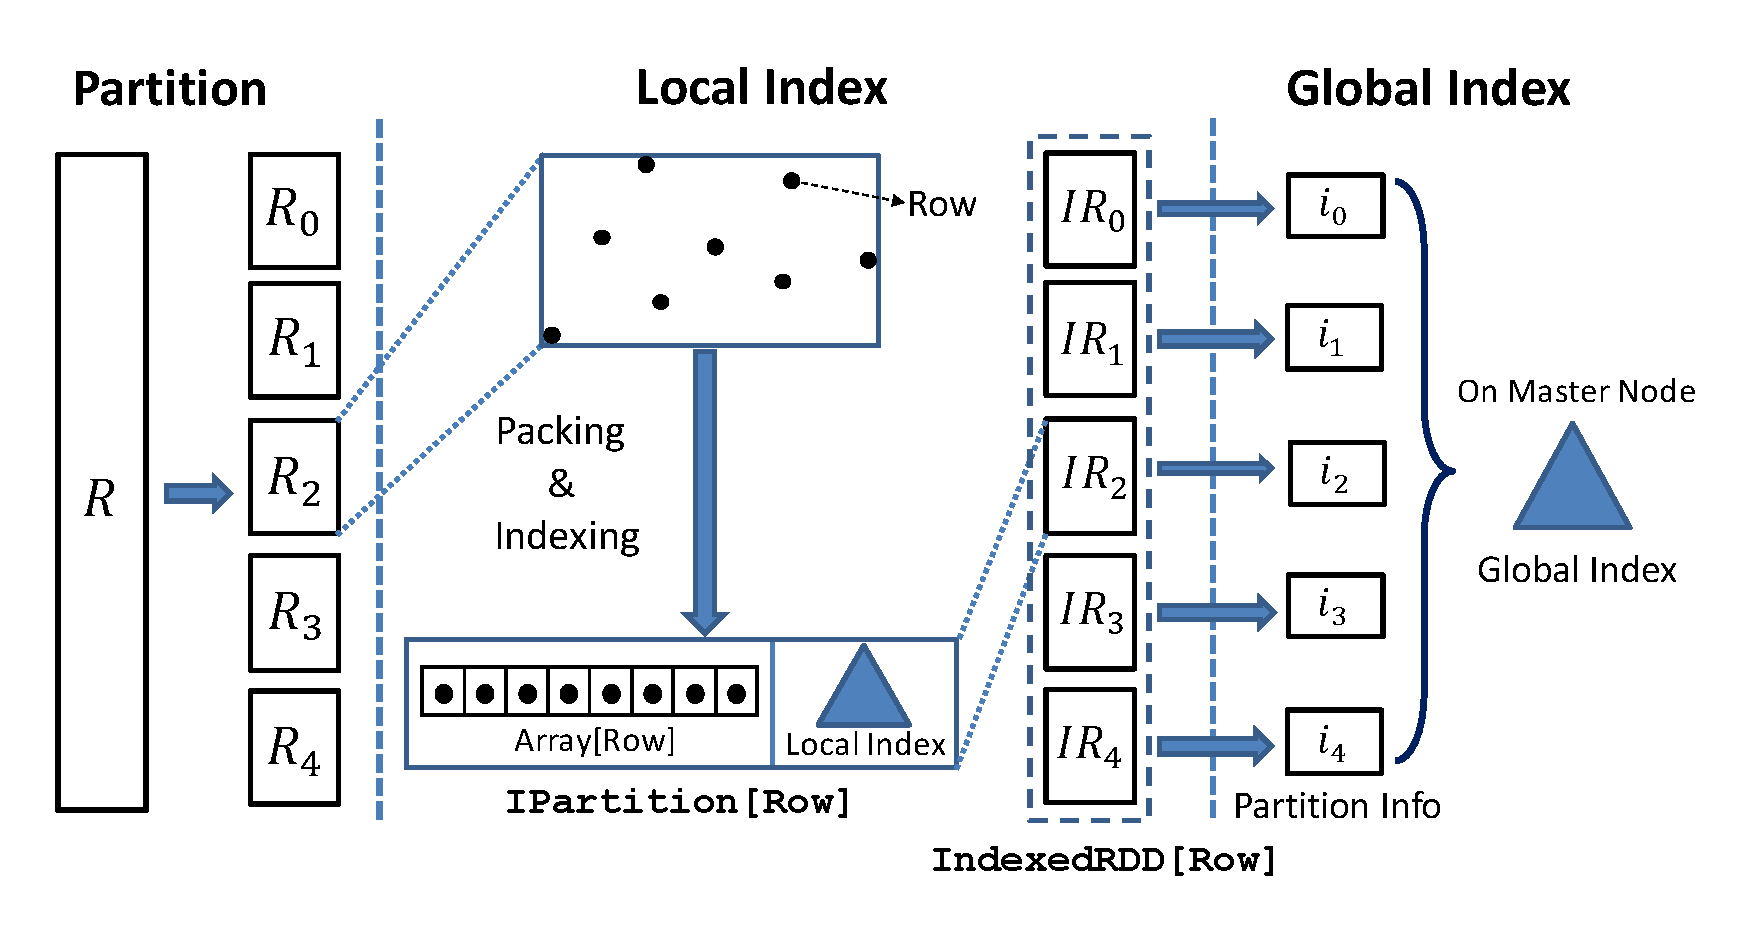
\includegraphics[width=3.4in]{figs/index}
	\vspace{-8mm}
	\caption{Two-level indexing strategy in \name.}
	\label{fig:index}
    \vspace{-4mm}
\end{figure}


\Paragraph{Partition.} The partition phase uses a {\em partitioner} to
partition a table of input data. The partitioner is an abstract class
that can be instantiated with different implementations on the
following key modules: (1) \emph{Partition Size.} Each partition
should have a proper size so as to avoid memory overflow. (2)
\emph{Data Locality.}  Records that locate close to each other (with
respect to the indexing attributes) should be assigned to the same
partition. (3) \emph{Load Balancing.} Partitions should be roughly of
the same size.

Spark allows users to define the partition strategy by implementing an
abstract class called \texttt{Partitioner}. A customized partitioner
should specify how many partitions it will generate and how an element
map to a according to its partition key. Spark provides two predefined
partitioners, range partitioner and hash partitioner, which is
sufficient when the partition key is one dimensional, but does not fit
well to the multi-dimensional case.

To address this problem, we defined a new partitioner named
\texttt{STRPartitioner} in \name. \texttt{STRPartitioner} takes a set
of random samples from the RDD for the input table and runs the first
iteration of Sort-Tile-Recursive (STR) algorithm \cite{str} to
determine partition boundaries. Note that boundaries generated by the
STR algorithm are minimum bounded rectangles (MBRs) of the samples,
thus, we need to extend theses MBRs so that they can properly cover
the space of the original data set. Finally, according to these
extended boundaries, \texttt{STRPartitioner} specifies the partition
that each record belongs to.

Note that \name makes no restriction as what partition strategy users
want to use. Instead of using the \texttt{STRPartitioner}, the end
user can always supply his/her own partitioner to \name. We choose the
\texttt{STRPartitioner} as the default partitioner in \name due to its
simplicity and proven effectiveness by many existing studies. As shown
in Figure \ref{fig:index}, we assume a RDD for an input table $R$ is
partitioned into a set of partitions $\{R_1, \ldots, R_m\}$ by the
partitioner. The number of partitions, $m$, is determined by \name's
optimizer which is discussed in Section \ref{sec:opt}.

\Paragraph{Local index.} In this phase, \name builds a user-specified
index structure, e.g., \texttt{RTree}, as a \emph{local} index for
data in each partition $R_i$ for $i\in\{1, \ldots, m\}$. Meanwhile, we
also alter the storage format of the input RDD from \texttt{RDD[Row]}
to \texttt{IndexedRDD[Row]}, by converting the RDD partition (a
partition of RDD[Row]) for each partition $R_i$ to an IPartition[Row]
object, as show in Figure \ref{fig:index}. In particular, records in
$R_i$ are stored into the \texttt{Array[Row]} object in the
\texttt{IPartition[Row]} object for $R_i$.

The \emph{local} index is built over the \texttt{Array[Row]} object
for each partition , and is co-located with \texttt{Array[Row]} object
within an \texttt{IPartition[Row]} object. The local index and the
local data from the partition's array of rows form the
\texttt{IPartition[Row]} object. As we can see, the storage format of
a table is no longer an RDD of \texttt{Row} objects, but an RDD of
\texttt{IPartition[Row]} objects, which by the definition above is an
\texttt{IndexedRDD} of \texttt{Row} objects. While packing partition
data and building local indexes, \name also collects several
statistics from each partition, such as number of records and
partition boundary, to facilitate the construction of the global
indexing as illustrated in Figure \ref{fig:index}.

Local indexes can be easily made persistent and fault tolerant, by
persisting the \texttt{IndexedRDD} (which is still a RDD object!) at
the \texttt{MEMORY\_AND\_DISK\_SER} storage level in Spark. This also
allows local indexes to be reused when data are loaded back into
memory from disk again, and avoids the rebuilding of partitions and
local indexes.

% By now, we finish local indexing for each partition and change
% storage format of the table from \texttt{RDD[Row]} to
% \texttt{RDD[PackedPartitionWithIndex]}.

\Paragraph{Global index.} The last phase of index construction is to
build a \emph{global} index which indexes all partitions. The global
index enables us to prune irrelevant partitions for an input query
{\em without invoking many workers} to look at data stored in
different partitions.

In this phase, partition boundaries generated by the partitioner and
other statistics collected in the local index phase are sent to the
{\em master node}. The master node utilizes these information to bulk
load an in-memory index which is stored in the {\em driver
  program}. Users may specify different types of global index. When
indexing one-dimensional data, a sorted array for the one dimensional
range boundaries is sufficient (the record count and other statistics
for each partition are also stored in each array element). In
multi-dimensional case, more complex index structures, such as R-Tree
\cite{rtree,DBLP:conf/sigmod/BeckmannKSS90} or KD-tree, which indexes
the MBRs for all partitions can be used. By default, \name keeps the
global indexes for different tables in the memory of the master node
at all time (i.e., in its driver program). But \name also allows users
to choose to persist the global indexes, and the corresponding
partition information and statistics to the file system.

\Paragraph{Fault tolerance.} By its construction, local indexes and
data in \name are {\em persisted automatically by the RDD abstraction
  of the Spark system}. Global indexes are kept in the heap space of
the driver program on the master node with no fault tolerance
guarantees by Spark. Nevertheless, global indexes can be lazily
reconstructed from partition boundaries and statistics collected from
persisted RDD when required, and as mentioned above, users can also
choose to persist them and then have the option of loading them back
from the file system.


%%% Local Variables:
%%% mode: latex
%%% TeX-master: "paper"
%%% End:

\section{Spatial Operations}
\label{sec:query}
\name introduces new {\em physical execution plans} inside Spark SQL
for spatial operations. In particular, the support for local and
global indexes enables \name to explore many efficient implementations
of classic spatial operations in the context of Spark. In this
section, we will discuss four operators as representatives for spatial
queries and analytics in \name, namely, range query, k nearest
neighbor ($\knn$) query, distance join, and $\knn$ join.

\subsection{Range Query}
\label{sub:range}
Two types of range queries are supported in \name. They differ by the
shape used to specify the query area, which is either a rectangular
box or a circle, leading to box and circle range query
respectively. Intuitively, these range queries can be expressed and
treated as standard SQL queries in Spark SQL, using filters with
properly constructed range conditions. However, without using \name's
query interface introduced in Section \ref{sec:parser}, the expression
becomes clumsy and error prone. And more importantly, without indexes,
the query evaluation will have to scan all records in the table, which
is very inefficient and resource intensive.

In contrast, \name allows users to express both range queries
natively as shown in Section \ref{sec:parser}, and it can handle range
queries using index (assume that the spatial attributes are indexed):

% \begin{figure}[t!]
% 	\centering
% 	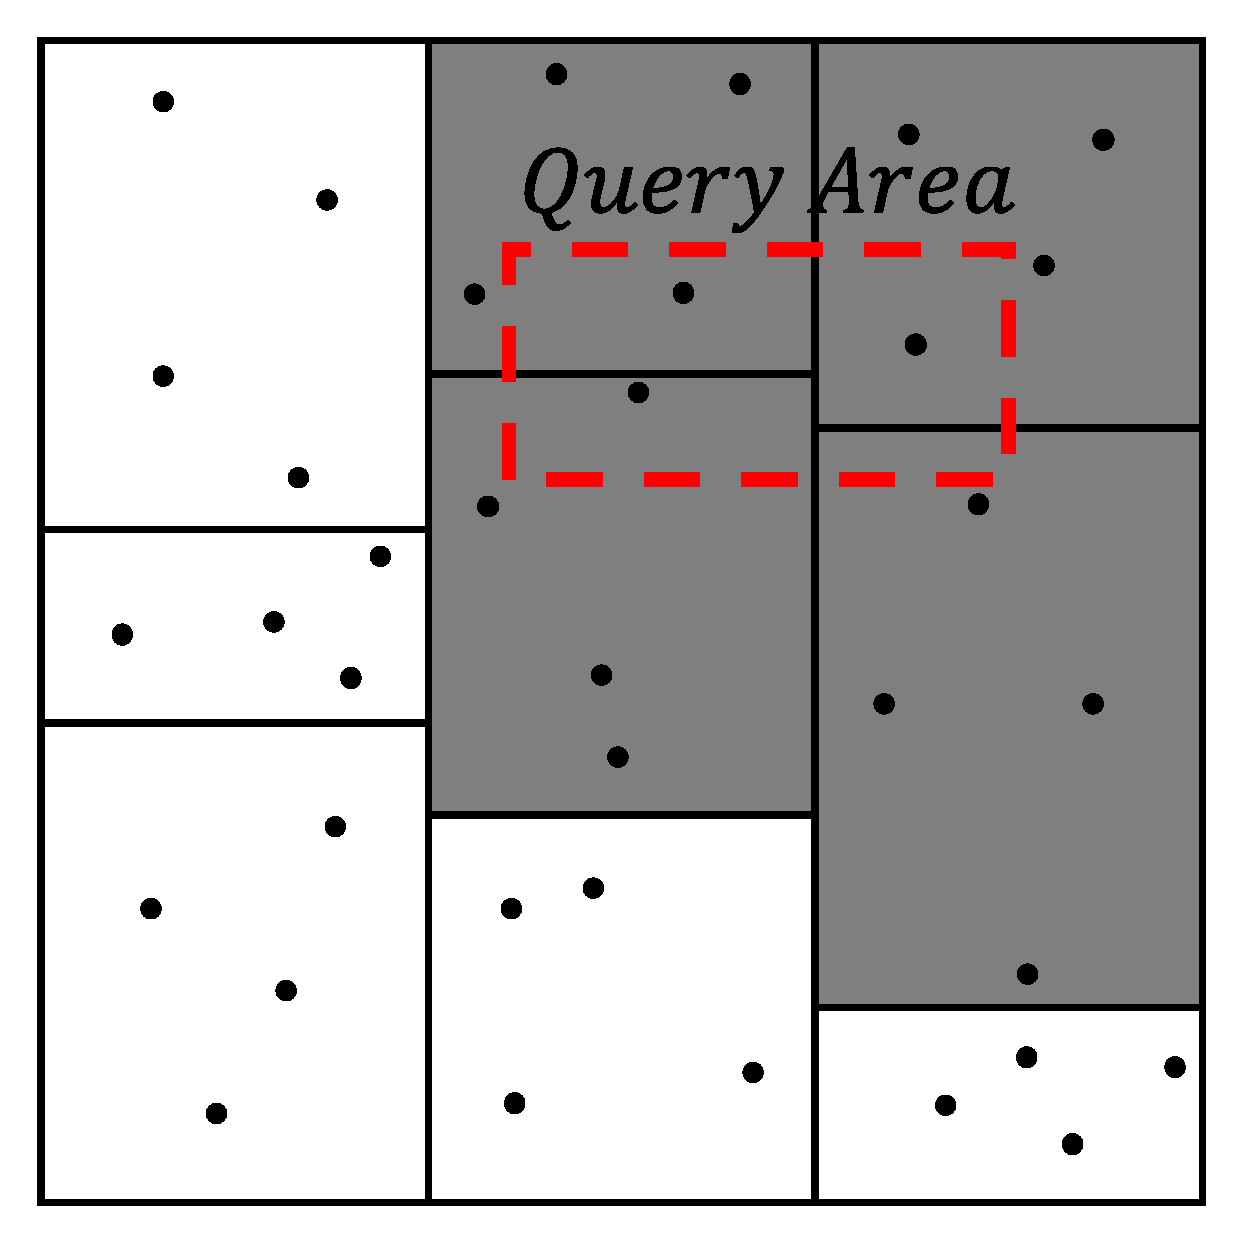
\includegraphics[width = 1.55in]{figs/range}
% 	\vspace{-4mm}
% 	\caption{Range Query}
% 	\label{fig:oprange}
%     \vspace{-3mm}
% \end{figure}


\Paragraph{Global filtering.} In this step, \name uses the global
index to prune partitions that do not overlap with the query range. In
particular, \name inspects the global index to obtain ids of the
partitions which intersect the query area. Next, \name calls
\texttt{PartitionPruningRDD}, a Spark internal developer API that
filters partitions by ID, to mark required partitions.

\Paragraph{Local processing.} On selected partitions from global
filtering, \name processes them in parallel. For each partition, \name
exploits its local index to quickly return matching records from the
local array. Note that if $\mbr(R_i)$ is completely inside the query
area, all records in $R_i$ can be returned without even checking the
index. In general, local index helps reduce query cost over $R_i$
significantly compared to scanning $R_i$ entirely in Spark SQL.

% For instance, in Figure \ref{fig:oprange}, we first query the global
% index to find all partitions whose regions intersect the query area
% (shaded area in the figure). Then, \SparkSpatial invokes a range query
% on the local index of each selected partitions to get the final
% results.
\subsection{kNN Query}
\label{sub:knn}
Using Spark SQL, a $k$NN query can be processed in two steps: (1)
calculate distances from all points in the table to the query point;
(2) take $k$ records with minimum distances. This procedure can be
naturally expressed as an RDD action \texttt{takeOrdered}, where users
can specify a comparison function and a value $k$ to select $k$
minimum elements from RDD. However, this solution invokes distance
computation for every record, a top $k$ selection on each RDD
partition, and shuffling of large intermediate results.

In \name, $k$NN queries achieve much better performance by utilizing
indexes. It leverages two observations: (1) once at a local partition,
fast $k$NN selection over the local data is possible using the local
index; (2) a tight pruning bound that is sufficient to cover the
global $k$NN results can be used for pruning at the global index. The
first observation is a simple application of classic $k$NN query
algorithms using spatial index like R-tree
\cite{DBLP:conf/sigmod/RoussopoulosKV95}. The second observation
deserves some discussion.
\begin{figure}[htb]
	\subfigure[Loose Pruning Bound]{
		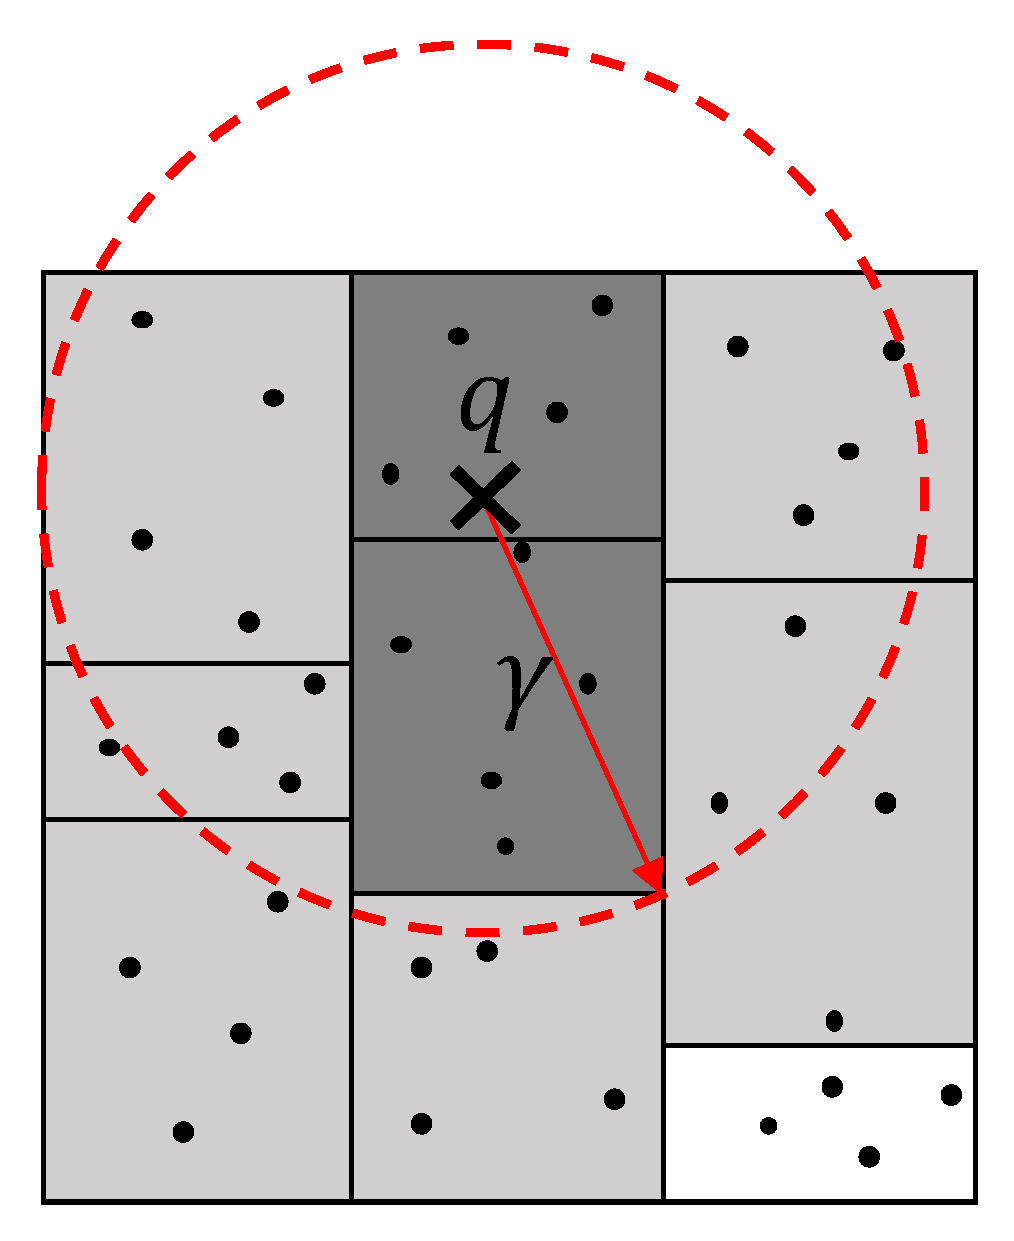
\includegraphics[width=1.55in]{figs/knnbound1}
		\label{fig:knnbound1}}
	\subfigure[Refined Pruning Bound]{
		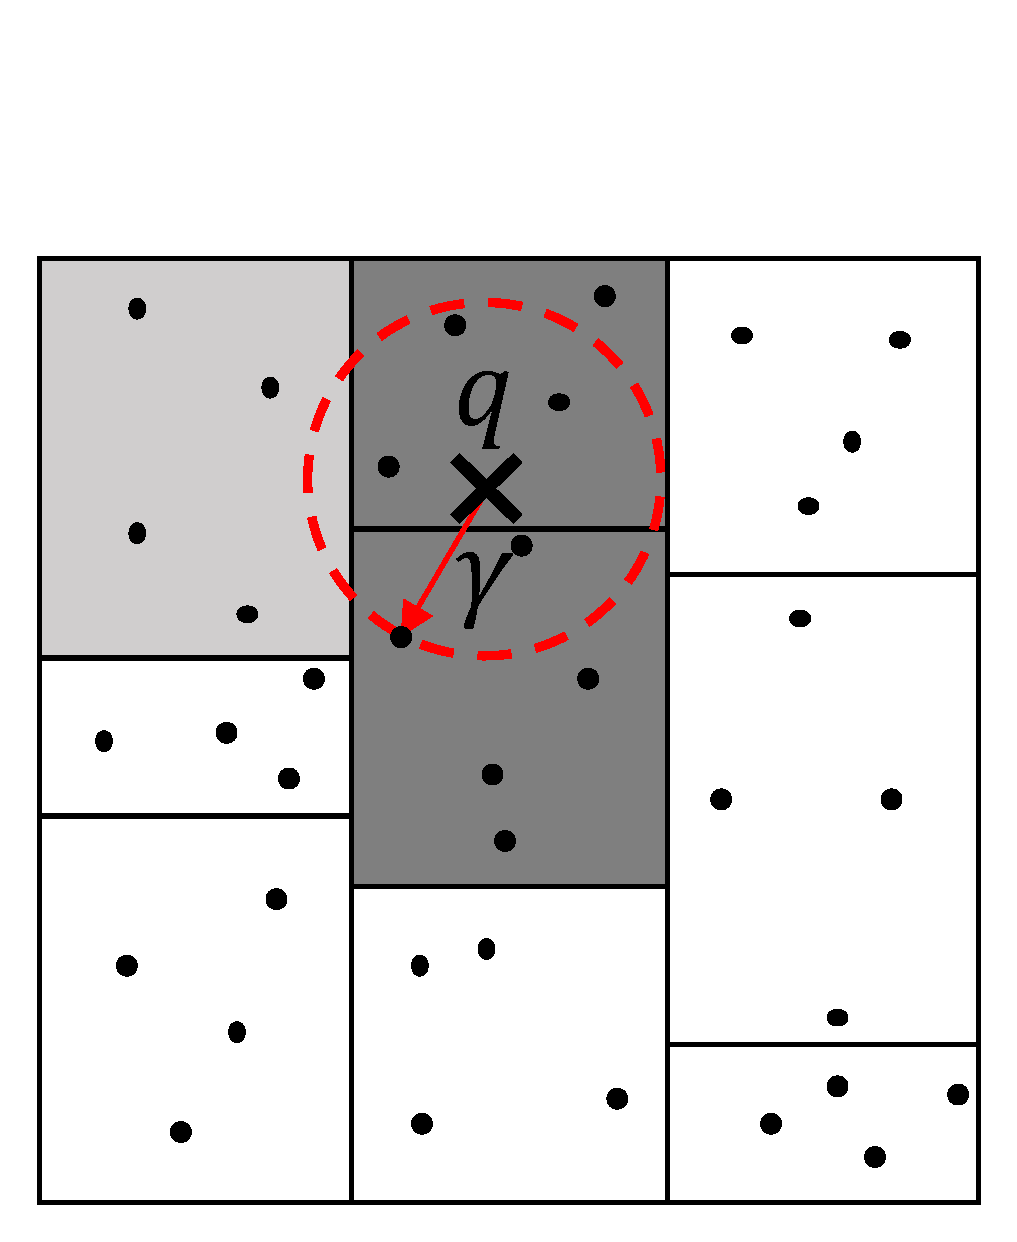
\includegraphics[width=1.55in]{figs/knnbound2}
		\label{fig:knnbound2}}
	\caption{Pruning bound for $k$NN query at global index.}%\vspace{-1mm}
	\label{fig:knnbound}
\end{figure}

Intuitively, any circle that centers at the query point $q$ and covers
at least $k$ points from $R$ is a safe bound for pruning. To generate
a tight pruning bound, we need to shrink the radius $\gamma$ of this
circle. A loose pruning bound can be obtained using the global index.
We find the nearest partition(s) to the query point $q$, that are
sufficient to cover at least $k$ data points; retrieve more than one
partitions if the nearest partition does not have $k$ points (note
that global index maintains the counts for the number of records in
each partition). The distance between $q$ and a partition $R_i$ is
defined as $\maxdist(q, \mbr(R_i))$
\cite{DBLP:conf/sigmod/RoussopoulosKV95}. Without loss of generality,
assume the following MBRs are returned:
$\{\mbr(R_1), \ldots, \mbr(R_\ell)\}$.  Clearly,
$\gamma=\max\{\maxdist(q, \mbr(R_1)), \ldots, \maxdist(q, R_\ell)\}$
is a safe pruning bound. Figure \ref{fig:knnbound1} shows an example
of this bound as a circle centered at $q$. The dark boxes are the
nearest MBRs retrieved to cover at least $k$ points which help derive
the radius $\gamma$. The dark and gray boxes with shadows are
partitions selected by the global index according to this pruning
bound.

To tighten the pruning bound, \name issues a $k$NN query on the $\ell$
partitions selected from the first step (i.e., two partitions with
dark boxes in Figure \ref{fig:knnbound1}), and takes the $k$-th
minimum distance from $q$ to the $k\ell$ candidates returned from
these partitions as $\gamma$.  Figure \ref{fig:knnbound2} shows this
new pruning bound which will be much tighter in practice. Note that
$\ell$ is small for typical $k$ value (often $\ell=1$), thus, this
step has very little overhead.

Global index returns the partition ids whose MBRs intersect with the
circle centered at $q$ with radius $\gamma$, \name marks these
partitions using \texttt{PartitionPruningRDD} and invokes local $k$NN
queries using the aforementioned observation (1). Finally, it merges
$k$ candidates from each such partition and takes the $k$ records with
minimum distance to $q$ using RDD action \texttt{takeOrdered}.

\subsection{Distance Join}
\label{sub:disjoin}
Distance join is a $\theta$-join between two tables. Hence, we can
express a distance join $R \Join_{10.0} S$ in Spark SQL as:
\begin{lstlisting}[language=SQL]
SELECT * FROM R JOIN S
ON (R.x - S.x) * (R.x - S.x) + (R.y - S.y) * (R.y - S.y)
     <= 10.0 * 10.0
\end{lstlisting}\vspace{-2mm}

Spark SQL will have to use the cartesian product of two input tables
to process $\theta$-joins.  It filters rows from the cartesian product
based on the given predicates. Producing and scanning through
the cartesian product is rather costly in Spark, since it is based on
broadcasting the partitions and if two tables are roughly the same
size, this leads to $O(n^2)$ cost if each table has $n$ partitions.

Note that most existing systems we reviewed in Section
\ref{sec:background} have not studied distance join; rather, they
studied {\em spatial join}. A {\em spatial join} takes two tables $R$
and $S$ (each is a set of spatial objects expressed as some geometric
objects such as polygons), and a spatial join predicate $\theta$
(e.g., \texttt{overlaps}, \texttt{contains}) as input, and it returns
the set of all pairs $(r, s)$ where $r \in R$, $s \in S$ such that
$\theta(r, s)$ is true; $\theta(r,s)$ is evaluated as object $r$
`$\theta$' (e.g, overlaps) object $s$.  

That said, we design the \emph{DJSpark} algorithm in \name for
distance joins.  DJSpark consists of three steps: data partition,
global join, and local join, as shown in Figure \ref{fig:sjmrdis}.

\Paragraph{Data partition.} The main objective of data partition phase
is to partition $R$ and $S$ so that spatial locality is preserved and
records that are close to each other (from both $R$ and $S$) will end
up in the same corresponding partitions. Besides, we also need to
consider partition size (so data from two corresponding partitions
from $R$ and $S$ respectively can both fit in memory) and load
balancing issues. Therefore, we can re-use the \emph{STRPartitioner}
introduced in Section \ref{sec:index} as the partitioner. The main
difference is how we decide the partition size for $R$ and $S$. \name
needs to ensure that it can keep two partitions (one from $R$ and one
from $S$) rather than one (when handling single-relation operations like
range queries) in executors' heap memory space at the same time. 

Note that the data partition phase can be skipped for $R$ (or $S$) if
$R$ (or $S$) is already indexed.

\Paragraph{Global join.} Given the partitions for tables $R$ and $S$,
this step produces all pairs $(i, j)$'s which may contribute any pair
$(r, s)$, such that $r\in R_i$, $s\in S_j$, and $|r, s|\le \tau$.
Observe that each record in $s\in S$, $s$ matches with some records in
$R_i$ {\em only if} $\mindist(s, R_i)\le \tau$. We can generalize to
produce the pairs $(i, j)$'s such that \name only checks them if
$\mindist(R_i, S_j)\le \tau$. After generating these candidate pairs
of partition ids, \name produces a single partition $P=\{R_i, S_j\}$
for each pair $(i, j)$ and these partitions are sent to workers for
processing local joins in parallel.

\Paragraph{Local join.} Given a partition $P=\{R_i, S_j\}$ produced by
the global join, local join builds a local index over $S_j$ on the fly
(if $S$ is not already indexed). For each record $r\in R_i$, \name
finds all $s\in S_j$ such that $|s, r|\le \tau $ using $r$ over the
local index on $S_j$.

\begin{figure}
	\centering
	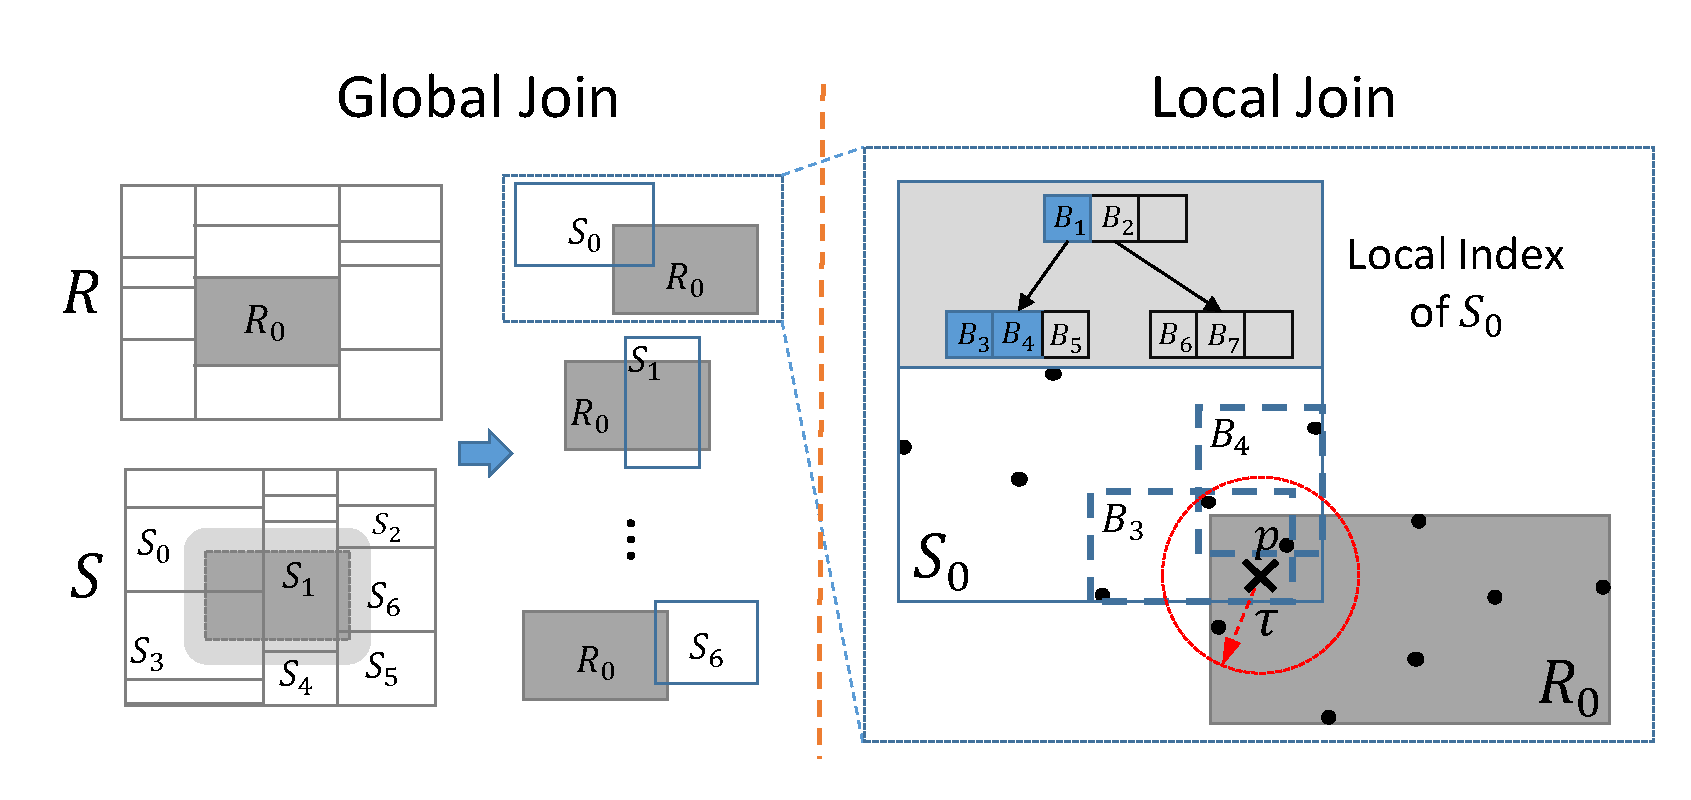
\includegraphics[width = 3.4in]{figs/SJMR-DIS}
	\vspace{-8mm}
	\caption{The DJSpark algorithm in \name.}
	\label{fig:sjmrdis}\vspace{-4mm}
\end{figure}

% For distance joins whose matched record number is not too large,
% \SarkSpatial provides an alternative approach (termed as R-Tree
% distance join) similar to distributed hash join. Instead of finding
% all matched partition pairs in the second step described above, we
% duplicate each record in $S$ as a matching candidate of $P_R^i$ if its
% minimum distance to $A_R^i$ is less than $rd$. To get the final
% result, \SparkSpatial combines $P_R^i$ with all its matching
% candidates in a partition and invokes a local join on each combined
% partition to get the final result. This algorithm avoids data
% partitioning on $S$ and reduces record duplication as duplication
% granularity is on record level rather than partition level. However,
% when $rd$ is getting larger, sizes of the combined partitions will
% grow drastically and finally cause memory overflow.

\subsection{kNN Join}
\label{sub:knnjoin}
Several solutions \cite{bcknnj, feifeiknnj} for $k$NN join have been
proposed in the MapReduce framework. \name has redesigned and
implemented these methods with the RDD abstraction of
Spark. Furthermore, \name designs a new simple hash-join like
algorithm based on the STR partitioning strategy and its R-tree index,
which shows the best performance in Spark. % We will briefly describe
% the the adaption of existing methods into \name, and introduce our new
% algorithm RKJSpark.

\subsubsection{Baseline methods}
\label{subsub:bnlj}
The most straightforward method is to adopt the block nested loop
methodology \cite{feifeiknnj}. We dub this method \emph{BKJSpark-N}
(block nested loop $k$NN join in Spark).

\Paragraph{Producing buckets.} $R$ (and $S$) is divided into $n_1$
($n_2$) equal-sized blocks, which simply puts every $|R|/n_1$ (or
$|S|/n_2$) records into a block. Next, every pair of blocks, i.e.,
$(R_i, S_j)$ for $i\in[1, n_1], j\in [1, n_2]$ are shuffled to a
bucket (so a total of $n_1n_2$ buckets). % \name uses \texttt{flatmap}
% over each record $r$ to assign a bucket number for $r$.  A partitioner
% is implemented to partition RDDs according to these bucket
% numbers. The values of $n_1$ and $n_2$ are determined based on the
% memory size of worker nodes and the size of the input relation.

\Paragraph{Local $k$NN join.} Buckets are processed in
parallel. Within each bucket $(R_i, S_j)$, \name performs
$\knn(r, S_j)$ for every $r\in R_i$ though a nested loop over $R_i$
and $S_j$. % The result for each record
% $r \in R$ is passed to next step in form $(r, list(s, |r, s|))$ where
% the list stores local $k$NN of $r$.

\Paragraph{Merge.} This step finds the global $k$NNs for every
$r \in R$ among its $n_2$ local $k$NNs found in the last step (a total
of $nk$ candidates). \name runs \texttt{reduceByKey} (where key is a
record in $R$) in parallel to get the global $k$NNs for each record
record in $R$.

A simple improvement is to build a local R-tree index over $S_j$ for
every bucket $(R_i, S_j$) and use the R-tree for local $k$NN joins,
which is denoted as \emph{BKJSpark-R} (block R-tree $k$NN join in Spark).

% the records from $S$ in each bucket, which accelerates finding $k$NN
% of a record $r \in R$ in the same bucket. Specifically, for each
% partition $P_S^i$ ($1 \leq i \leq n$), we bulk load a local spatial
% index, in particular we use R-Tree, before proceeding to find local
% $k$NN of each record from $R$ in the same bucket. Then, we use the
% $k$NN functionality provided by R-Tree to answer $kNN(r, P_S^i)$ in
% every bucket. Note that both R-Tree bulk loading and $k$NN search in
% R-Tree are very efficient. Hence, this overhead is compensated by
% savings from not running a local nested loop in each bucket. Applying
% this improvement, we dub it \emph{S-BRJ} (Spark Block R-Tree Join)

\subsubsection{Voronoi $k$NN Join and $z$-Value $k$NN Join}
\label{subsub:voronoi}
The baseline methods needs to check roughly $n^2$ buckets (if
$O(n_1)=O(n_2)=O(n)$) which is expensive for both computation and
communication in distributed systems. A MapReduce algorithm leveraging
a Voronoi diagram based partitioning strategy was proposed in
\cite{bcknnj}, which executes only $n$ local joins by partitioning
both $R$ and $S$ into $n$ partitions respectively. The partition
strategy is based on the voronoi diagram for a set of pivot points
selected from $R$ and we refer interested readers to \cite{bcknnj} for
further details. We have adapted this approach in \name, denoted as
the VKJSpark method (voronoi $k$NN join in Spark).

Another MapReduce based algorithm for $k$NN join was proposed in
\cite{feifeiknnj} that explores $z$-values to map multi-dimensional
points into one dimension and uses {\em random shift} to preserve
locality. This approach is also able to produce $n$ partitions for $R$
and $S$ respectively, such that for any $r\in R_i$ for $i\in [1, n]$,
$\knn(r, S)\subseteq \knn(r, S_i)$ {\em with high probability}. Thus,
it is able to produce high quality approximations using only $n$ local
joins. The partition step in this approach is simpler than the
aforementioned voronoi-based method, but it only provides approximate
results by default and there is an added cost for producing exact
results in a post-processing step. We have adapted this approach too
in \name and denote it as ZKJSpark ($z$-value $k$NN join in Spark).


% The basic idea is to generate a small set of random samples from
% $R$, known as the pivot points and denoted as $P$. The voronoi
% diagram of $P$ is constructed; suppose $|P|=n$ and its voronoi
% diagram naturally has $n$ voronoi cells. $R$ is partitioned into $n$
% {\em disjoint partitions} $R_1, R_2, \cdots, R_n$, such that $R_i$
% are fully contained by the $i$th voronoi cell for the $i$th pivot
% $p_i\in P$. Next, $S$ is partitioned into $n$ partitions $\{S_1,
% \ldots, S_n\}$ {\em that may overlap}, such that $S_i\subset S$ and
% $\forall r\in R_i$, $\knn(r, S)\subseteq S_i$. Note that there are
% many different partitions $\{S_1, \ldots, S_n\}$ that will satisfy
% the above condition (e.g., in the extreme case, we can simply set
% $S_i=S$ for all $i\in[1,n]$), the method in \cite{bcknnj} leverages
% points in $\knn(p_i, S)$ and points in $R_i$ to derive a good
% partition of $S$. We refer interested readers to \cite{bcknnj} for
% further details.



% This approach avoids duplication on table $R$ and sending entire set
% $S$ to all executors. Yet, to guarantee the correctness of $k$NN join,
% subset $S_i$ must contains $k$NN of every $r \in P_R^i$ (i.e.
% $\forall r \in P_R^i, kNN(r, S) \subset S_i$). Note that
% $S_i \cap S_j$ may not be empty, as it is possible that an object $s$
% is one of the $k$NN of $r_i \in P_R^i$ and $r_j \in P_R^j$. Therefore,
% some records from $S$ will be duplicated and distributed to multiple
% executors. Obviously, if we can reduce the average number of
% duplications for objects in $S$, both shuffling and computational cost
% can be reduced, which makes it a key optimization goal.

% Generally, Voronoi $k$NN join runs in three stages shown as following:

% \Paragraph{1. Preprocessing.} The preprocessing step finds out a set
% of pivot objects based on input table $R$. These pivots are used to
% create a Voronoi diagram, which can help partition records in $R$
% effectively while preserving their proximity. In \SparkSpatial, we
% take a random selection strategy to select pivots, in which $T$ random
% sets are selected from $R$ and the set with maximum sum distance
% between every two points is selected as the pivot set for data
% partitioning.

% \Paragraph{2. Data Partitioning.} This stage takes selected pivots and
% tables $R$ and $S$ as input. It finds out the nearest pivot for each
% record in $R \cup S$ and computes the distance between the record and
% the pivot. The result of this stage is a partitioning on $R$ and $S$,
% based on the Voronoi diagram of the pivots. Meanwhile, we also collect
% some statistics about each partition of $R$ and $S$. In \SparkSpatial,
% \texttt{VoronoiPartitioner} is defined to partition tables according
% to a set of pivots. Besides, we make use of RDD operation
% \texttt{mapPartitions} to get partition statistics.

% \Paragraph{3. Local $k$NN Join.} Given the partitioning on $R$, this
% stage first finds the subset $S_i$ for each partition $P_R^i$ based on
% the statistics collected in the last step. Specifically, we calculate
% a lower bound for $P_S^j$ against each $P_R^i$.\footnote{Please refer
%   to \cite{bcknnj} for more details about how to calculate such lower
%   bound.} Record in $P_S^j$ whose distance to the partition pivot is
% greater than the lower bound for $P_R^i$ will be duplicated as an
% element in $S_i$. Finally, \SparkSpatial uses \texttt{zipPartitions}
% to combine each pair of $P_R^i$ and $S_i$ and performs a local $k$NN
% join to get the final answer.

% \Paragraph{Improvement: Geometric Grouping.} Intuitively, by selecting
% a larger number of pivots, we can split input tables into a set of
% Voronoi cells (corresponding to partitions) with finer
% granularity. This will make the lower bounds calculated in step 3
% tighter. However, this will cause an explosion on the number of local
% $k$NN join tasks, which may result in terrible overall performance due
% to numerous scheduling and shuffling costs. Moreover, partitions
% generated by Voronoi diagram partitioning strategy suffer from serious
% load balancing issue. To address these problems, a natural idea is to
% divide Voronoi cells into disjoint groups and partition data according
% to these groups. Following the experimental results presented in
% \cite{bcknnj}, \SparkSpatial picks Geometric Grouping algorithm as
% grouping strategy, in which we divide Voronoi cells whose pivots are
% near to each other into the same group.\footnote{Please refer to
%   \cite{bcknnj} for more details of Geometric Grouping algorithm.}

\subsubsection{R-Tree $k$NN Join}
\label{subsub:rtknnj} 
We leverage the indexing support in \name to design a simpler yet more
efficient $k$NN join method, the RKJ-Spark method (R-tree $k$NN join
in Spark).

RKJ-Spark partitions $R$ into $n$ partitions $\{R_1, \ldots, R_n\}$
using the STR partitioning strategy, as introduced in Section \ref{sec:index},
which leads to balanced partitions of $R$ and preserves the locality
as well. It then takes a set of random sample $S'$ from $S$ and build
a R-tree index $T$ over $S'$ in the driver program on the master node.

% \begin{figure}
%   \subfigure[\small Bound centers at $\forall r \in R_i$]{
% 		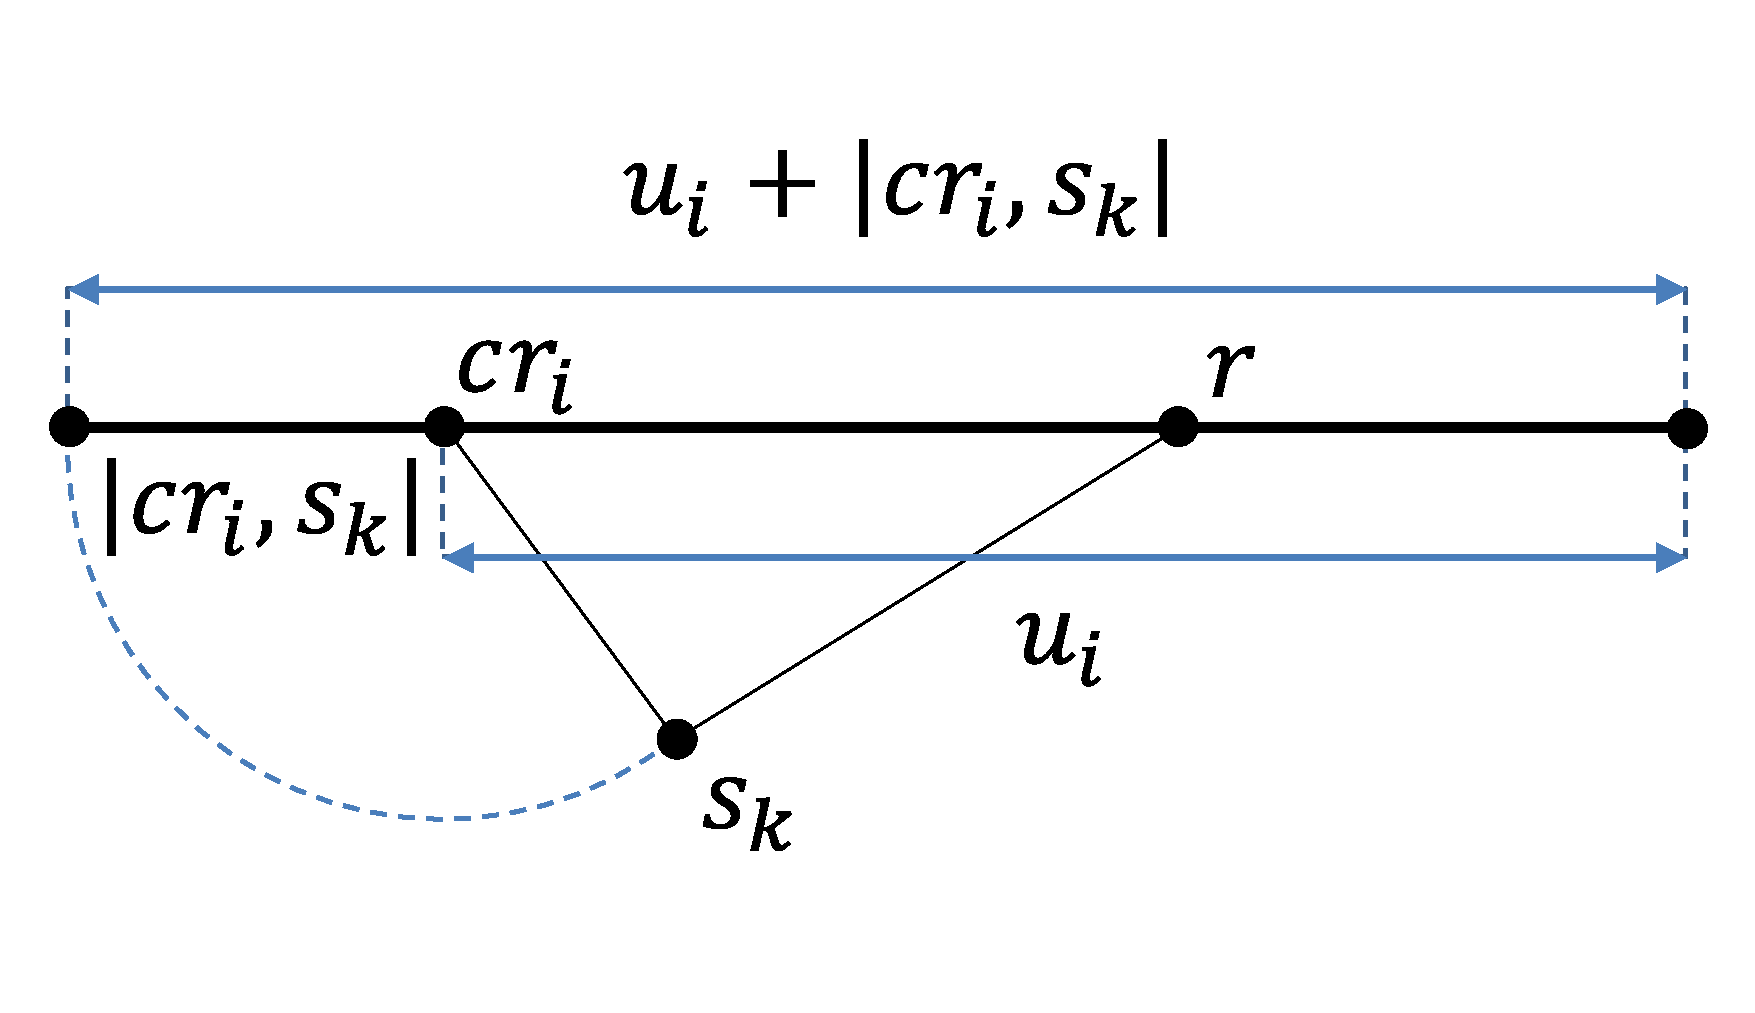
\includegraphics[width=1.6in]{figs/knnjbound1}
% 		\label{fig:knnjbound1}}
% 	\subfigure[\small Bound centers at $cr_i$]{
% 		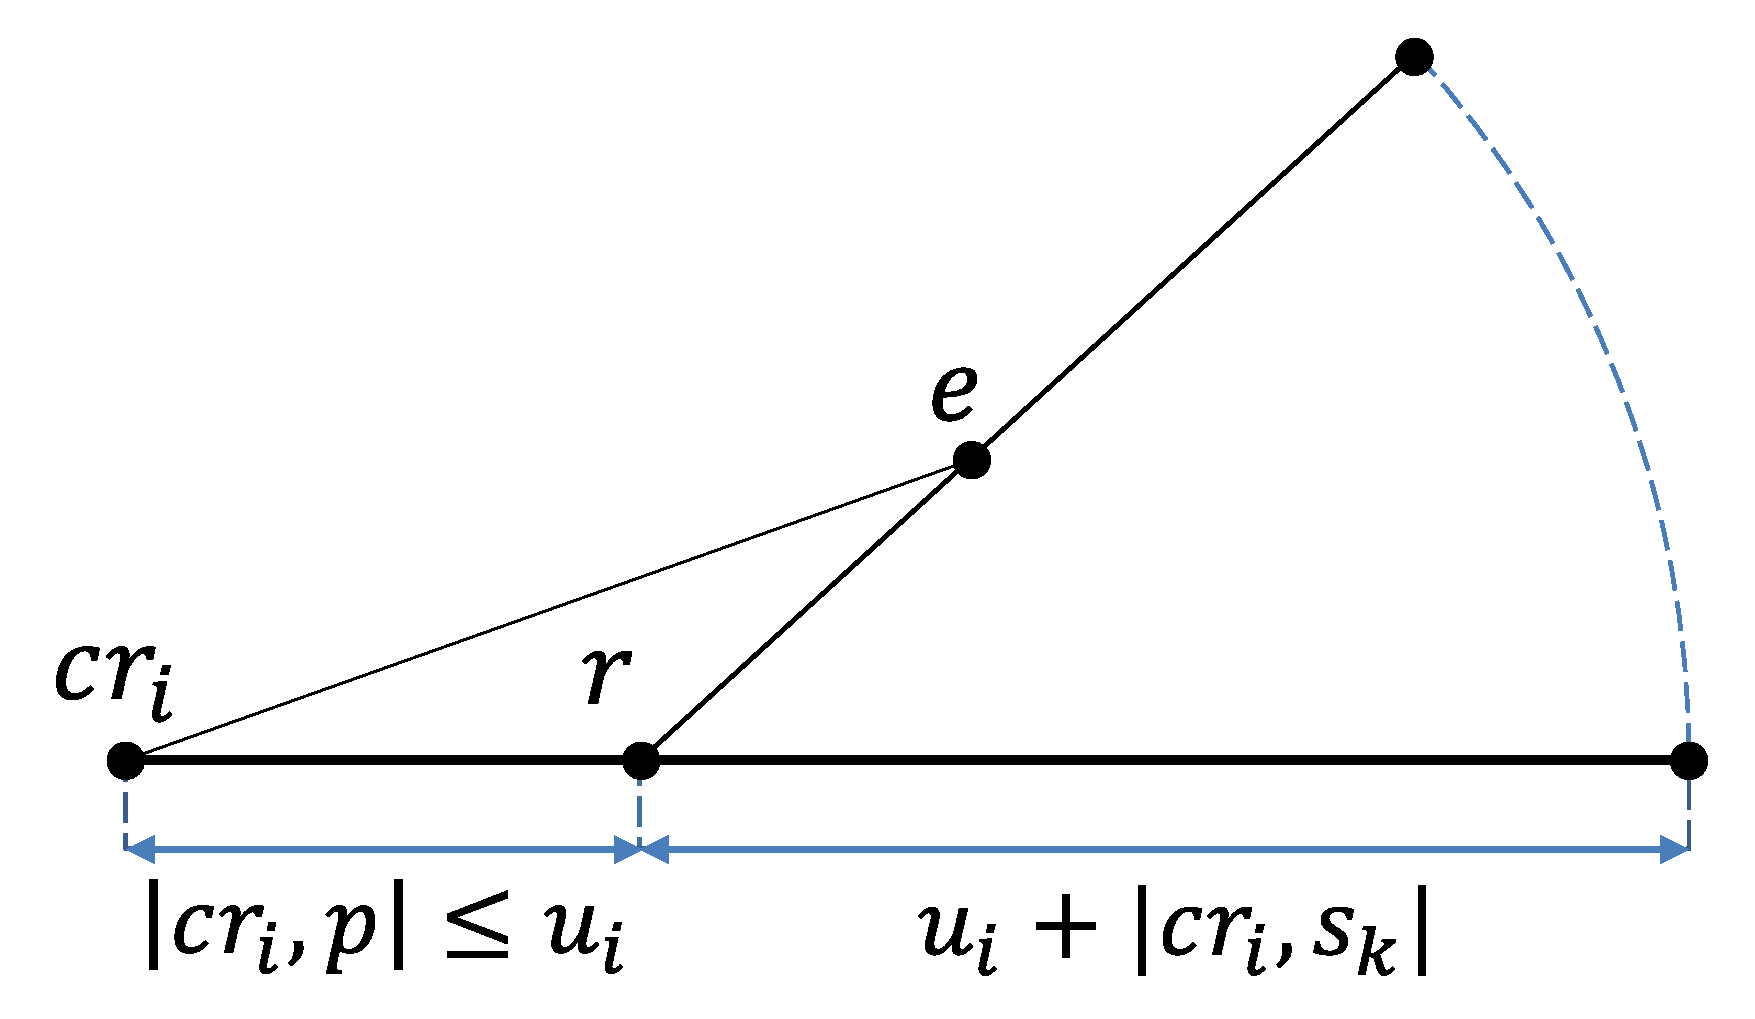
\includegraphics[width=1.6in]{figs/knnjbound2}
% 		\label{fig:knnjbound2}}
%       \caption{Distance bound for RKJ-Spark.}\vspace{-4mm}
% 	\label{fig:knnjbound}
% \end{figure}

The key idea in RKJ-Spark is to derive a distance bound $\gamma_i$ for
each $R_i$, such that we can use $\gamma_i$, $R_i$, and $T$ to find a
subset $S_i\in S$ so that for any $r\in R_i$, $\knn(r, S)=\knn(r,
S_i)$. This partitioning strategy ensures that $R \Join_{\knn} S =
(R_1 \Join_{\knn} S_1) \bigcup (R_2 \Join_{\knn} S_2)\bigcup \cdots
\bigcup (R_n \Join_{\knn} S_n)$, and allows the parallel execution of
only $n$ local $k$NN joins (every $(R_i, S_i)$ pair for $i\in[1, n]$)).


We use $cr_i$ to denote the centroid of $\mbr(R_i)$. First, in
parallel for each $R_i$, \name finds the distance $u_i$ from the
furthest point in $R_i$ to $cr_i$, i.e., $u_i=\max_{r\in R_i}|r,
cr_i|$. \name sends these $u_i$ values and centroids back to the
master node.

Next, the driver program on the master node finds $\knn(cr_i, S')$
using the R-tree $T$ for $i\in[1, n]$. Without loss of generality,
suppose $\knn(cr_i, S')=\{s_1, \ldots, s_k\}$ (in ascending order of
their distances to $cr_i$). Finally, \name simply sets:
\begin{equation}
\label{eq:rkjbound}
 \gamma_i= 2u_i +|cr_i, s_k| \textrm{ for partition $R_i$},
\end{equation}
and finds $S_i=\{s|s \in S, |cr_i, s|\leq \gamma_i\}$ using a circle
range query centered at $cr_i$ with radius $\gamma_i$ over $S$. This
guarantees the desired property as described above, due to:
\vspace{-3mm}
\begin{theorem}
\label{thm:rtknnj}
For any partition $R_i$ where $i \in[1, n]$, we have:
\[\forall r \in R_i, \knn(r, S) \subset \{s|s \in S, |cr_i, s| \leq
\gamma_i\},  \textrm{ for }\gamma_i \textrm{ defined in }\eqref{eq:rkjbound}.\]
\end{theorem}
The proof is shown in Appendix \ref{sec:proof1}.  This leads to the
design of RKJ-Spark. Specifically, for every $s \in S$, RKJ-Spark
includes a copy of $s$ in $S_i$ if $|cr_i, s| \leq \gamma_i$. Theorem
\ref{thm:rtknnj} guarantees that for any $r\in R_i$, $\knn(r,
S)=\knn(r, S_i)$.

Thus, \name invokes a \texttt{zipPartitions} operation for each
$i\in[1, n]$ to place $R_i$ and $S_i$ together into one RDD
partition. In paralle, on each such RDD partition, \name builds a
R-tree over $S_i$ and executes a local $k$NN join using $R_i$ over
this tree. The union of these $n$ outputs is the final answer for
$R\Join_{\knn}S$.

%Though sharing basic ideas with Voronoi $k$NN join, R-Tree $k$NN join
%requires less computations when partitioning input tables and
%calculating distance bounds. Besides, it avoids geometric grouping
%which is used to keep load balance and control the number of local
%$k$NN join tasks. Generally speaking, compared with Voronoi $k$NN join,
%R-Tree $k$NN join is much easier to implement and achieves comparable
%performance as well (see experiment results in Section \ref{sec:exp}).


%%% Local Variables:
%%% mode: latex
%%% TeX-master: "paper"
%%% End:

\section{Query Optimization}
\label{sec:opt}
\name tunes system configurations and optimize complex spatial queries
automatically to make the best use of existing indexes and
statistics. We employed a cost model for determining a proper number
of partitions in different query plans. We also added {\em new logical
  optimization rules} and {\em cost-based optimizations} to the
catalyst optimizer and the physical planner in Spark SQL.

Number of partitions plays an important role in performance tuning in
Spark.  A good choice on the number of partitions not only guarantees
no crashes caused by memory overflow, but also improves throughput and
reduces latency. Given the memory available on a worker node in the
cluster and the input data size, \name partitions the data such that
each partition has roughly equal number of records and they fit into
the memory size of a worker node. This ensures load balancing in the
cluster.

% In \name, we build a cost model to estimate the partition size under a
% schema. It handles two cases: tables with fixed length records and
% tables with varible length record. The first case is simple to
% handle. The cost model estimates the size of a partition based on
% record size $z$, number of records ($m$) that goes into a partition
% (once given a partition strategy), and an estimation of the index size
% (calculated based on the values of $z$ and $m$, and the index type).
% The variable length record case is much harder, since it is difficult
% to estimate the size of a partition even if we know how many recrods
% are going into a partition (e.g., say we have used an equi-depth
% partition strategy to partition the table using a nubmer of quantile
% values so that each partition has roughly same number of records). It
% is also difficult to estimate the size of an index in this
% case. Currently, \name resolves this challenge using a sampling based
% approach, but there is no formal guarantees that the samples will
% always lead to good partitions in the end over the original data.

% Using the cost model and a specified partition strategy, \name then
% computes a good value for the number of partitions such that: 1)
% partitions are balanced in size; 2) size of each partition fits the
% memory size of a worker node; and 3) the total number of partitions is
% proportional to the number of workers in the cluster.  Note that the
% size of a partition should be close but not greater than a threshold,
% which indicates how much heap memory Spark can reserve for query
% processing. In Spark, on each slave node, a fraction of memory is
% reserved for RDD caching, which is specified as a system configuration
% \texttt{spark.storage.memoryFraction} (we denote this value as
% $\alpha$). In our cost model, the remaining memory will be evenly
% split to each processing core. Suppose the number of cores is $c$ and
% total memory reserved for Spark on each slave node is $M$. The
% partition size threshold $\beta$ is then calculated as:
% $\beta =\lambda ((1-\alpha) M / c) $, where $\lambda$ is a system
% parameter, whose default value is 0.8, to take memory consumption of
% run-time data structures into consideration.  With the cost model,
% \name can determine the number of records for a single partition, and
% the numbers of partitions for different data sets.

To better utilize the index support in \name, we add new rules in the
catalyst optimizer to select those predicates which can be optimized
by indexes. First, we transform the original select condition to {\em
  Disjunctive Normal Form} (DNF), e.g.
$(A \wedge B) \vee C \vee (D \wedge E \wedge F)$.  Then, we get rid of
all predicates in the DNF clause which cannot be optimized by indexes
to form a new select condition $\theta$. \name will filter the input
relation with $\theta$ first using index-based operators, and then
apply the original select condition to get the final answer.

% get the final results. We term this procedure as indexed table scan
% optimization.

\begin{figure}[t!]
	\centering
	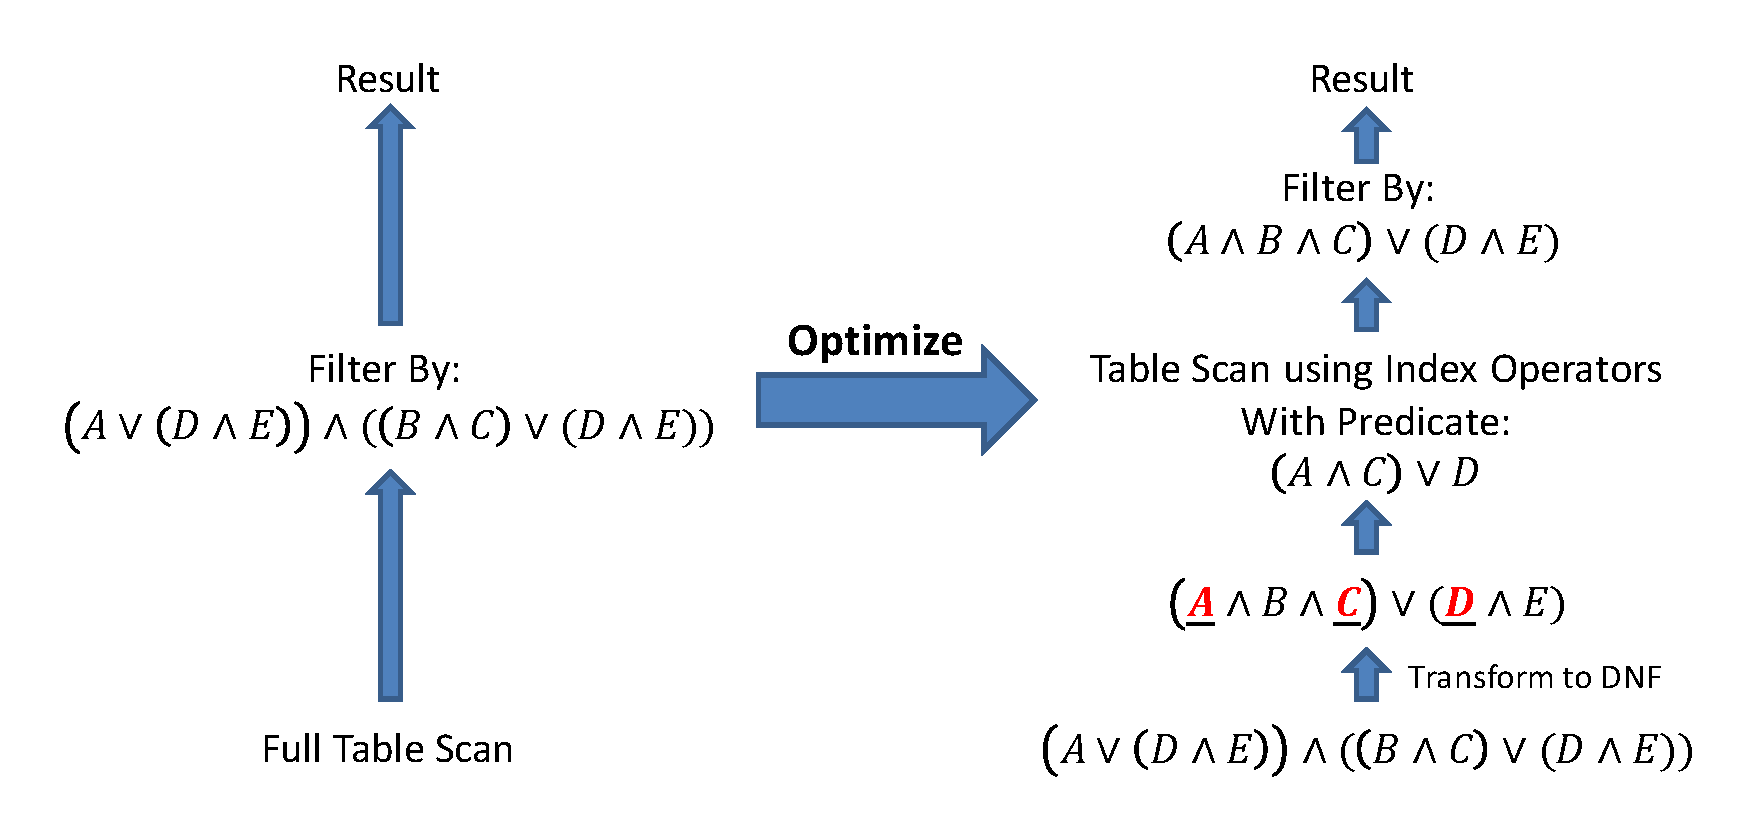
\includegraphics[width=3.4in]{figs/optimize}
	\vspace{-8mm}
	\caption{Index scan optimization in \name.}
	\label{fig:optimize}
	\vspace{-4mm}
\end{figure}

Figure \ref{fig:optimize} shows an example of the index scan
optimization. The select condition on the table is
$(A \vee (D \wedge E)) \wedge ((B \wedge C) \vee (D \wedge E))$.
Assuming that $A$, $C$ and $D$ can be optimized by utilizing existing
indexes. Without index optimization, the engine (e.g., Spark SQL)
simply does a full scan on the table and filters each record by the
input select condition. By applying index optimization, \name works
out the DNF of select condition, which is
$(A \wedge B \wedge C) \vee (D \wedge E)$, and invokes a table scan
using index operators under a new condition $(A \wedge C) \vee D$.
Then, we filter the resulting relation with original condition once
more to get the final results.

\name also explores various {\em geometric properties} to merge
spatial predicates in order to reduce the number of physical
operations. Generally, we merge predicates on single dimension into
segments or bounding boxes, which can be processed together without
involving expensive intersections or unions on intermediate
results. For example, \texttt{x > 3 AND x < 5 AND y > 1 AND y < 6} can
be merged into a range query on \texttt{(POINT(3, 1), POINT(5, 6))},
which is natively supported in \name as a single range query. \name
also merges query segments or bounding boxes prior to execution, so
that it greatly reduces the number of operations. For instance, two
conjunctive range queries on \texttt{(POINT(3, 1), POINT(5, 6))} and
\texttt{(POINT(4, 0), POINT(9, 3))} can be merged into a single range
query on \texttt{(POINT(4, 1), POINT(5, 3))}.

Index optimization improves performance greatly when the predicates
are selective.  However, it may cause more overheads than savings when
query selectivity is low or the size of input table is small. Thus,
\name also uses a new cost based optimization (CBO), which takes
existing indexes and statistics into consideration, to choose the most
efficient physical plans on the fly. Specifically, \name will estimate
the query selectivity using indexes and simple statistics on
tables. % issue a fast partial query to existing indexes so as to get an
% upper bound of condition selectivity. Besides, it will check the
% size of input relation.
If query selectivity is low or the size of input relation is small,
\name will scan the table without utilizing indexes.

CBO is also used for joins in \name. When one of the tables in the
join is small (much smaller compared to the other table), \name's
optimizer will switch to a {\em broadcast join} algorithm by skipping
the data partition phase on the small table, and broadcast the small
table to every partition of the large table to do local joins. For
example, if $R$ is small and $S$ is big, \name will do local joins
over $(R, S_1), \ldots, (R, S_m)$. This applies to both distance and
$k$NN joins.


For $k$NN joins in particular, CBO is used to do fine-tuning for the
RKJ-Spark algorithm. We can increase the sampling rate used to
generate $S'$ and/or partition table $R$ with finer granularity, to
get a tighter bound for $\gamma_i$. \name's optimizer adjusts the
sampling rate of $S'$ according to the memory size on the master node
(and the max possible query value $k_{\max}$ so that $|S'|>k_{max}$;
typically $k$ is small for $k$NN queries). \name's optimizer can also
invoke another STR partition {\em within each local partition} to get
partition boundaries {\em locally on each worker} with finer
granularity without changing the global partition and physical data
distribution. This allows RKJ-Spark to compute tighter bound for
$\gamma_i$ using the refined partition boundaries, thus reduce the
size of $S_i$'s.


Lastly, \name uses a SQL context that is thread-safe (using
thread-local instances for conflicts) to support the execution of
multiple queries concurrently, hence, multiple users can issue queries
concurrently to the same \name instance.


% In Spark 1.3.0 (which is the base system of SparkSpatial), SQL
% context cannot support multiple queries concurrently, as numbers
% of components (e.g. SQL parser, catalyst optimizer) in Spark SQL
% are not thread-safe. To address this problem, SparkSpatial sepa-
% rates such conflict components into thread-local instances. As a re-
% sult, multiple users can now issue queries concurrently to the same
% SparkSpatial instance.

% \SparkSpatial is able to optimize complex queries automatically to
% make the best use of existing table indexes and statistics. We
% extend the catalyst optimizer and the physical planner of Spark SQL
% with new rules to dig out more possibilities for optimizations
% brought by table indexing.

% With the help of table indexes, plenty of operations can achieve
% orders of magnitude better performance than that in the non-index
% cases. \SparkSpatial picks the predicates that can be optimized by
% leveraging table indexes from the original query condition and
% processes them first to shrink the data size as soon as
% possible. Specifically, we first transform the original query
% condition to \emph{Disjunctive Normal Form} (DNF) and select the
% predicates that can be accelerated by existing indexes. Then, we
% only keep the selected predicates in DNF as a new query condition
% and use index-version algorithms (implemented in
% \texttt{IndexRelationScan}) to filter the original data set. To get
% the final result, \SparkSpatial processes the original condition
% once again on the filtered data. This time, it will be much more
% efficient since data size shrinks dramatically in the last step.

% For instance, $A, B, C, D, E$ are predicates from the original query
% condition and DNF of this condition is $(A \wedge B \wedge C) \vee
% (D \wedge E)$. Assuming that $A$, $C$ and $D$ can be optimized by
% utilizing existing indexes, we process $(A \wedge C) \vee D$ in
% \texttt{IndexRelationScan} first to shrink the data size. Next, $(A
% \wedge B \wedge C) \vee (D \wedge E)$ is applied on the shrunk data
% so as to get the final results.

% In addition to optimize query conditions with existing indexes,
% \SparkSpatial also merges predicates to reduce the number of
% physical operations. For example, \texttt{x > 3 AND x < 5 AND y > 1
% AND y < 6} can be merged as a single spatial predicate \texttt{(x,
% y) in RANGE(POINT(3, 1), POINT(5, 6))}, which can be optimized as a
% box range query when there is an R-Tree index built on attribute
% \texttt{x} and \texttt{y}.

% In Spark 1.3.0 (base system of \SparkSpatial), numbers of components
% (e.g. SQL Parser, catalyst optimizer) in Spark SQL are not thread
% safe, which makes Spark SQL unable to support concurrent query
% perfectly. We address this issue by separating these conflict
% components into thread-local instances. Thus, \SparkSpatial can
% support concurrent queries issued by multiple users in the same
% \SparkSpatial instance.


%%% Local Variables:
%%% mode: latex
%%% TeX-master: "paper"
%%% End:

\section{Experiment}
\label{sec:exp}
% We have conducted a comprehensive experimental evaluation on the
% performance of \name and also compared \name with other closely
% related systems.

\subsection{Experiment Setup}
\label{sec:setupexp}
All experiments are conducted on a cluster consisting of 10 nodes with
two configurations: (1) 8 machines with a 6-core Intel Xeon E5-2603 v3
1.60GHz processor and 20GB RAM; (2) 2 machines with a 6-core Intel
Xeon E5-2620 2.00GHz processor and 56GB RAM. Each node is connected to
a Gigabit Ethernet switch and runs Ubuntu 14.04.2 LTS with Hadoop
2.4.1 and Spark 1.3.0. We select one machine of type (2) as the master
node and the rest are slave nodes. The Spark cluster is deployed in
standalone mode and configured to use up to 15GB memory on each slave
node. We used the following real and synthetic datasets: \vspace{-1mm}
\begin{pkl}
\item OSM: OSM is a real dataset extracted from the OpenStreetMap
  project \cite{osm}.  We took uniform random samples of various size
  (1 million to 1 billion records) from the complete OSM data set and
  used them in our experiments. Each record contains a rid,
  2-dimensional coordinate, time stamp and description.
  \dong{new experiments rely on only rid and two coordinates.}
\item GDELT: GDELT stands for Global Data on Events, Language and Tone
  \cite{gdelt}, which is an open database of human society, containing
  75 million records in total. In our experiment, each record takes 7
  attributes: a timestamp, and three 2-dimensional coordinates which
  represent the locations for the start, the terminal, and the action
  of an event.
\item RC: We also generated synthetic datasets of various sizes (1
  million to 1 billion records) and dimensions (2 - 6 dimensions)
  using a {\em random cluster} generator with Gaussian
  distributions. Each record in $d$-dimension contains $d+1$
  attributes: namely, a record ID and its spatial coordinates.
\end{pkl}\vspace{-2mm}

For single-relation operations (i.e. range and $k$NN queries), we
evaluate the performance with two metrics: {\em throughput and
  latency}. In particular, for both \name and Spark SQL, we run a
Spark instance with thread pool size = 10 in the driver program, and
issue 500 queries to the system to calculate the throughput. For other
systems that we reviewed in Section \ref{sec:background}, since they
do not use a multi-threading model, we submit 20 queries at the same
time, and run them as 20 different processes to ensure full
utilization of the cluster resource. The throughput is calculated by
dividing the total number of queries over the running time. Note that
this follows the same way these systems had used to measure their
throughput \cite{spatialhadoop}.  For all systems, we used 100
randomly generated queries to measure the average query latency.

For join operations, we focus on the average running time of a join
query over 10 randomly generated join queries for all systems.

In all experiments, HDFS block size is 64MB. By default, $k=10$ for a
$k$NN or a $k$NN join query. A range query is characterized by its
{\em query area, as a percentage over the entire area} that data
locate at. The default for range queries is $0.01\%$. The default
distance threshold $\tau$ for a distance join is set to $5$ (each
dimension is normalized into a domain from $0$ to
$1000$).% the area for a
% circle with radius $\tau=x$ retrieves roughly $y$ number of points
% {\em on average} from the second table.  $0.00005\%$ of the entire
% area.
The default partition size is is $500\times 10^3$ (500k) records per
partition. The default data set size for single-relation operations is
500 million records on OSM and 700 million on synthetic data sets, and
3 million records in each input table for a join. The default
dimensionality is 2.

%\feifei{Specify $x$ and $y$ above.}


% , and $3\times10^4$
% records.% Expected partition size for table indexing is $5\times10^5$ records
% by default, while that for joins is $3\times10^4$ records.

% \dong{We should not set default values on sample rate and expected
%   partition size here since we claim that \name will automatically
%   tune these configurations.}


\subsection{Cost of Indexing}
\label{sec:indexexp}
We first investigate the cost of indexing in \name and other
cluster-based spatial analytics systems, including SpatialSpark
\cite{spatialspark}, SpatialHadoop \cite{spatialhadoop}, and Hadoop
GIS \cite{hadoopgis}. Figure \ref{fig:index_datasize} presents the
index construction time in different systems on OSM data, when OSM
varies from 30 million to 1 billion records. As shown in the figure,
\name has the best performance among all systems and scales linearly
to the size of the data as well. For example, \name builds its index
(which uses R-tree for both local indexes and the global index) over
1 billion records, 60GB in file size, in around 25 minutes, which is
2.5x faster than SpatialHadoop, 3x faster than SpatialSpark, and 12x
faster than Hadoop GIS. Note that GeoSpark is faster than all of
other systems because it only uses Spark's default partitioner
without spatial locality and build local indexes on each partition,
thus does not involve data repartitioning and global indexing. Compared
to Hadoop based systems, \name indexes RDDs, while Hadoop-based systems
index HDFS file blocks. Even though SpatialSpark also uses Spark, but
it {\em does not} index RDDs natively. Instead, it indexes files in HDFS
as well.


%We do not include the result of GeoSpark because
%it only supports local indexing and does not provide a spatial RDD
%partitioner according to its latest open-sourced version (0.2.0).
%Thus, we are unable to compare it with other systems which has
%full support on data partition, local indexing and global indexing.


\begin{figure}[t]
	\centering
	\subfigure[Effect of data size (OSM).]{
		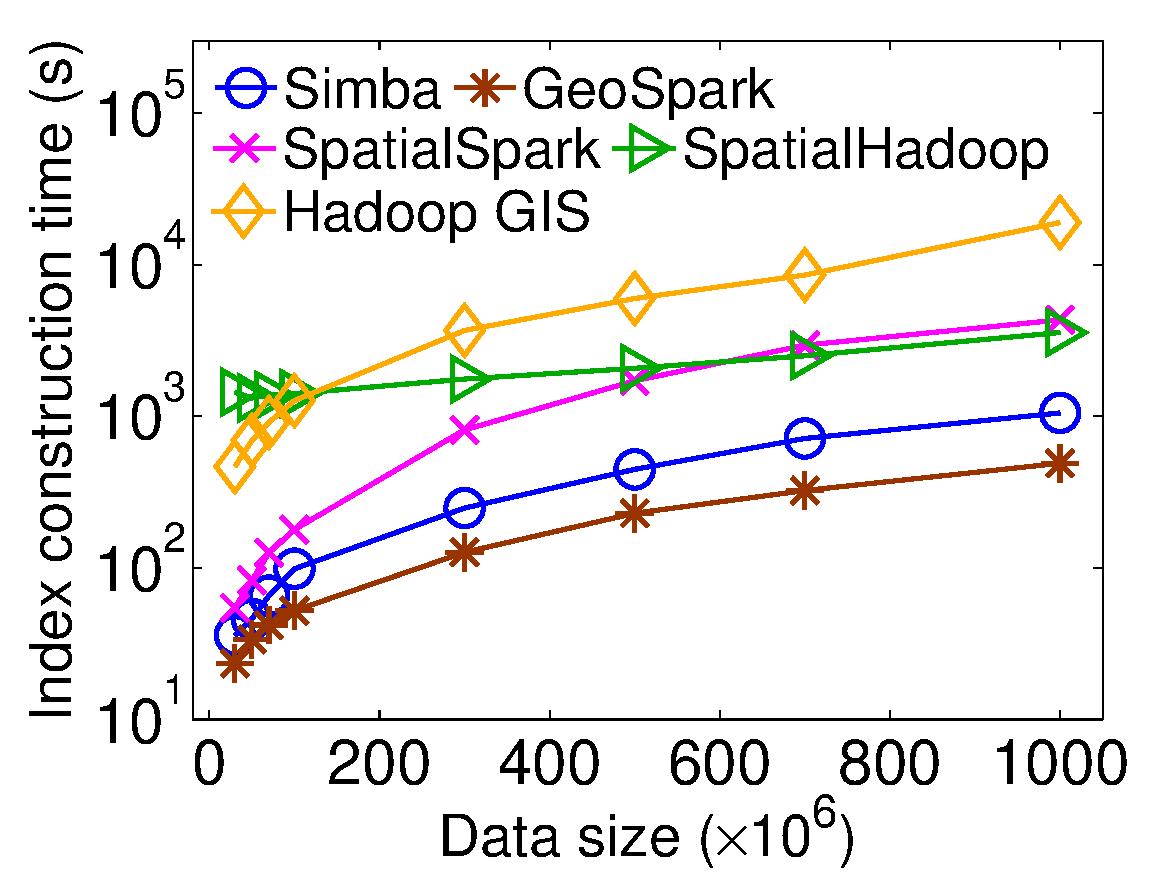
\includegraphics[width=1.55in]{figs/exp/index_time}
		\label{fig:index_datasize}}%\vspace{3mm}
	% \subfigure[Effect of partition size.]{
	% 	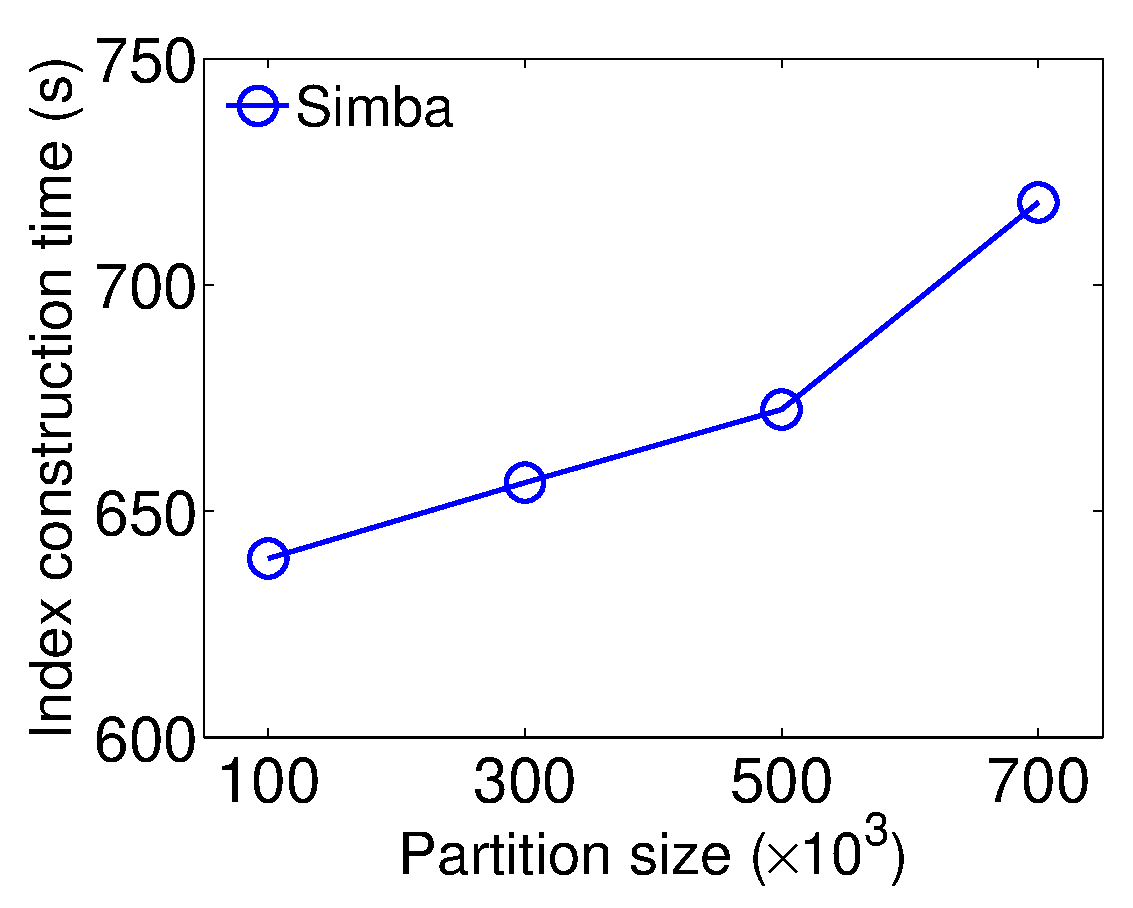
\includegraphics[width=1.55in]{figs/exp/osm_index_partsize_time}
	% 	\label{fig:index_partsize}}
	\subfigure[Effect of dimensionality.]{
		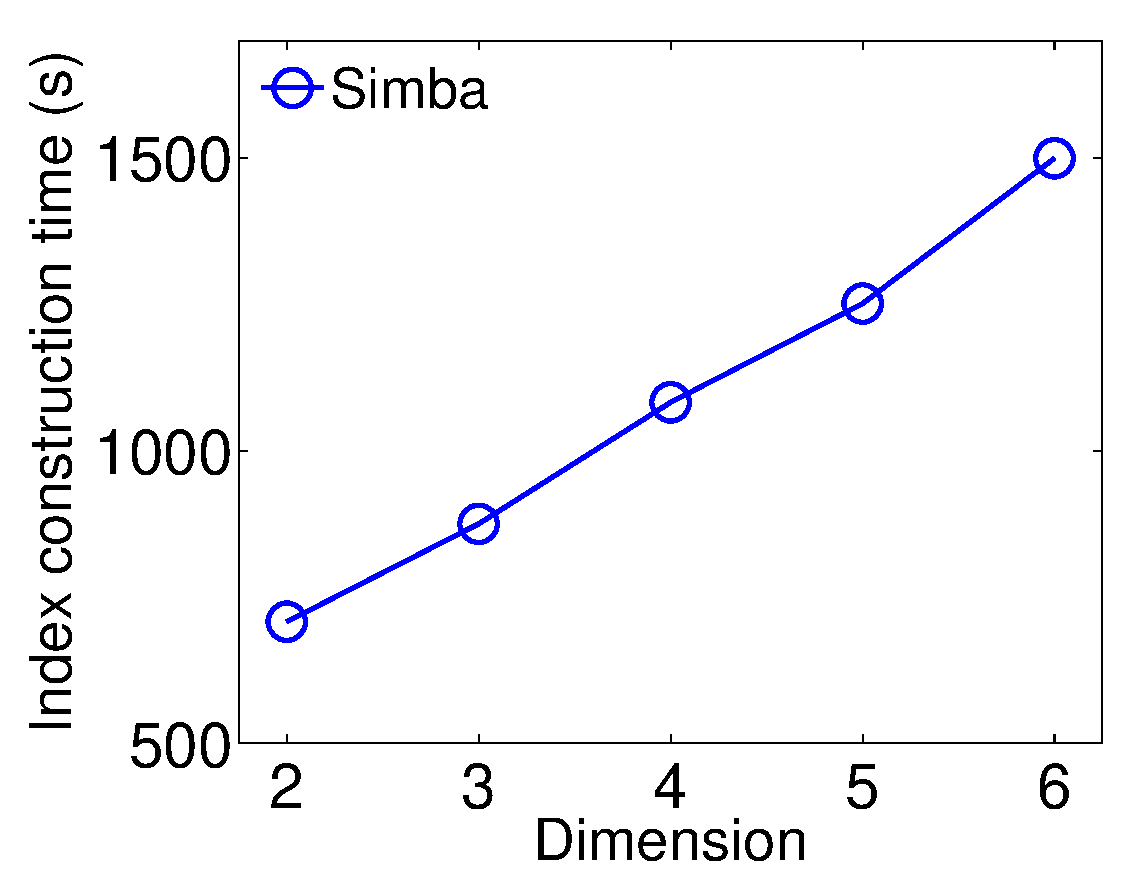
\includegraphics[width=1.55in]{figs/exp/index_dim_time}
		\label{fig:index_dim}}
	\caption{Index construction cost.}\vspace{-4mm}
	\label{fig:indexexp}
\end{figure}

We then investigated \name's index support in higher
dimensions. Figure \ref{fig:index_dim} shows the index construction
time in \name against number of dimensions on the synthetic data
set. The cost increases linearly with the increase in
dimensionality. Note that all {\em other systems can only support up
  to 2 dimensions}.


% Figure \ref{fig:index_partsize} shows that its index construction cost
% grows roughly linearly with respect to (wrt) partition size. This is
% because it is more costly to build local indexes over larger
% partitions (which outweighs the savings resulted from processing less
% number of partitions). % Note that We only show results for
% % \name since expected partition sizes for other systems are fixed to
% % the HDFS block size.


% \begin{figure}[t]
%     \centering
%     \begin{minipage}{1.60in}
%         \centering
%         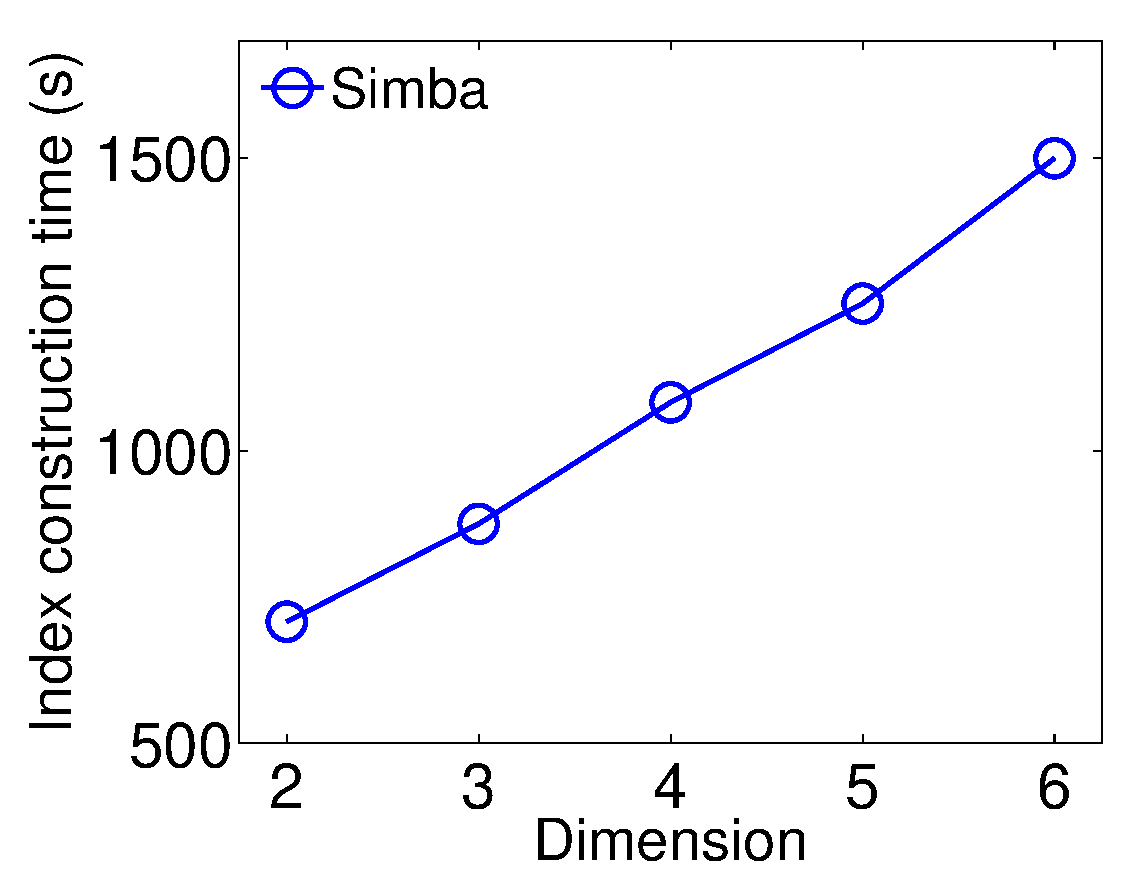
\includegraphics[width=1.50in]{figs/exp/index_dim_time}\vspace{-4mm}
%         \caption{Effect of dimensionality for index construction.}
%     		\label{fig:index_dim}
%     \end{minipage}
%     \hfill
%     \begin{minipage}{1.60in}
%       \centering
%       \vspace{0.5mm}
%       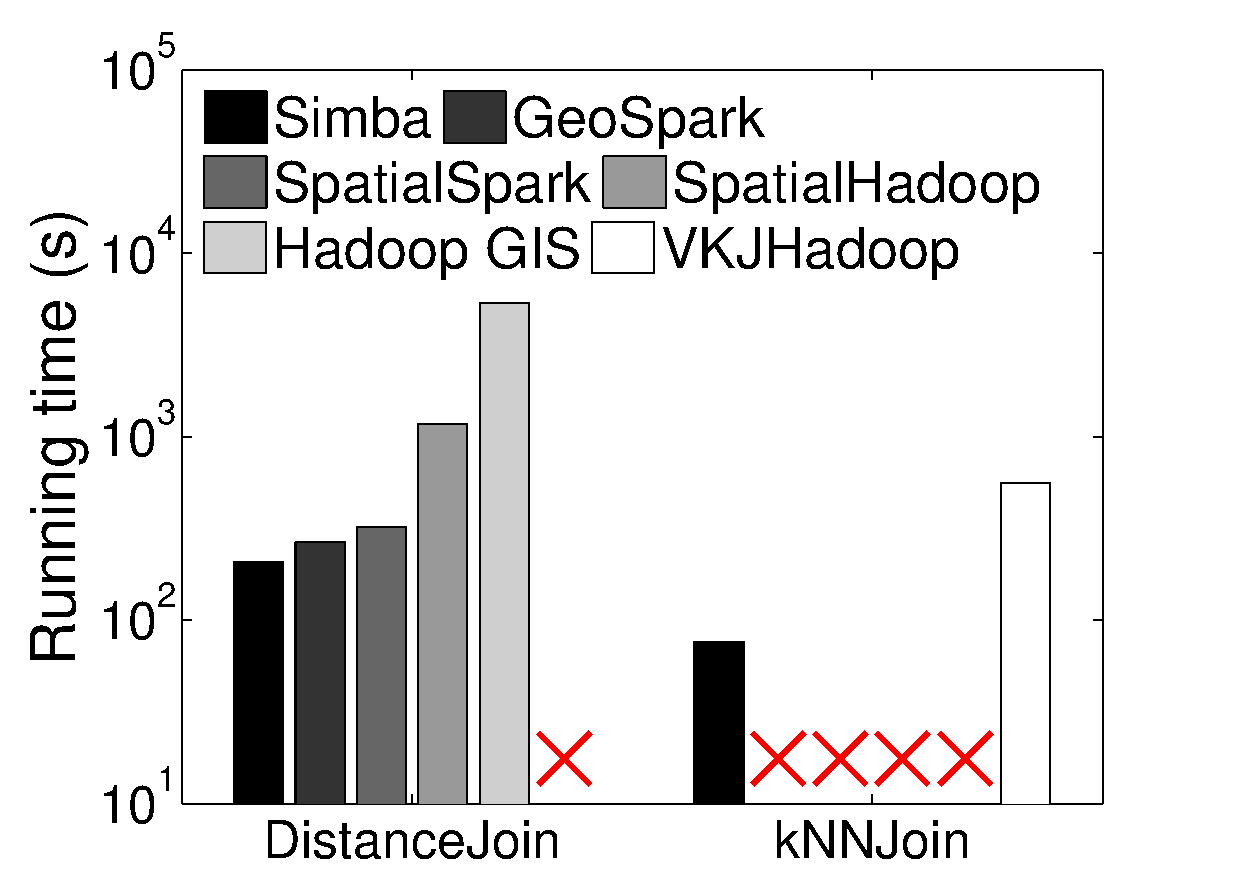
\includegraphics[width = 1.60in]{figs/exp/osm_join_time}\vspace{-2mm}
%       \caption{Join operations on different systems.}
%       \label{fig:system_join}
%     \end{minipage}
%     \vspace{-4mm}
% \end{figure}


\begin{figure}[!t]
	\subfigure[Throughput]{
		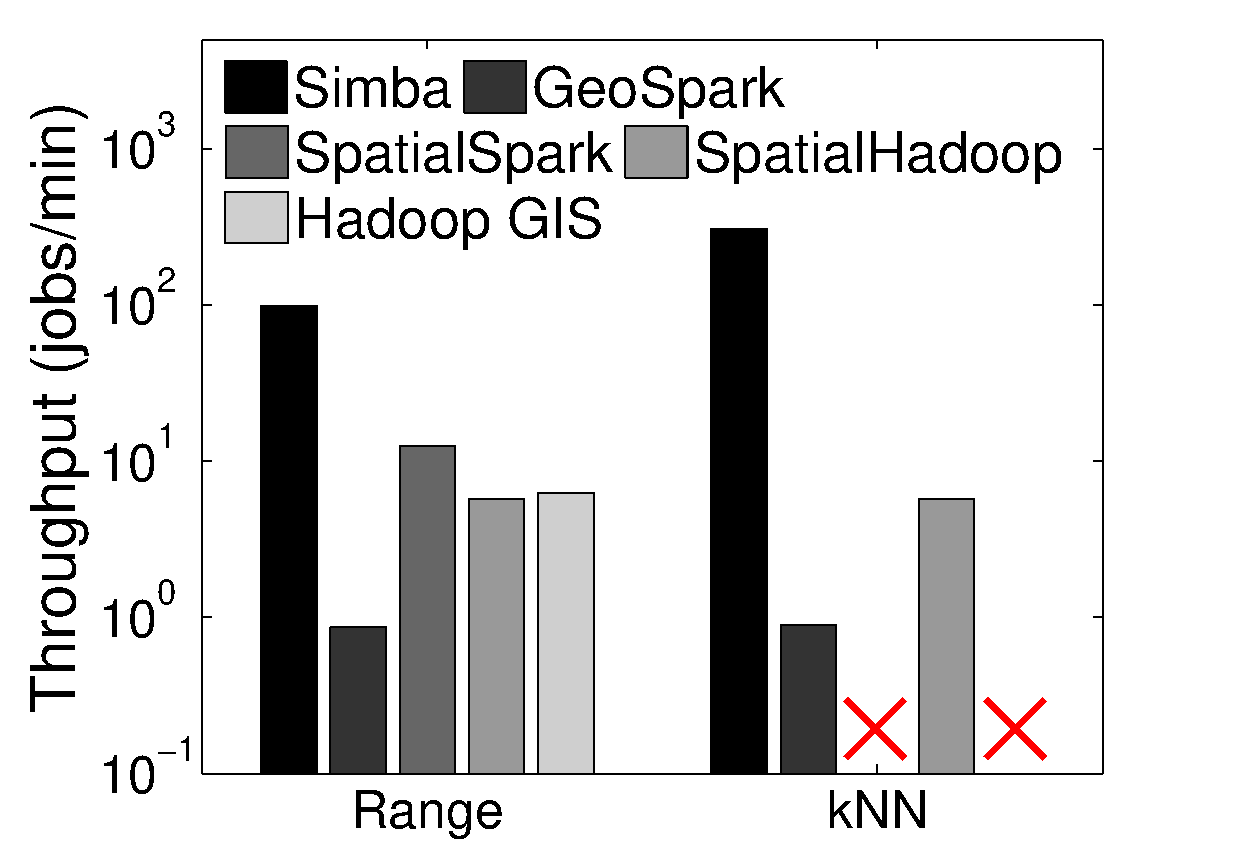
\includegraphics[width=1.55in]{figs/exp/osm_throughput_2}
		\label{fig:system_single_throughput}}
	\subfigure[Latency]{
		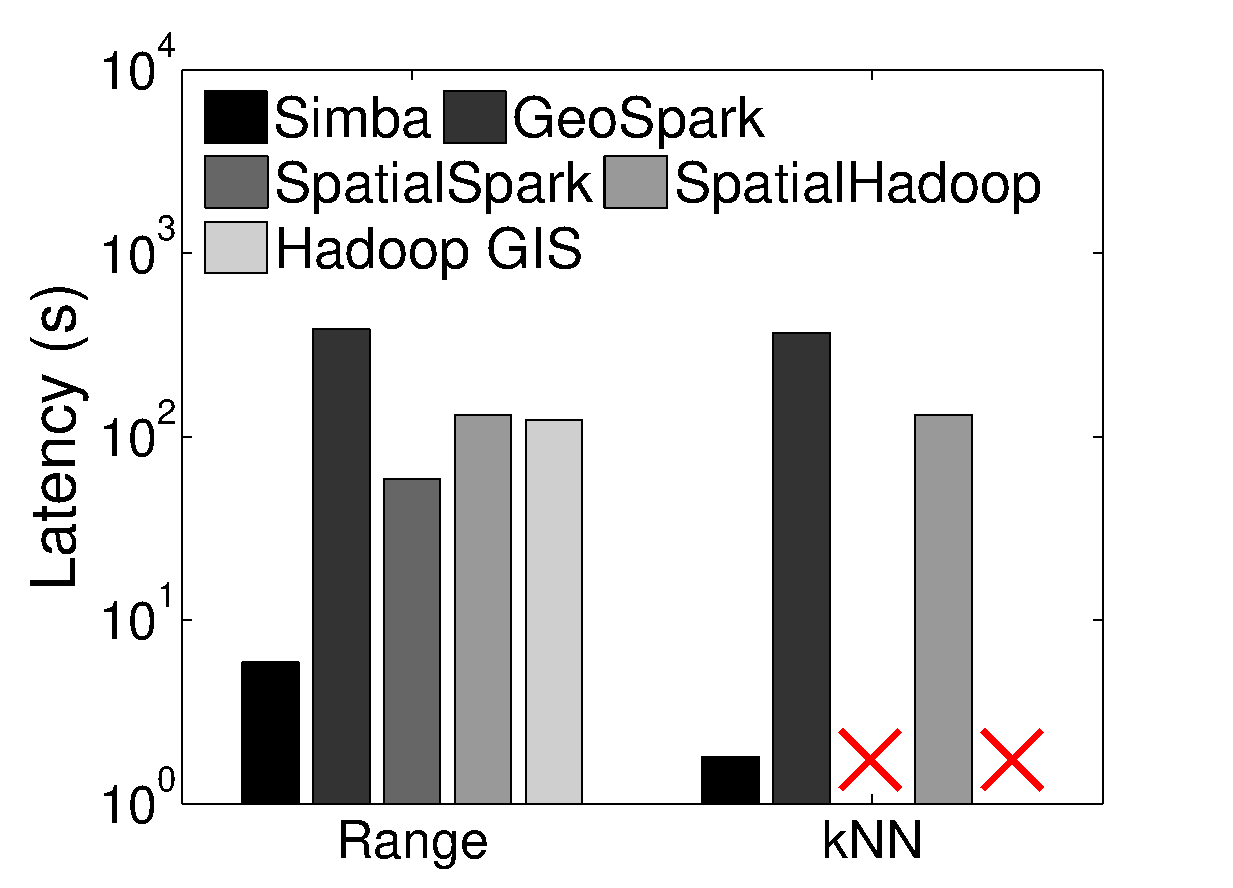
\includegraphics[width=1.55in]{figs/exp/osm_latency_2}
		\label{fig:system_single_latency}}
      \caption{Single-relation operations on different
        systems.}
	\label{fig:system_single}\vspace{-4mm}
\end{figure}

\subsection{Comparison with Existing Spatial Analytics Systems}
\label{sec:comparison}
In this section, we run all spatial operations supported by a system
with the default settings described in Section \ref{sec:setupexp} over
the default OSM dataset (500 million records in 30GB) on \name,
GeoSpark, SpatialSpark, SpatialHadoop, and Hadoop GIS, to compare their
performance.  A red cross mark in the following bar charts indicates
that the corresponding operation is {\em not supported} in a system.


%\vspace{-2mm}
%\begin{figure}[!h]
%	\centering
%	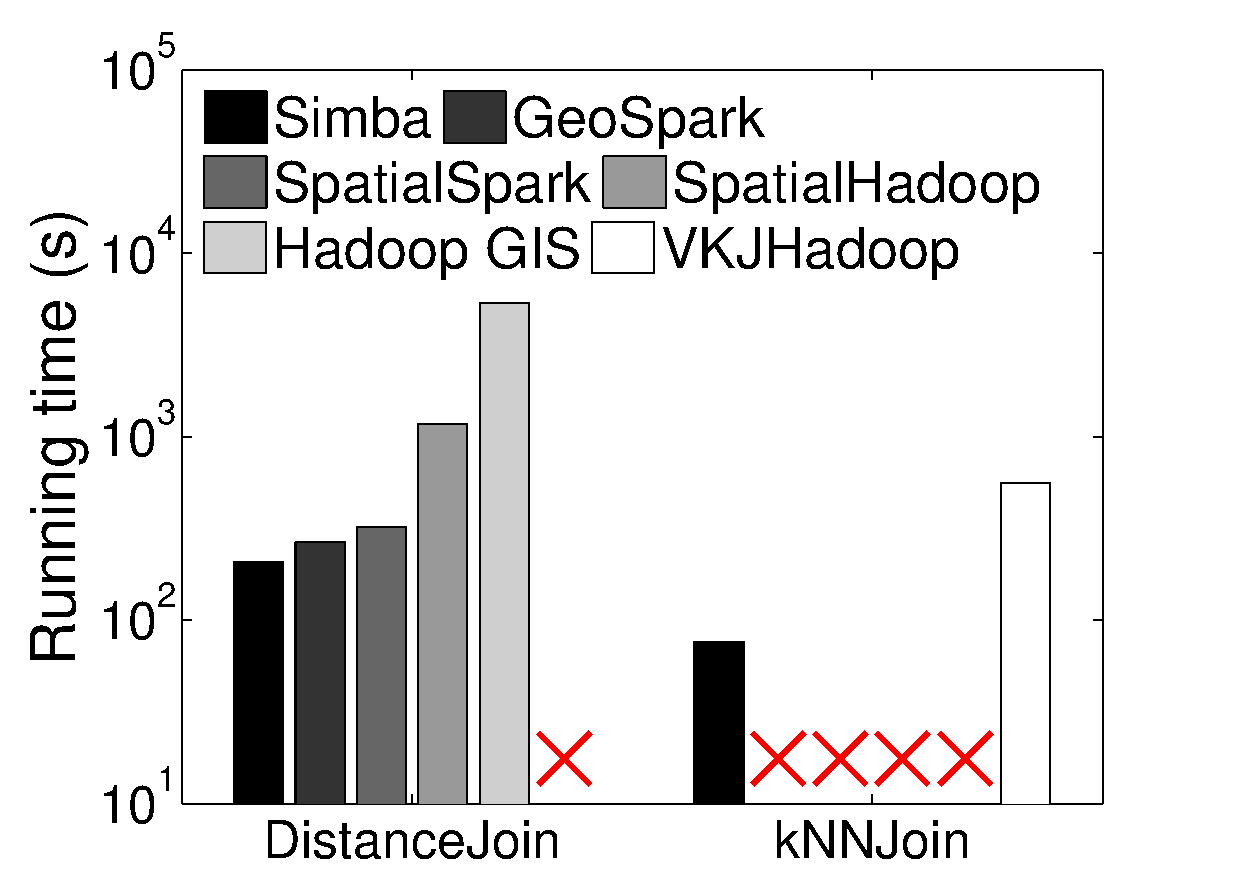
\includegraphics[width = 1.74in]{figs/exp/osm_join_time}\vspace{-4mm}
%	\caption{Join operations on different systems.}
%	\label{fig:system_join}\vspace{-1mm}
%\end{figure}


Figure \ref{fig:system_single} shows the performance of
single-relation operations using both range and $k$NN queries. As
shown in the figure, \name provides the best system throughput and the
best query latency. Specifically, \name achieves 5-50x better
performance (on both throughput and latency) than all existing spatial
analytics systems. Note that the performance of GeoSpark is even worse
than Hadoop based systems because GeoSpark does not leverage global
indexes in query processing, which can help pruning large numbers
of useless partitions (more than 90\%) before scanning them.

% New Range Results of GeoSpark with local indexes.
% Latency: 740.6194
% Througput: 0.6624490742274187

For join operations (using 3 million records in each table), as shown
in Figure \ref{fig:system_join}, \name runs distance join 1.5x faster
than SpatialSpark and 5x faster than Hadoop GIS. Note that distance join
over point objects is not supported in GeoSpark and SpatialHadoop.
GeoSpark supports spatial join between a point RDD and a circle RDD.
Thus, we map each element of $R$ from a point $r$ to a circle object
which centers at $r$ with a radius $\tau$ to a new table $RC(\tau)$.
Immediately, $R \Join_{\tau} S = RC(\tau)\Join_{\textrm{contains}} S$
which is a spatial join. As to SpatialHadoop, it only supports spatial
join over geometric objects, we use $RC(\tau/2)\Join_{\textrm{intersects}} SC(\tau/2)$
to calculate the original distance join.

$k$NN join is not supported by any of these systems. So we compared \name
(using its RKJSpark algorithm) with the Voronoi-based $k$NN join on Hadoop
\cite{vhadoop} (denoted as VKJ-Hadoop), and \name is 7x faster than VKJ-Hadoop.


%       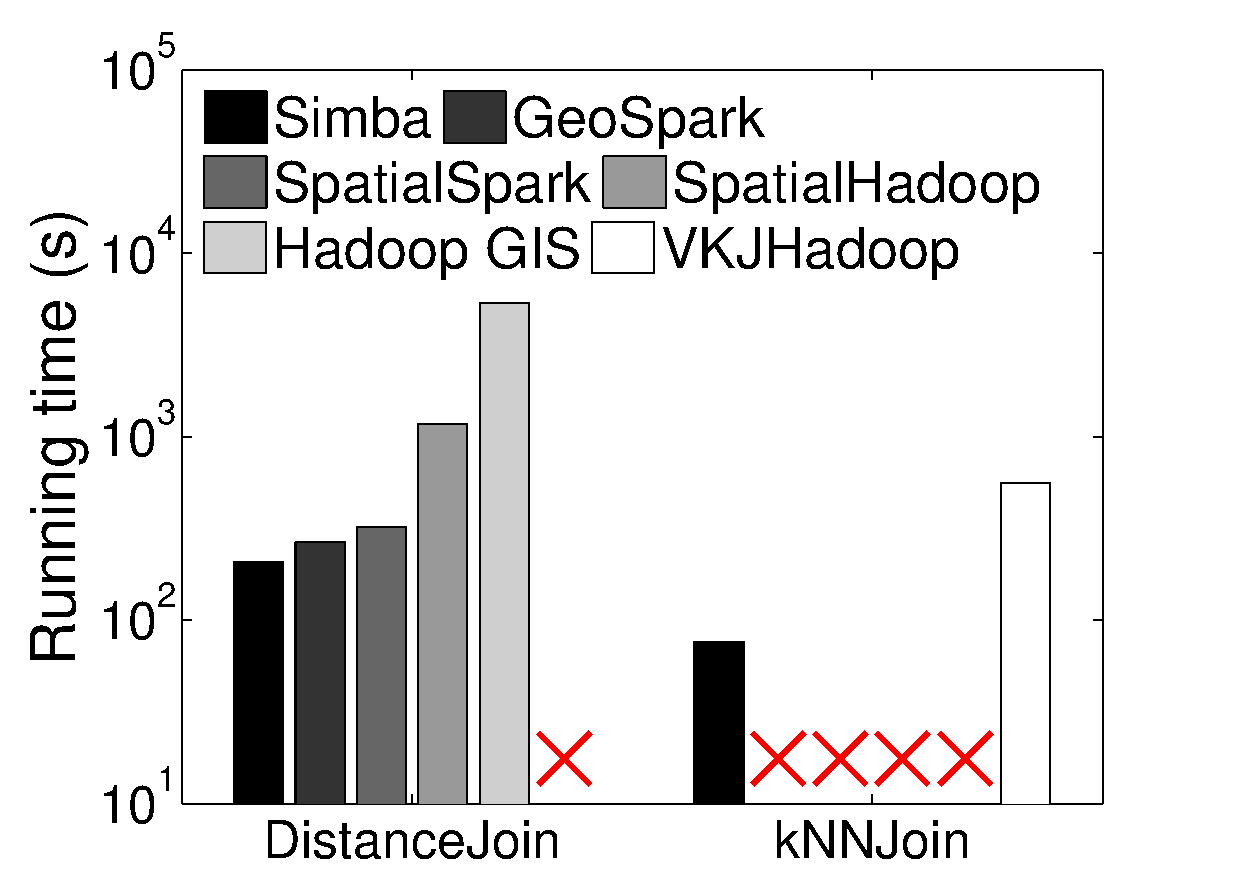
\includegraphics[width = 1.60in]{figs/exp/osm_join_time}\vspace{-2mm}
%       \caption{Join operations on different systems.}
%       \label{fig:system_join}

\begin{wrapfigure}{l}{0.15\textwidth}
 \centering
 \vspace*{-0.2cm}
  \hspace*{-0.3cm}
  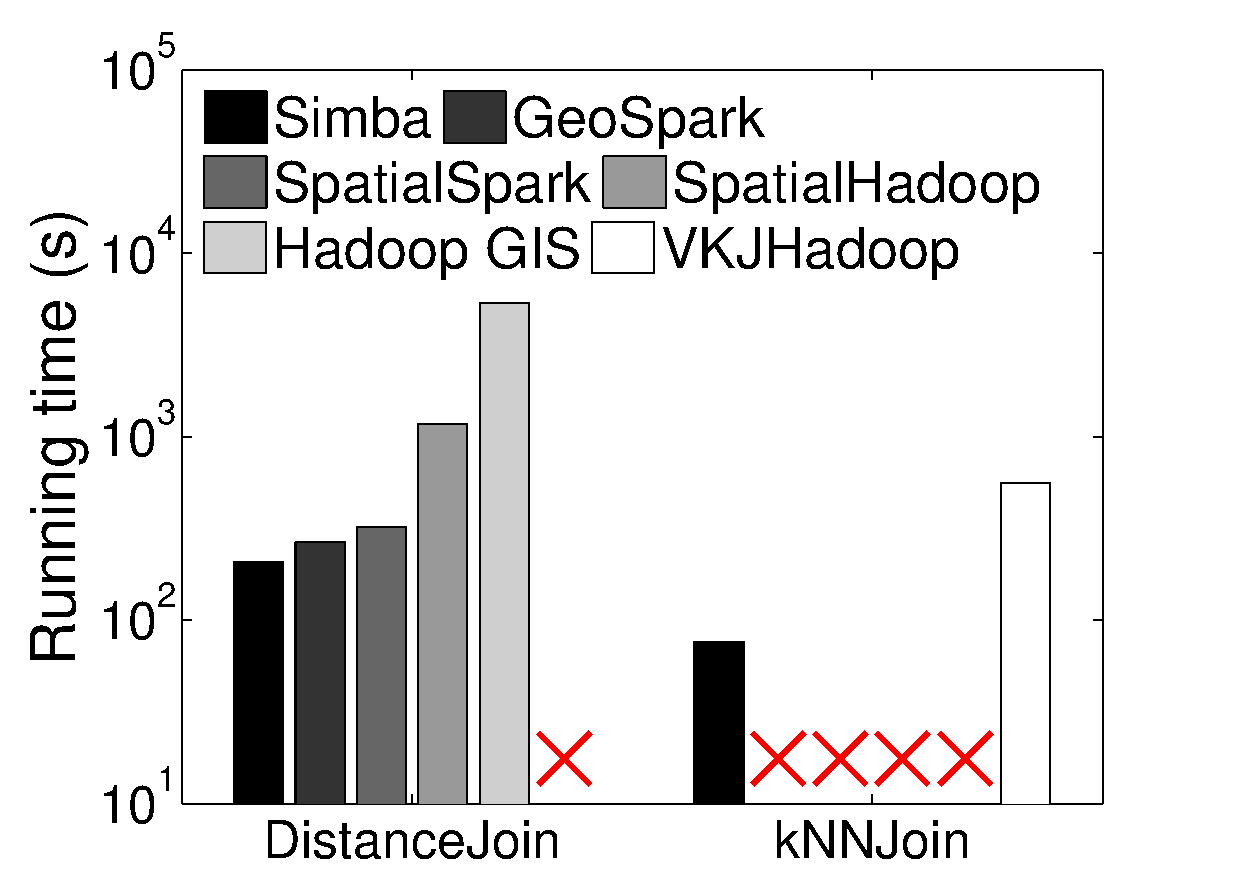
\includegraphics[width=1.5in]{figs/exp/osm_join_time}
  \vspace*{-0.80cm}
  \caption{\label{fig:system_join}Joins in different systems.}\vspace{-2mm}
\end{wrapfigure}
\name is more efficient than SpatialSpark \cite{spatialspark} and
GeoSpark\cite{geospark}, since they are {\em only a library runs on
top of and outside Spark without a query engine}. In contrast, \name
is full-fledged spatial query engine that extends the core of Spark SQL.
Compared to Hadoop based systems like SpatialHadoop \cite{spatialhadoop}
and Hadoop GIS \cite{hadoopgis}, \name extends the engine of Spark SQL
to support spatial operations natively with a sophisticated, RDBMS-like
query engine, and uses Spark for in-memory computation, hence, is much
more efficient. For example, \name provides 51x lower latency and 45x
higher throughput than SpatialHadoop for $k$NN queries. That said,
Hadoop-based systems will be useful when data is so large that they
cannot fit into the cluster's memory space.

Lastly, note that \name is also much more user-friendly with the
native support on both SQL and DataFrame query interfaces over {\em
both spatial and non-spatial operations}, which are {\em not}
supported by any of the other systems (SpatialHadoop supports a
SQL-like query language Pigeon, an extension of Pig). That said, in
the following, we focus on comparing \name with Spark SQL, where we
support various spatial operations in Spark SQL by directly expressing
a spatial operation in its standard SQL syntax if it is possible, or
using UDFs in SQL when this is not possible.

\subsection{Comparison against Spark SQL}

\begin{figure}[!t]
	\centering
	\subfigure[Effect of data size.]{
		\label{fig:osm_rect_datasize}
		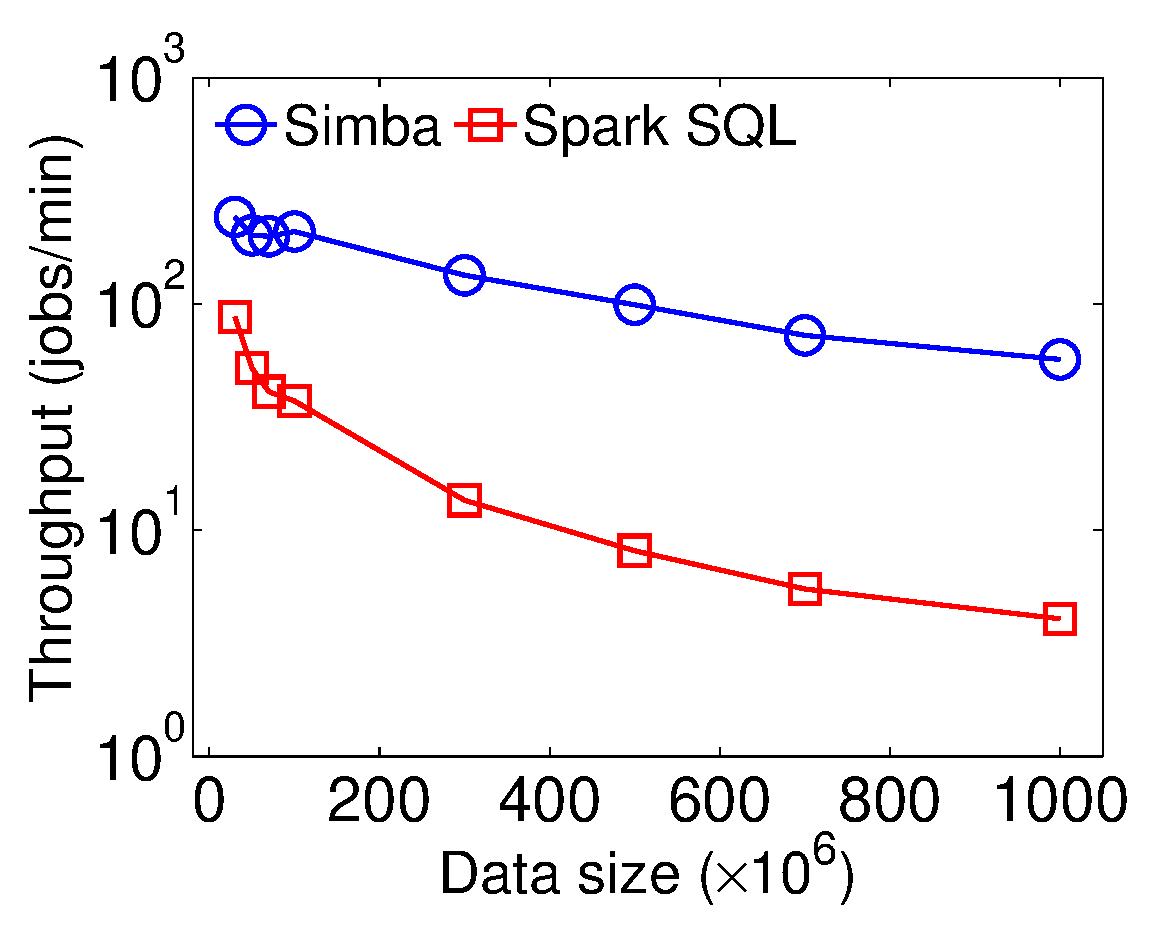
\includegraphics[width=1.55in]{figs/exp/osm_rect_datasize_throughput}
		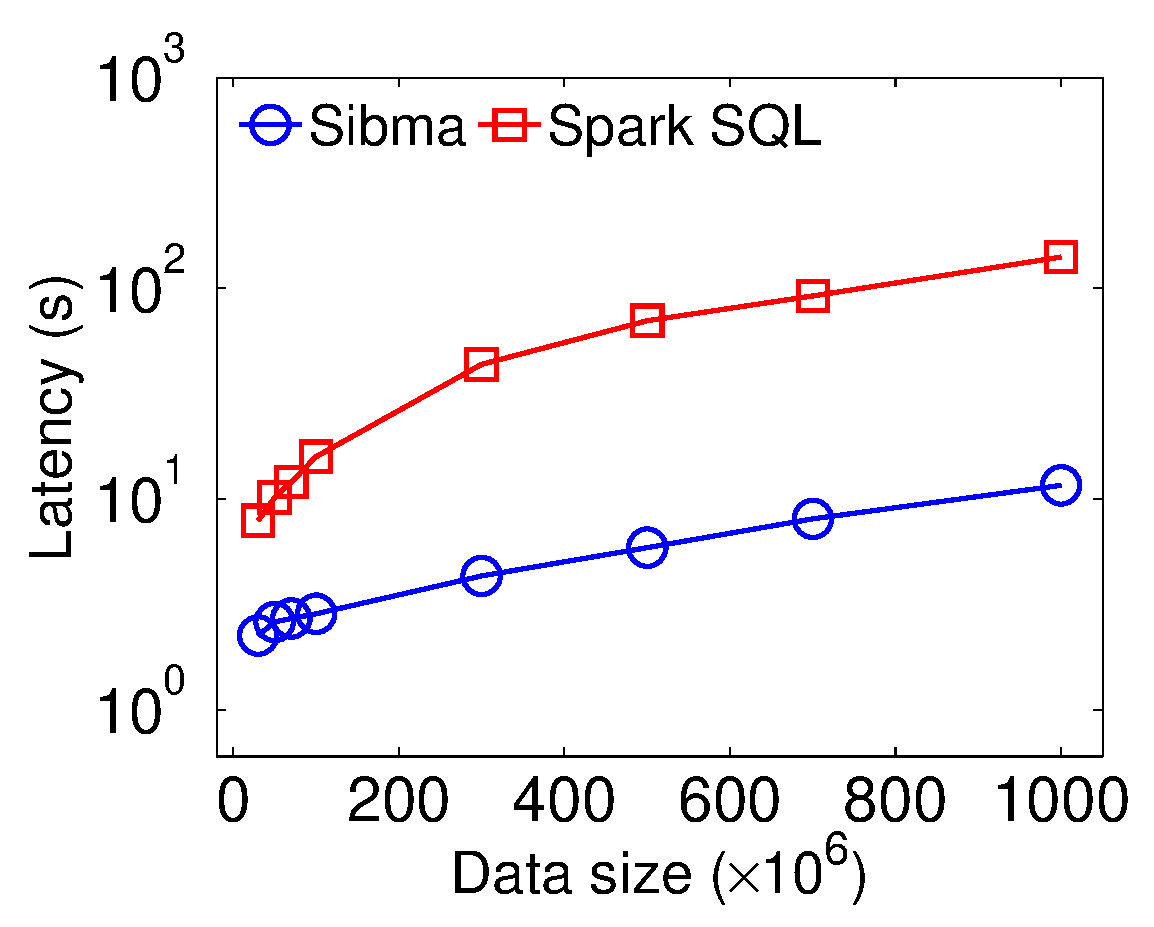
\includegraphics[width=1.55in]{figs/exp/osm_rect_datasize_latency}
	} \vspace{5mm}

	\subfigure[Effect of query area size (percentage of total area).]{
		\label{fig:osm_rect_rate}
		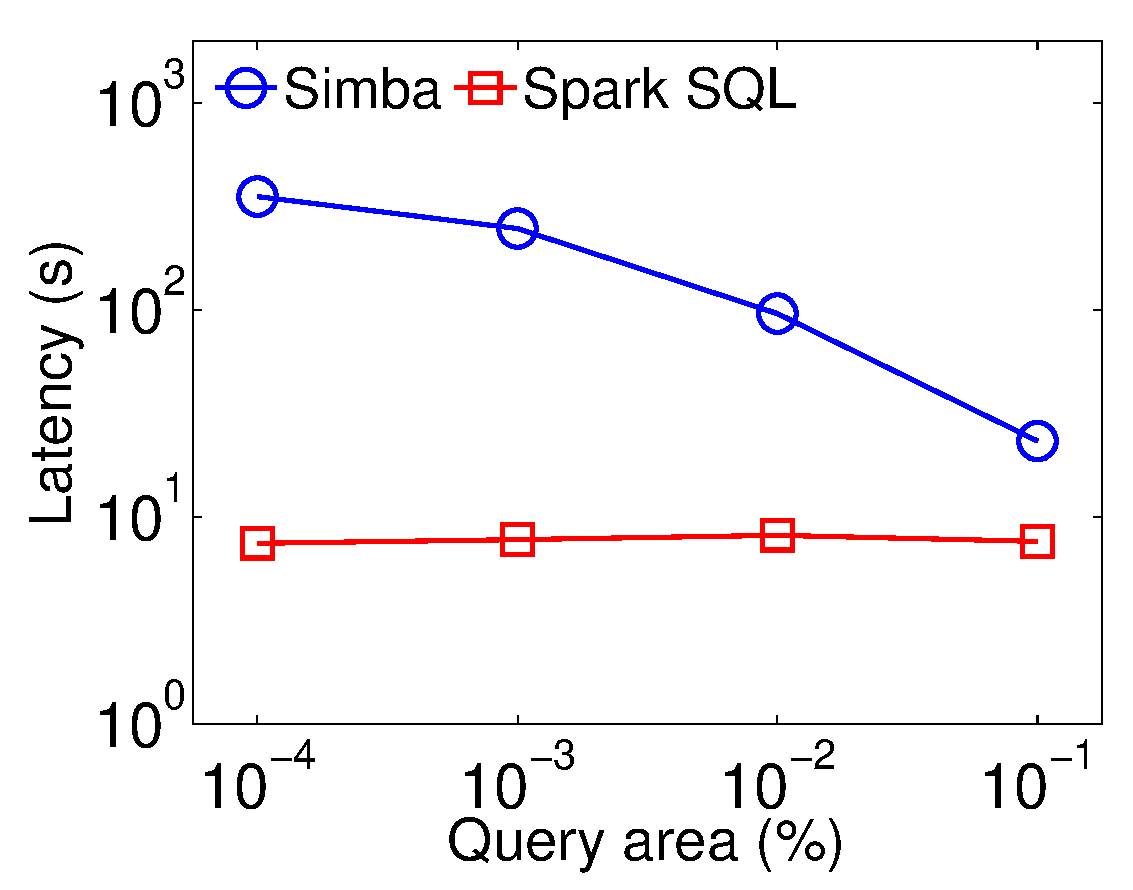
\includegraphics[width=1.55in]{figs/exp/osm_rect_rate_throughput}
		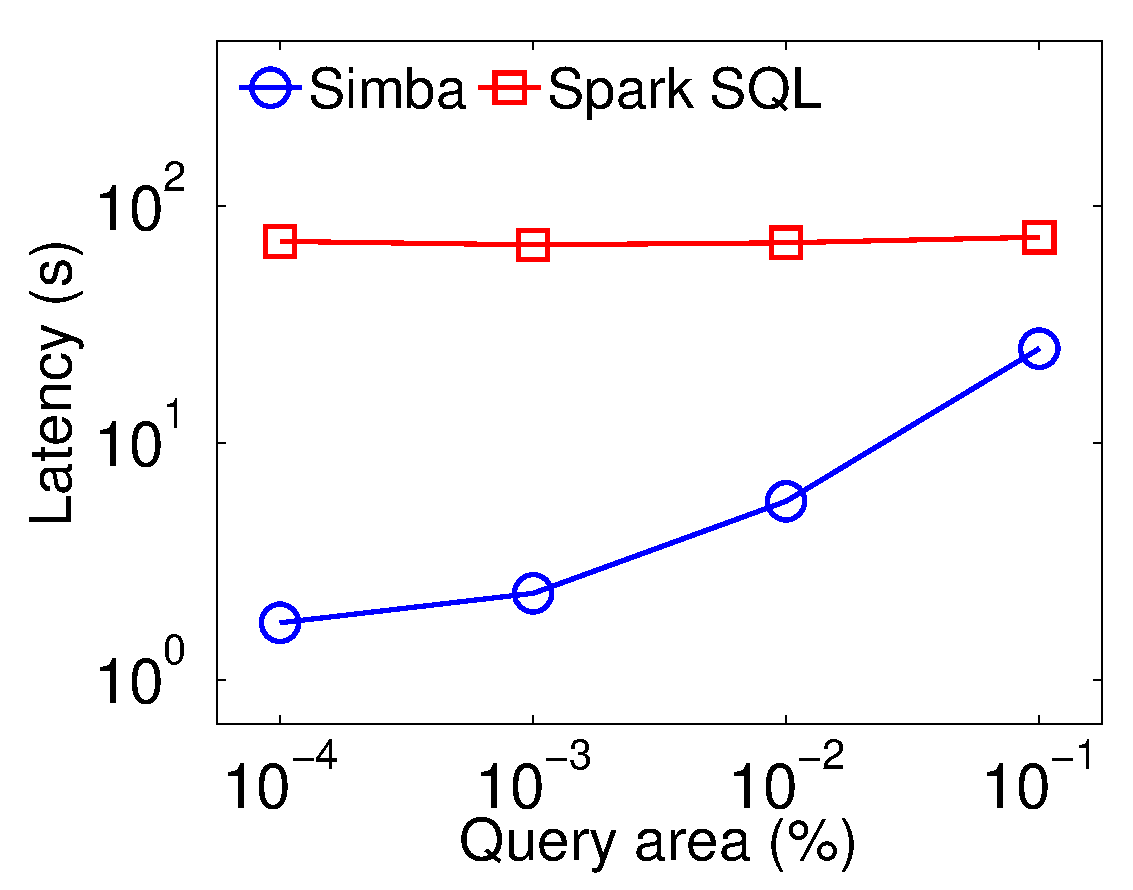
\includegraphics[width=1.55in]{figs/exp/osm_rect_rate_latency}
	} %\vspace{5mm}
	% \subfigure[Effect of partition size (number of records per partition).]{
	% 	\label{fig:osm_rect_partsize}
	% 	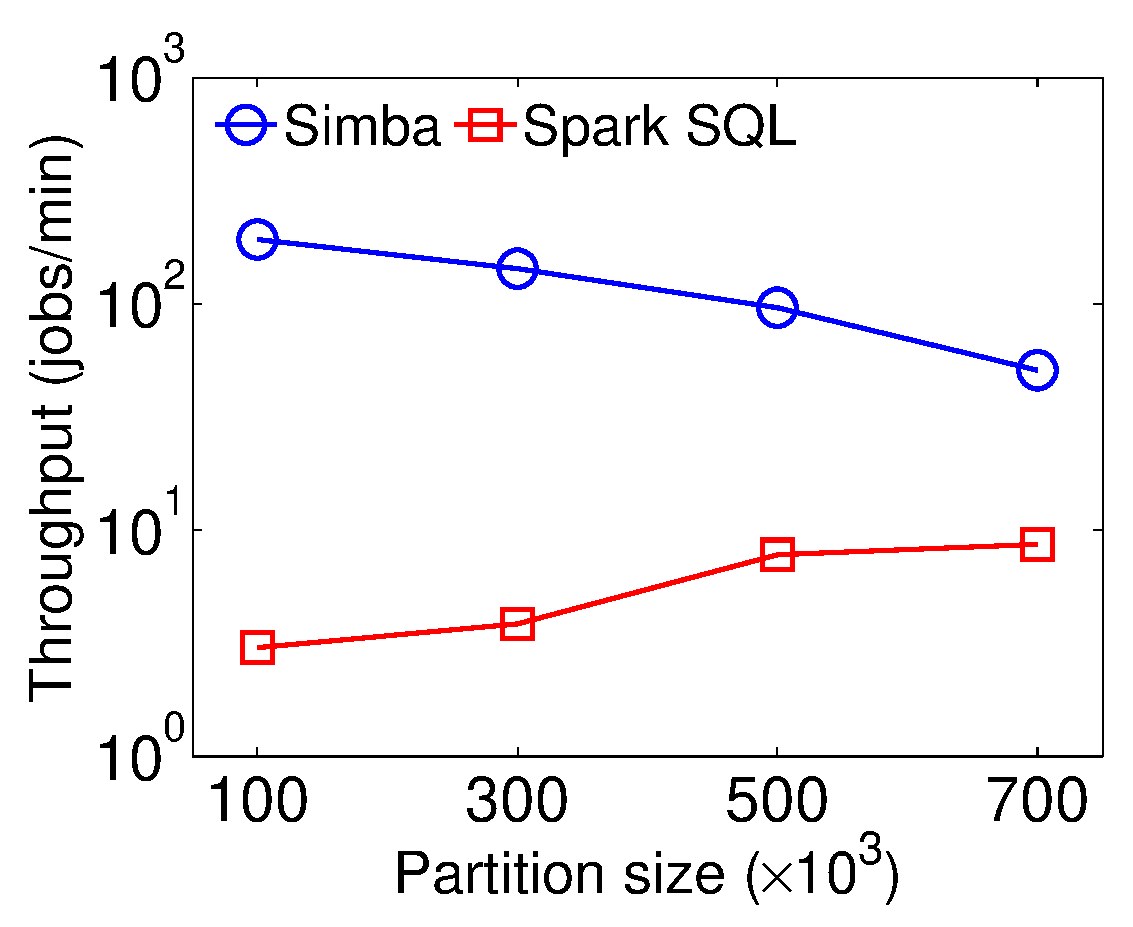
\includegraphics[width=1.55in]{figs/exp/osm_rect_partsize_throughput}
	% 	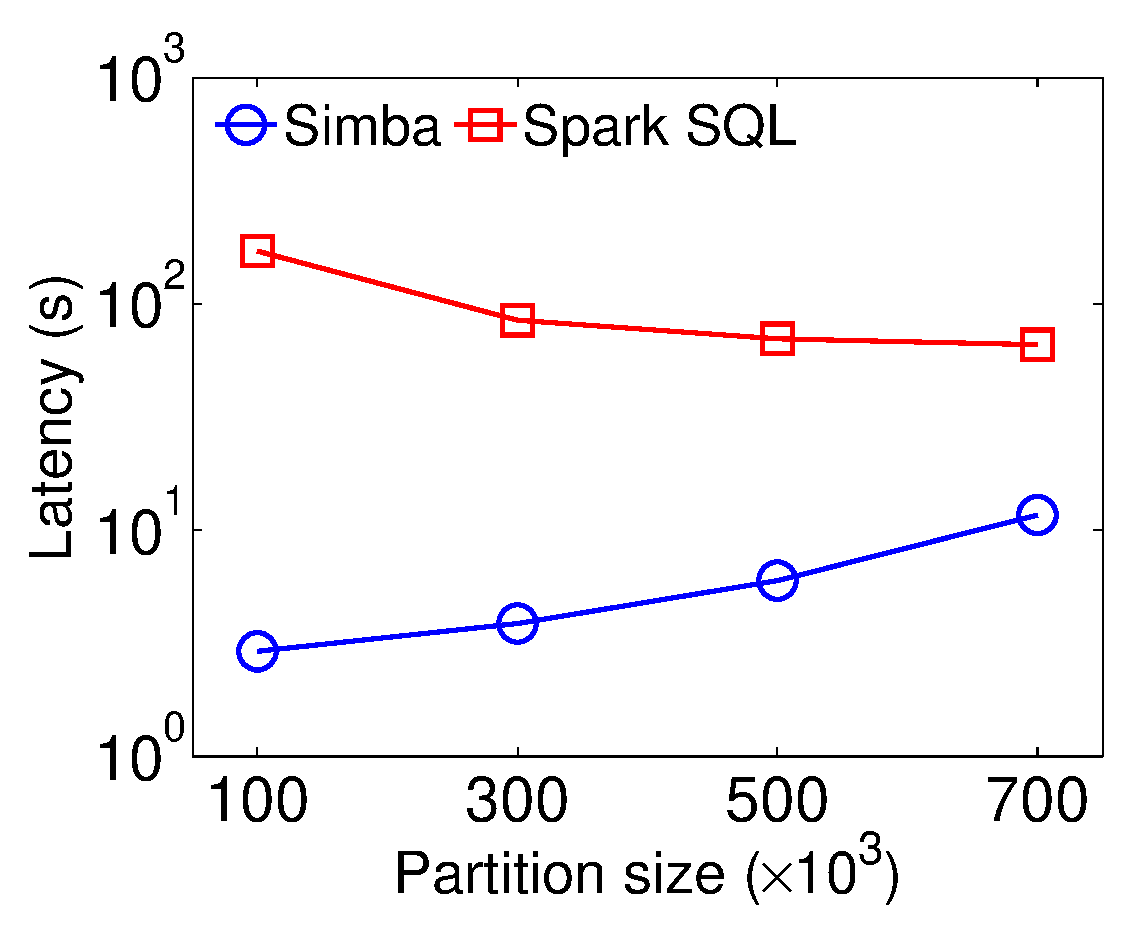
\includegraphics[width=1.55in]{figs/exp/osm_rect_partsize_latency}
	% }
	\caption{Range query performance on OSM.}
	\label{fig:range}\vspace{-5mm}
\end{figure}

\Paragraph{Range queries.}
Figure \ref{fig:range} shows the performance of range queries in both
engines using the OSM data set. Queries are centered at random points
sampled from the input data. As a result, the query workload fits well
with the distribution of the data, where dense areas will be queried
with higher probabilities.

Figure \ref{fig:osm_rect_datasize} shows that \name outperforms Spark
SQL by about one order of magnitude on both query throughput and query
latency.  The performance of both \name and Spark SQL drops when data
size increases while that of \name drops much slower, which implies
\name has much better scalability. This is because of spatial index
and spatial-aware optimization in \name: larger data size does lead to
more partitions to process and larger output size, but it also implies
potentially more pruning power from its indexes and optimizer. In
contrast, Spark SQL has to scan the whole table regardless.

Figure \ref{fig:osm_rect_rate} shows how throughput and latency are
influenced by the size of the query area. As the query area enlarges,
performance of \name becomes closer to that of Spark SQL. The reason
for this is the result size becomes very large and there is less
optimization opportunities for \name's query optimizer. Spark SQL's
query performance is {\em hardly} affected by the size of the query
area, since it has to scan the whole table regardless.

\Paragraph{$k$NN queries.}
Figure \ref{fig:knn} shows the performance of $k$NN queries on Spark
SQL and \name, using the OSM data set, where query points are randomly
sampled from the input data.
Figure \ref{fig:osm_knn_datasize} measures system throughput and query
latency when increasing the data size from 30 million to 1 billion
records. \name achieves one to two orders of magnitude better
performance on both metrics. Spark SQL's performance drops
significantly as data becomes larger, since it requires scanning the
whole table for a $k$NN query, while \name's performance is almost not
affected by the data increase since regardless of the data size, \name
is able to narrow down quickly to just a few RDD partitions that may
contain the $k$NNs.

Next, using the default data size which is 500 million records, we
study the impact of $k$. As $k$ varies from $1$ to $50$ in Figure
\ref{fig:osm_knn_k}, \name maintains a speedup of two orders of
magnitude. Both \name and Spark SQL's performance are not really
affected by $k$: Spark SQL needs to scan the data regardless of $k$
values; whereas \name's performance will not change much when the
change in $k$ is much smaller compared to the partition size.


\begin{figure}[!t]
	\centering
	\subfigure[Effect of data size.]{
		\label{fig:osm_knn_datasize}
		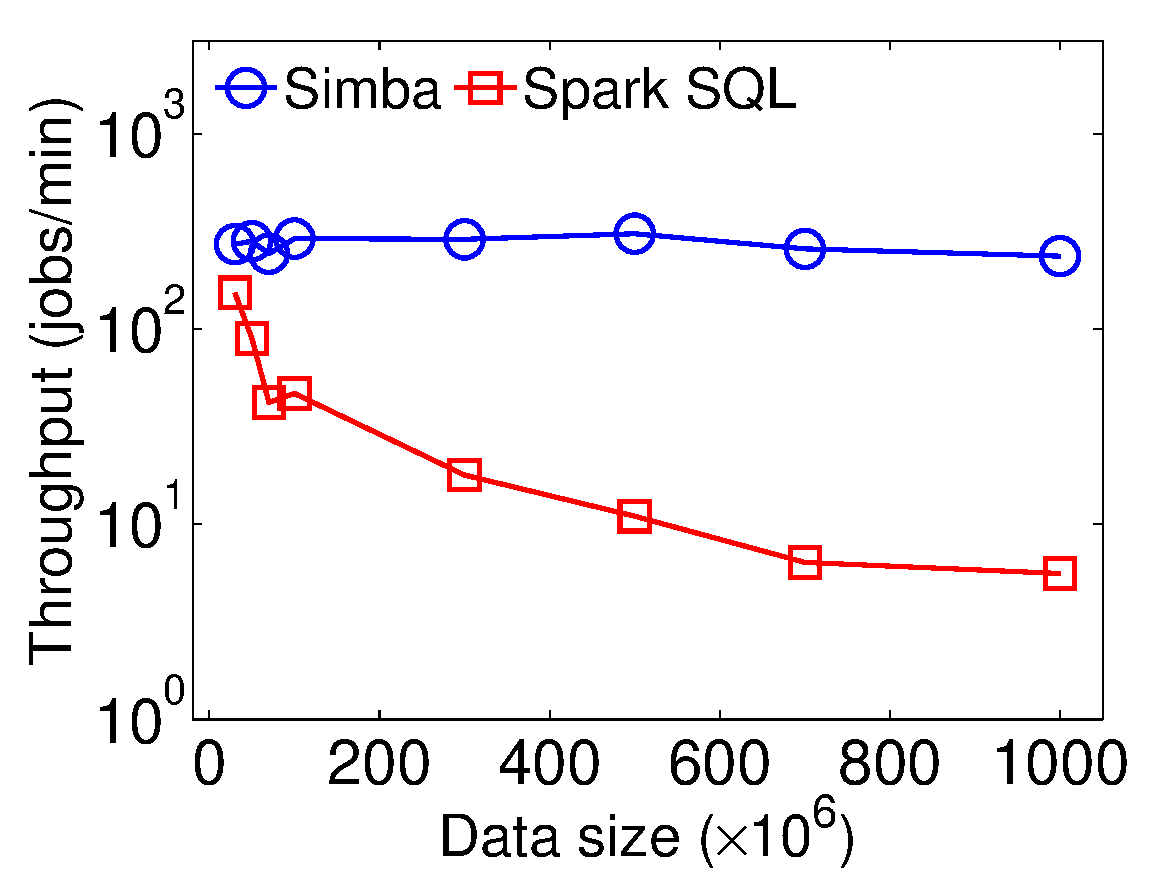
\includegraphics[width=1.55in]{figs/exp/osm_knn_datasize_throughput}
		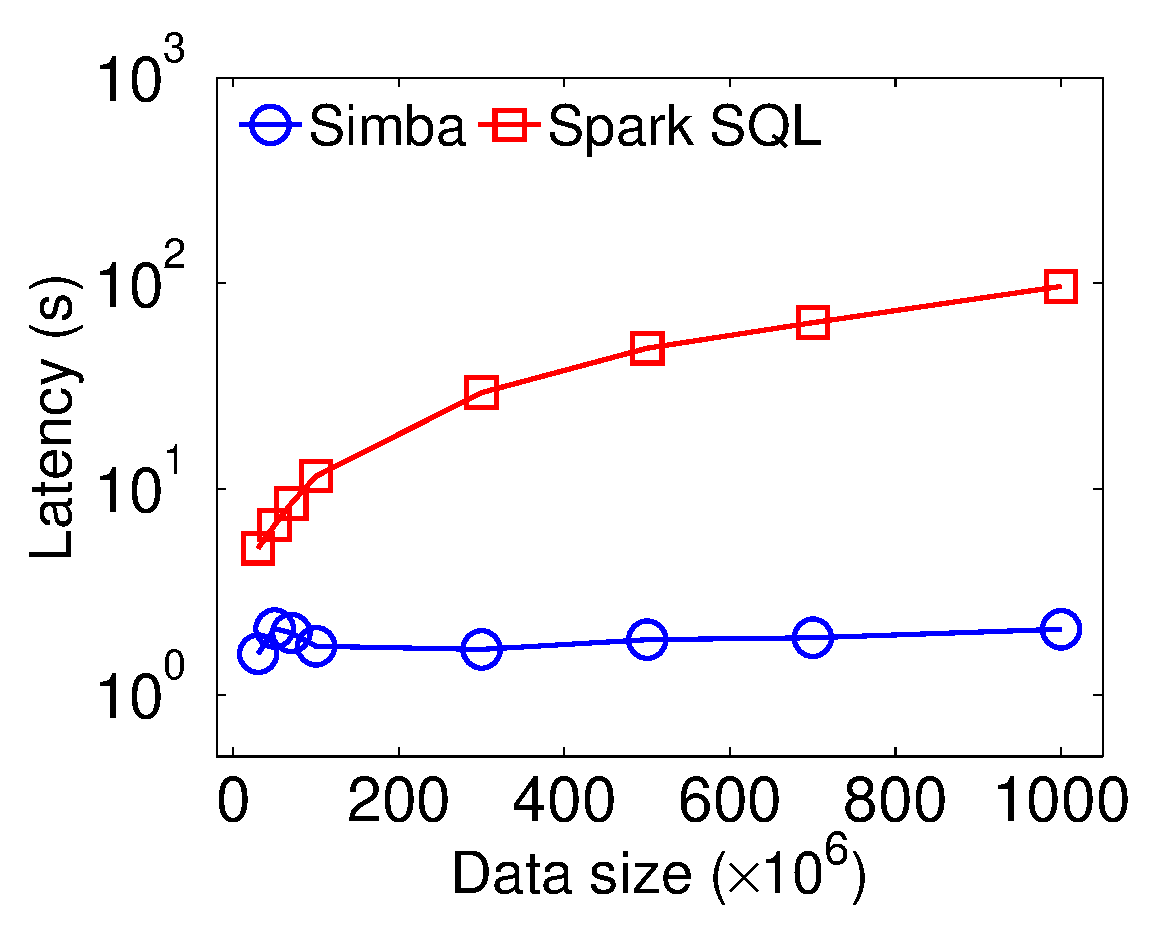
\includegraphics[width=1.55in]{figs/exp/osm_knn_datasize_latency}
	} \vspace{4mm}

	\subfigure[Effect of $k$.]{
		\label{fig:osm_knn_k}
		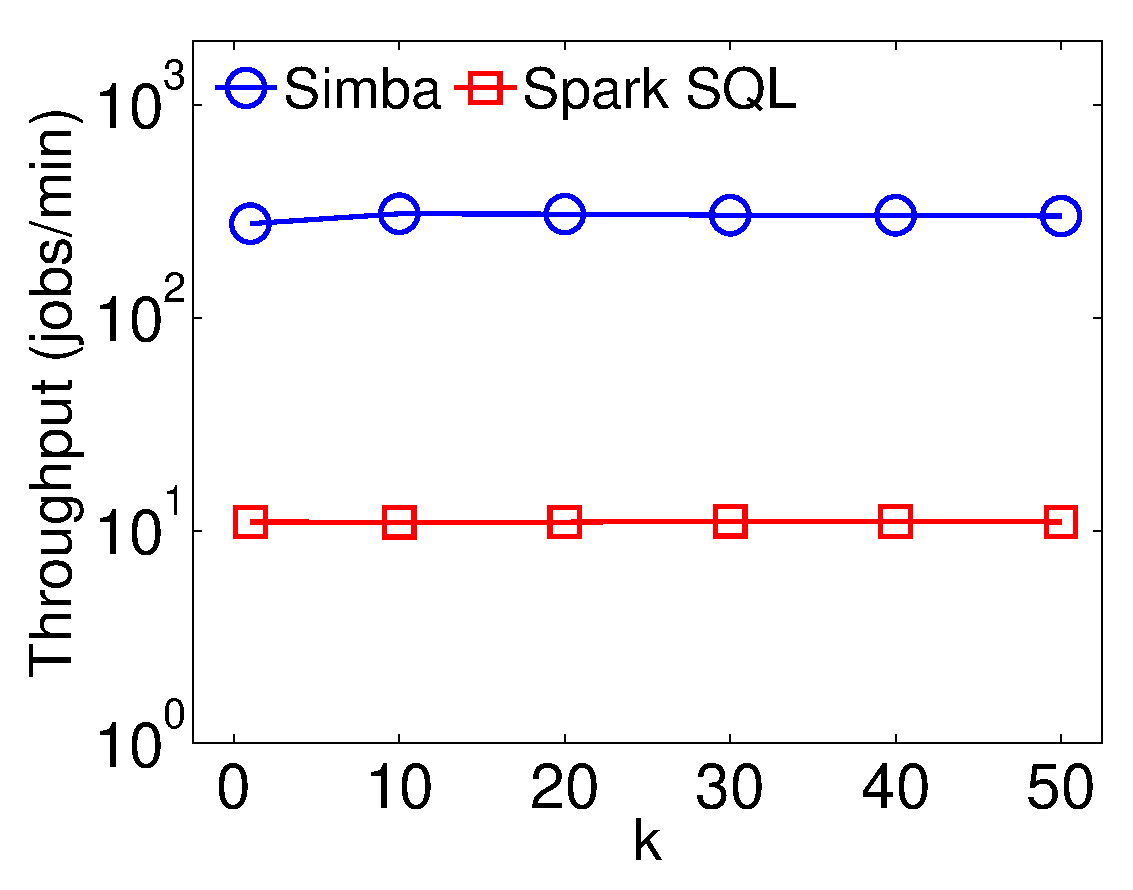
\includegraphics[width=1.55in]{figs/exp/osm_knn_k_throughput}
		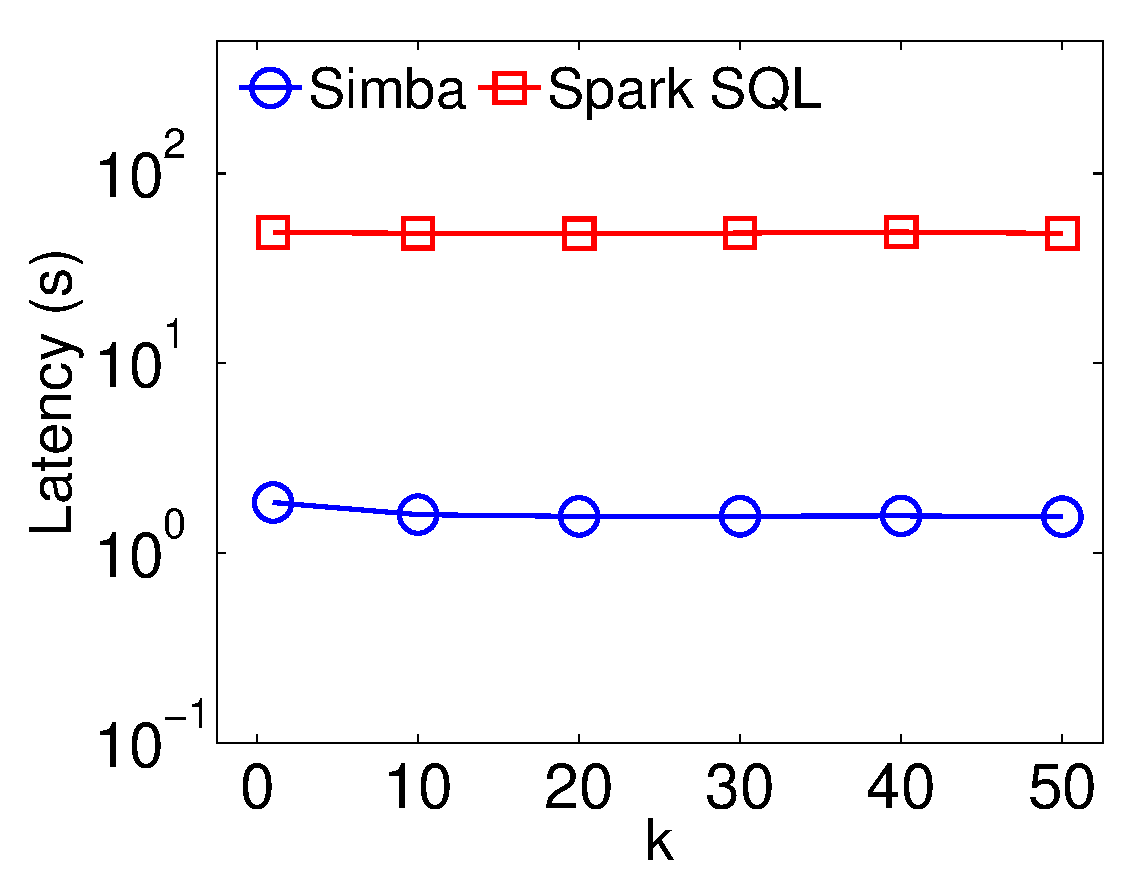
\includegraphics[width=1.55in]{figs/exp/osm_knn_k_latency}
	} % \vspace{4mm}

	% \subfigure[Effect of partition size (number of records per partition).]{
	% 	\label{fig:osm_knn_partsize}
	% 	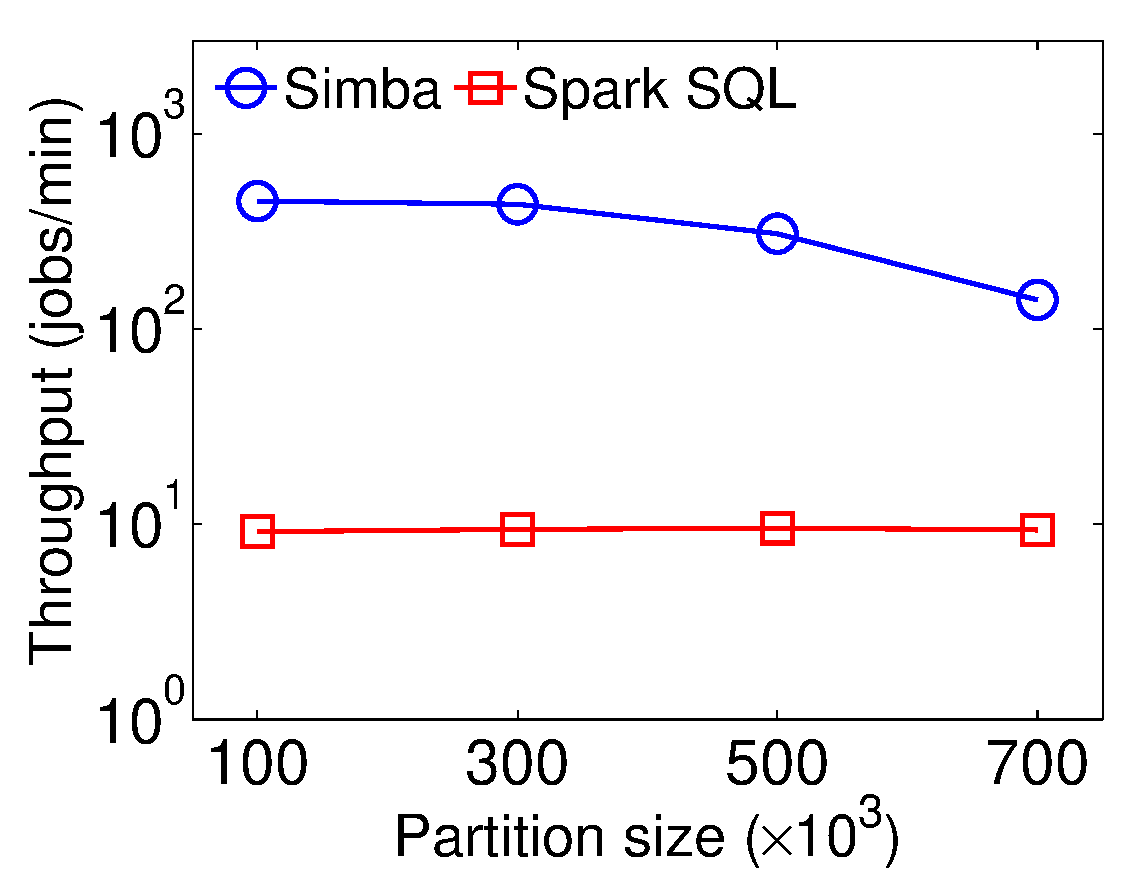
\includegraphics[width=1.55in]{figs/exp/osm_knn_partsize_throughput}
	% 	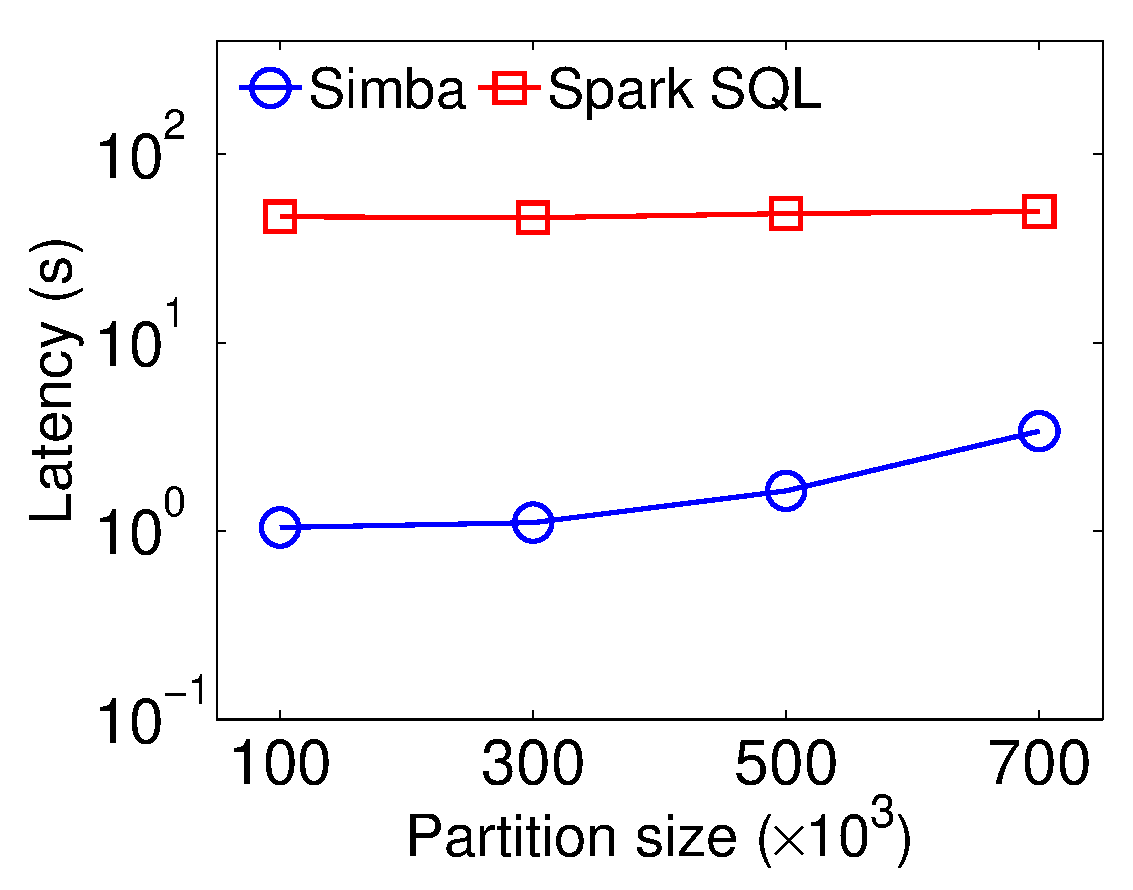
\includegraphics[width=1.55in]{figs/exp/osm_knn_partsize_latency}
	% }\vspace{0mm}
	\caption{$k$NN query performance on OSM.}\vspace{-4mm}
	\label{fig:knn}
\end{figure}



\Paragraph{Distance join.}
Figure \ref{fig:disj} shows the results of the distance join
experiments, using two tables sampled from OSM (each is 3 million
records). We tried expressing and running a distance join as an
$\theta$-join in Spark SQL (an example was shown in Section
\ref{sub:disjoin}). However, {\em it did not finish in 10 hours when
  joining two tables of only 1 million records, and crashed, due to
  the expensive cartesian product it has to perform}.


\begin{figure}[!t]
	\subfigure[Effect of data size.]{
		\label{fig:osm_disj_datasize}
		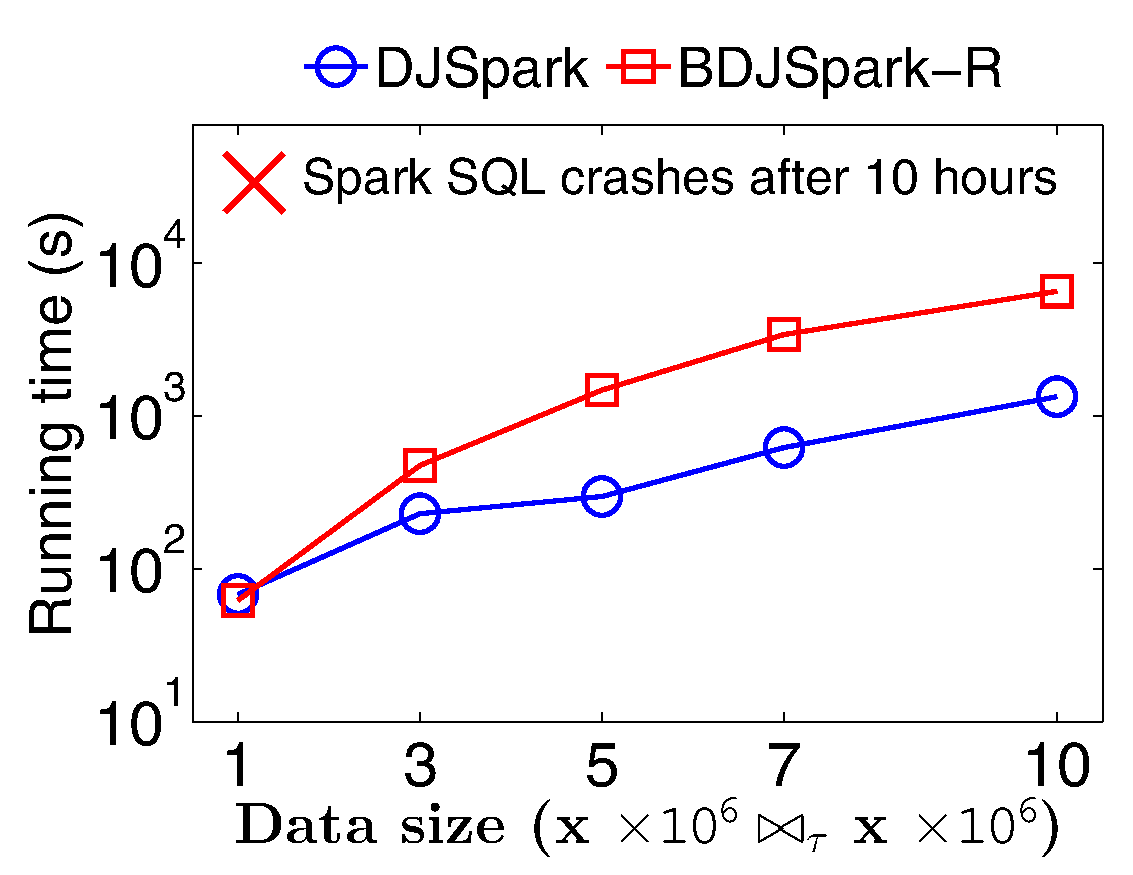
\includegraphics[width=1.55in]{figs/exp/osm_disj_datasize}
	} %\vspace{6mm}
	\subfigure[Effect of $\tau$.]{
		\label{fig:osm_disj_rate}
		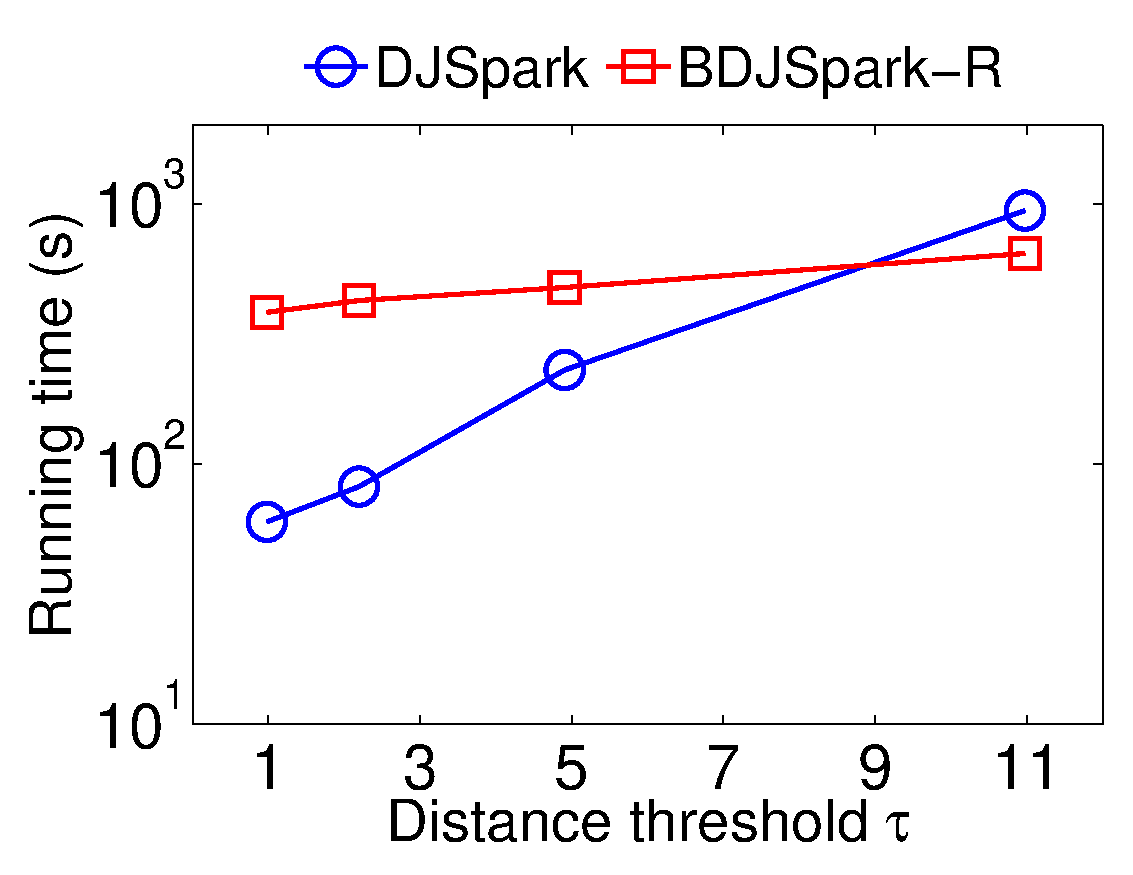
\includegraphics[width=1.55in]{figs/exp/osm_disj_rate}
	} %\vspace{6mm}
	%\centering
	%\subfigure[Effect of expected partition size]{
	%	\label{fig:osm_disj_partsize}
	%	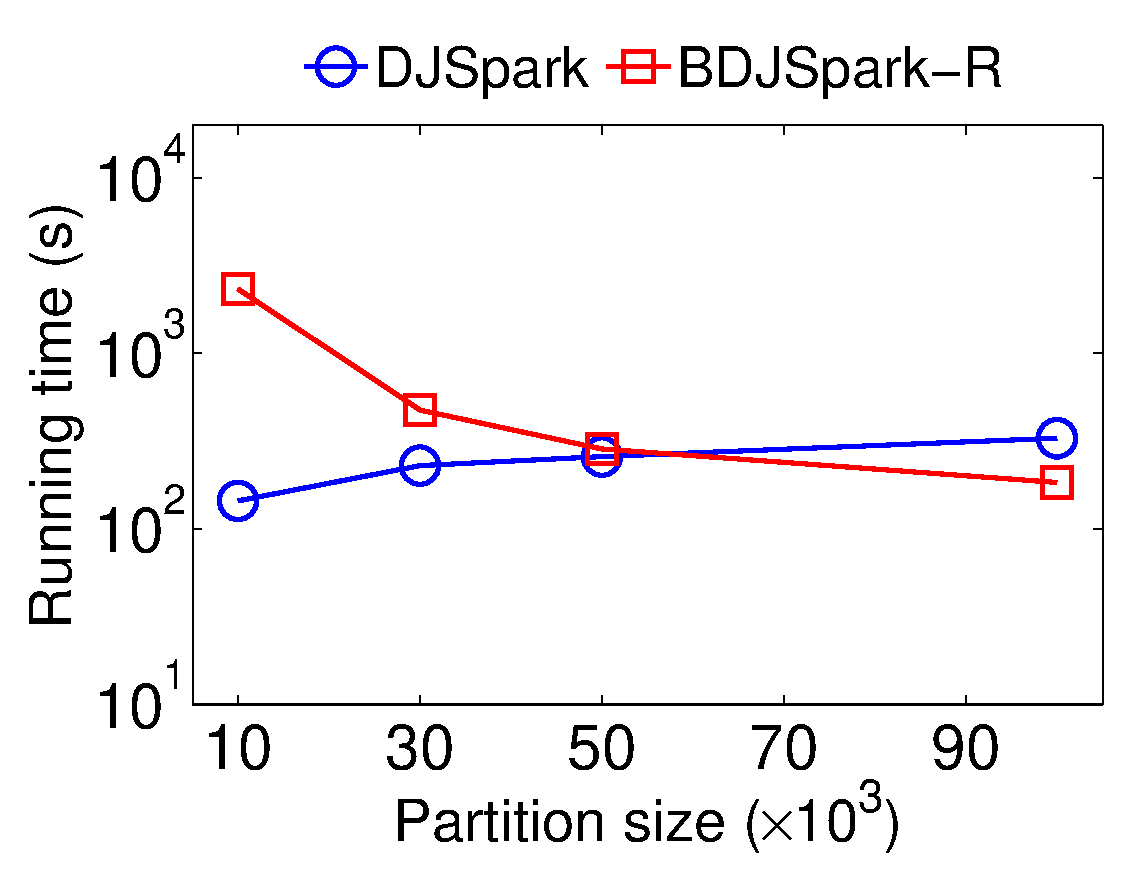
\includegraphics[width=1.74in]{figs/exp/osm_disj_partsize}
  %} \vspace{-6mm}
	\caption{Distance join performance on OSM.}
	\label{fig:disj}\vspace{-3mm}
\end{figure}


\begin{figure}[!t]
	\subfigure[Effect of data size.]{
		\label{fig:osm_knnj_datasize}
		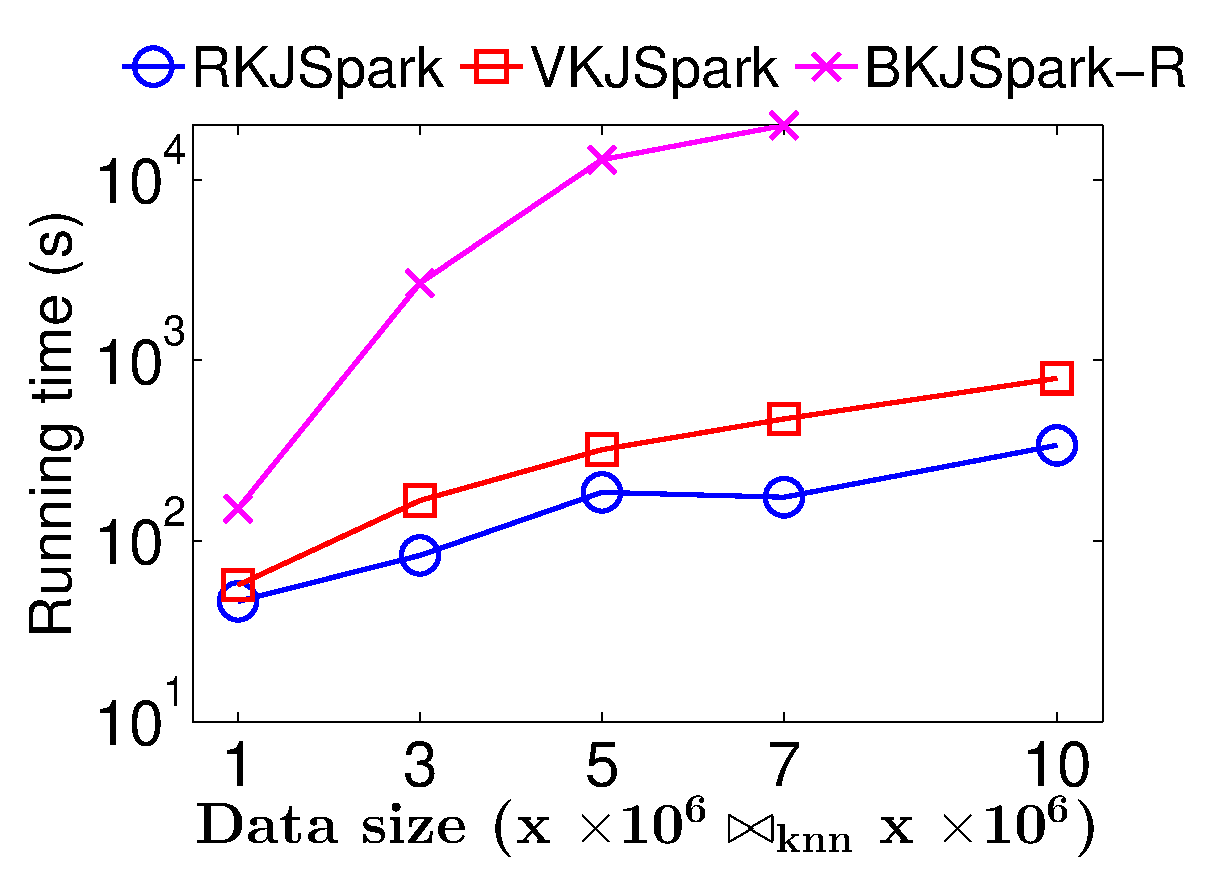
\includegraphics[width = 1.55in]{figs/exp/osm_knnj_datasize}
	} %\vspace{6mm}
	\subfigure[Effect of $k$.]{
		\label{fig:osm_knnj_k}
		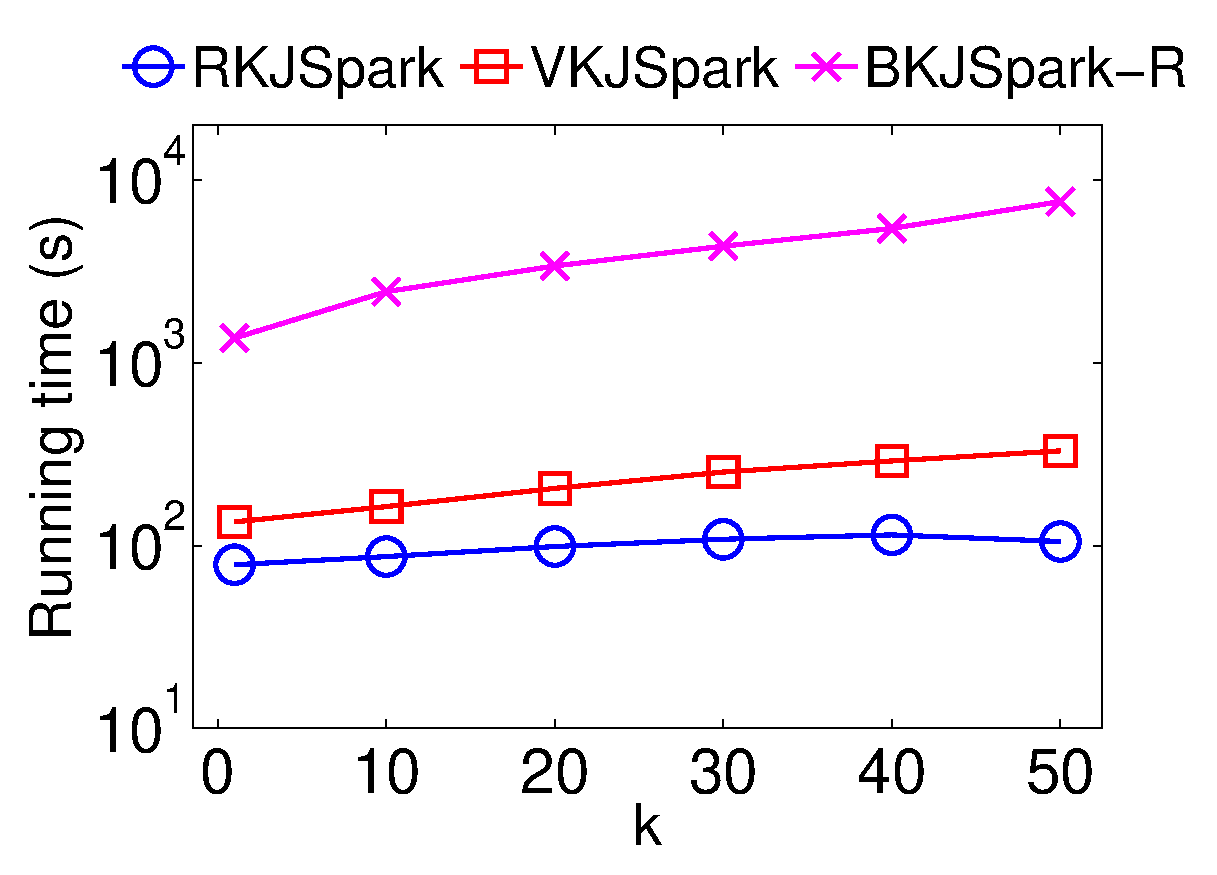
\includegraphics[width = 1.55in]{figs/exp/osm_knnj_k}
	} %\vspace{6mm}
	%\centering
	%\subfigure[Effect of expected partition size]{
	%	\label{fig:osm_knnj_partsize}
	%	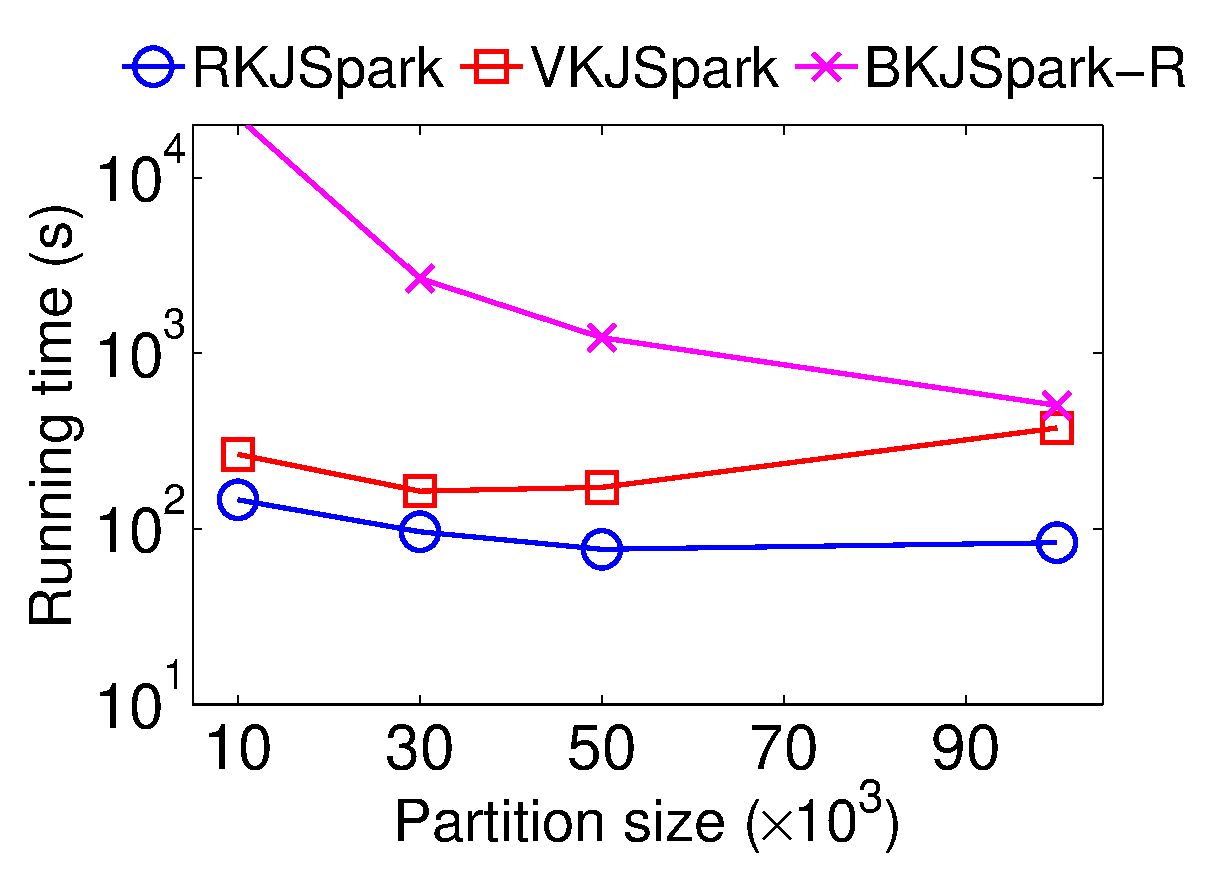
\includegraphics[width=1.74in]{figs/exp/osm_knnj_partsize}
	%} \vspace{-5mm}
	\caption{$k$NN join performance on OSM.}
	\label{fig:knnj}\vspace{-4mm}
\end{figure}


For \name, we compared the algorithm DJSpark as introduced in Section
\ref{sub:disjoin} and a nested loop join approach using R-trees as
local indexes, termed as BDJSpark-R (a simple variation of BKJSpark-R
discussed in Section \ref{sub:knnjoin}; replacing each local $k$NN
join with a local distance join).

% \dong{We did not introduce the nested-loop version (with R-Tree) and
%   the hash join version for distance joins in this paper. I
%   temporarily term the nested-loop version as BDJSpark-R, and the
%   hash-join version as HDJSpark.}

Naturally, the cost of both algorithms increase with larger input size
(Figure \ref{fig:osm_disj_datasize}) and larger distance threshold
(Figure\ref{fig:osm_disj_rate}). Nevertheless, DJSpark is always more
efficient than the baseline method BDJSpark-R, unless the threshold
grows to a relatively large value (say $x=11$ in this case; roughly
1\% of the space). % (\feifei{specify this distance value
  % and the average points retrieved}).

%In Figure \ref{fig:osm_disj_partsize}, as expected partition size grows,
%running time of DJSpark and HDJSpark increases slightly as the pruning
%power of the global join phase reduces when partition granularity is
%decreasing. In contrast, BDJSpark-R becomes faster since fewer local
%join tasks are required for processing.

\Paragraph{$k$NN join.}
It is {\em impossible to express $k$NN join in Spark SQL}, unless
using $N$ union statements where $N$ is the number of records in the
first input table, which is clearly not a practical solution for large
tables. Hence, we focused on comparing different $k$NN join algorithms
in \name.

Figure \ref{fig:knnj} shows the performance over OSM data (default is
$3$ million records in each input table and $k=10$). clearly, RKJSpark
shows the best performance and best scalability (wrt both data size
and $k$). As an example, for a $k$NN join between two 5 million
records tables, RKJSpark join is 3x faster than VKJSpark and 70x
faster than BKJSpark-R. Note that BKJSpark-R strictly dominates
BKJSpark-N, hence, the later is omitted.

% Figure \ref{fig:osm_knnj_k} presents the effect of $k$ on different
% algorithms. With increasing of $k$, running time of BKJSpark-R and
% VKJSpark join grows faster than that of RKJSpark. This is mainly
% because RKJSpark leverages the power of local indexes.

%In Figure \ref{fig:osm_knnj_partsize}, as expected partition size
%increases, BKJSpark-R and RKJSpark become faster since fewer local
%join tasks are required for processing.  VKJSpark runs slightly slower
%when expected partition size increases as the power of its pruning
%bounds weakens with the decreasing on pivot number.

\begin{figure}[t!]
	\centering
	% \subfigure[Synthetic]{
	% 	\label{fig:synthetic_rect_dimension}
	% 	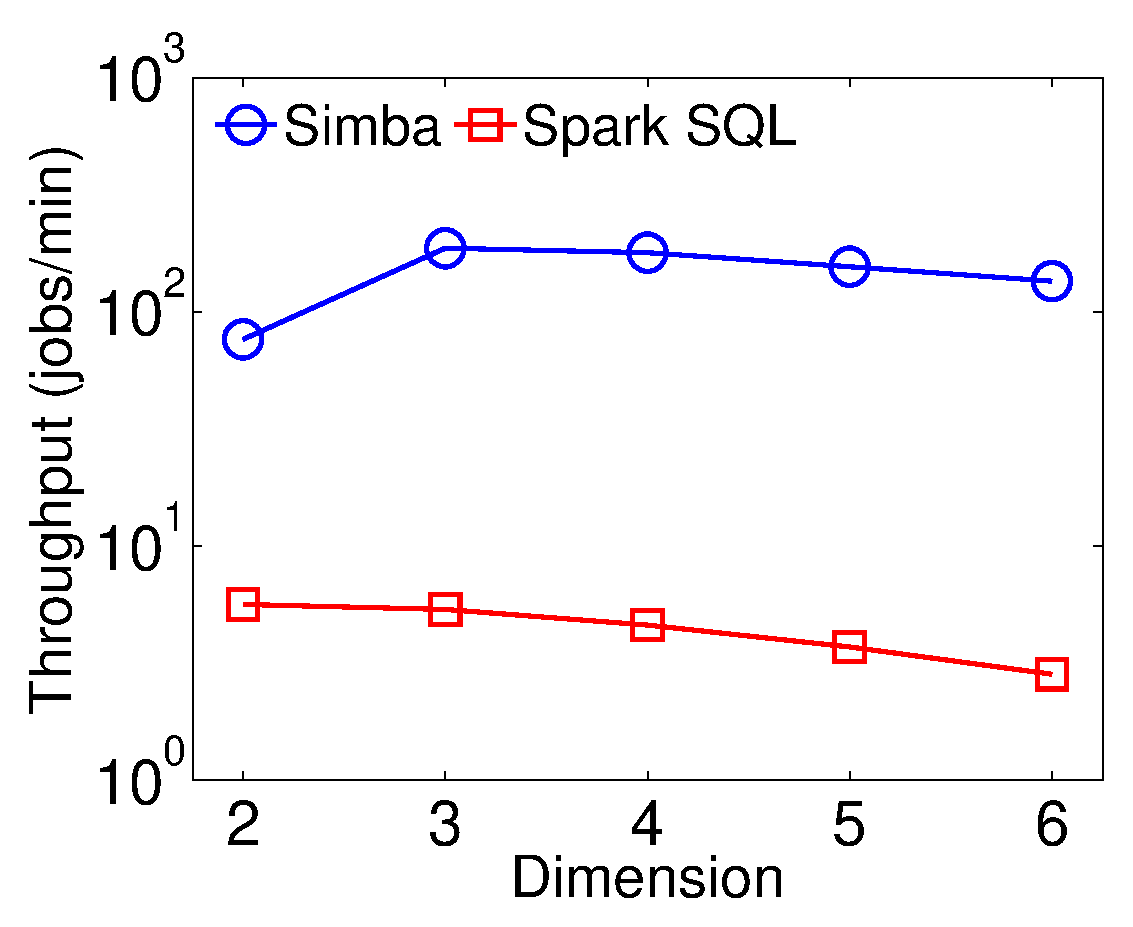
\includegraphics[width=1.55in]{figs/exp/gaussian700m_rect_dimension_throughput}
	% 	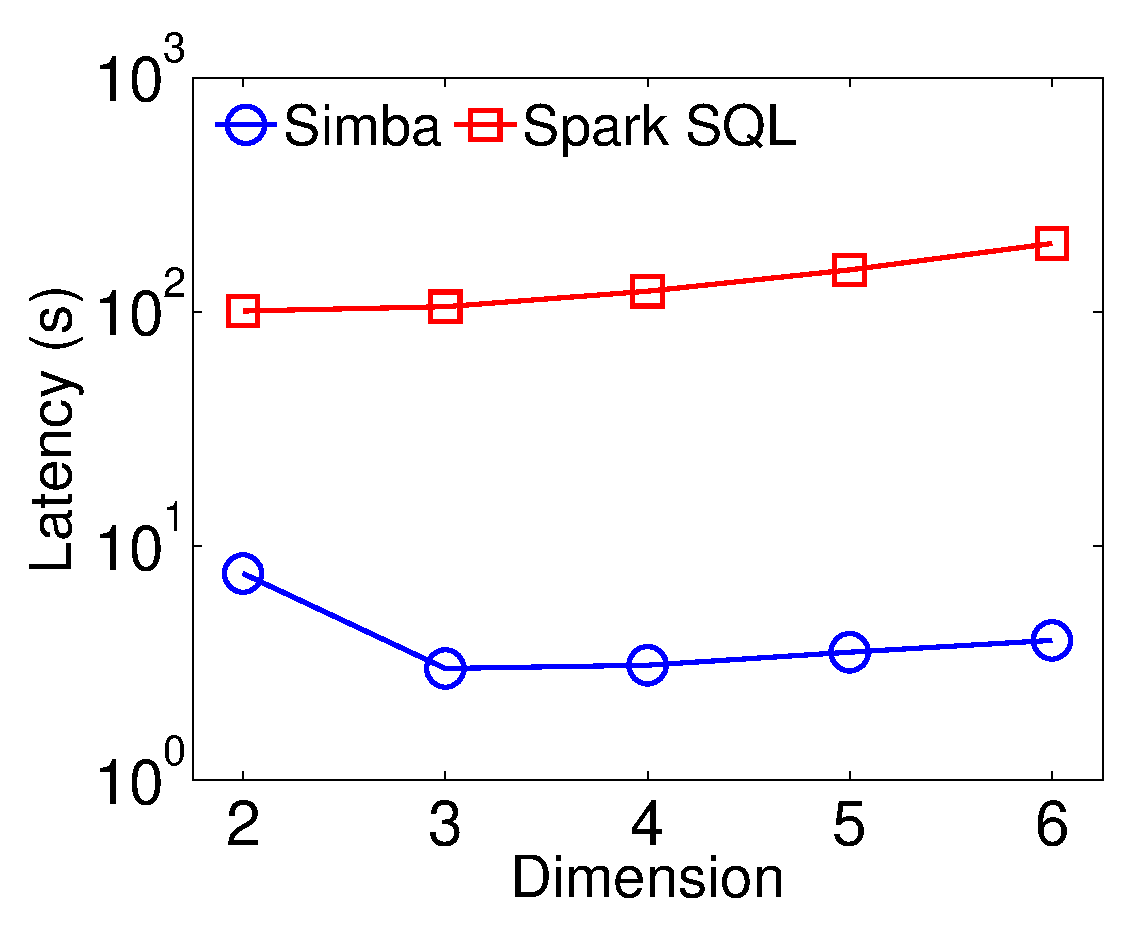
\includegraphics[width=1.55in]{figs/exp/gaussian700m_rect_dimension_latency}
	% }
	
	\subfigure[Throughput] {
		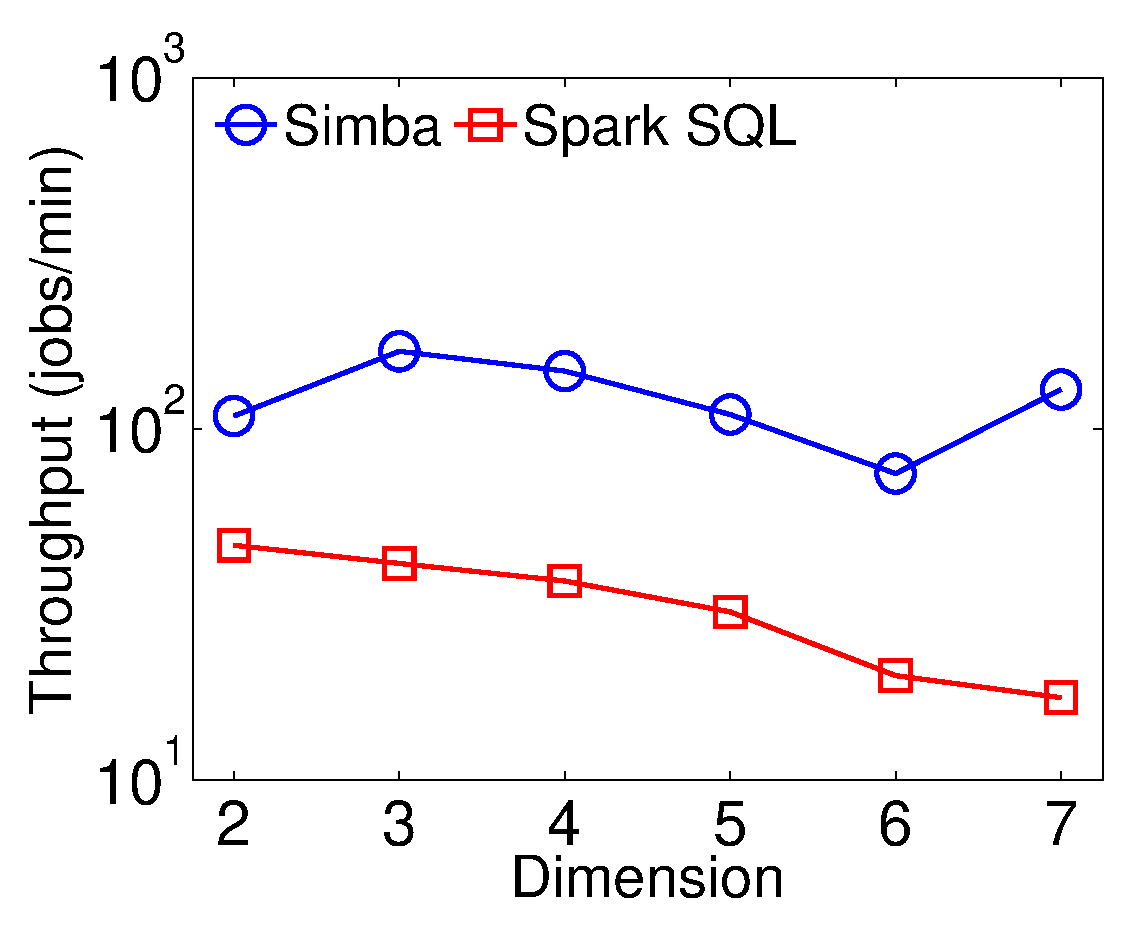
\includegraphics[width=1.55in]{figs/exp/gdelt_rect_dimension_throughput}
		\label{fig:gdelt_rect_dim_throughput}
	}
	\subfigure[Latency] {
		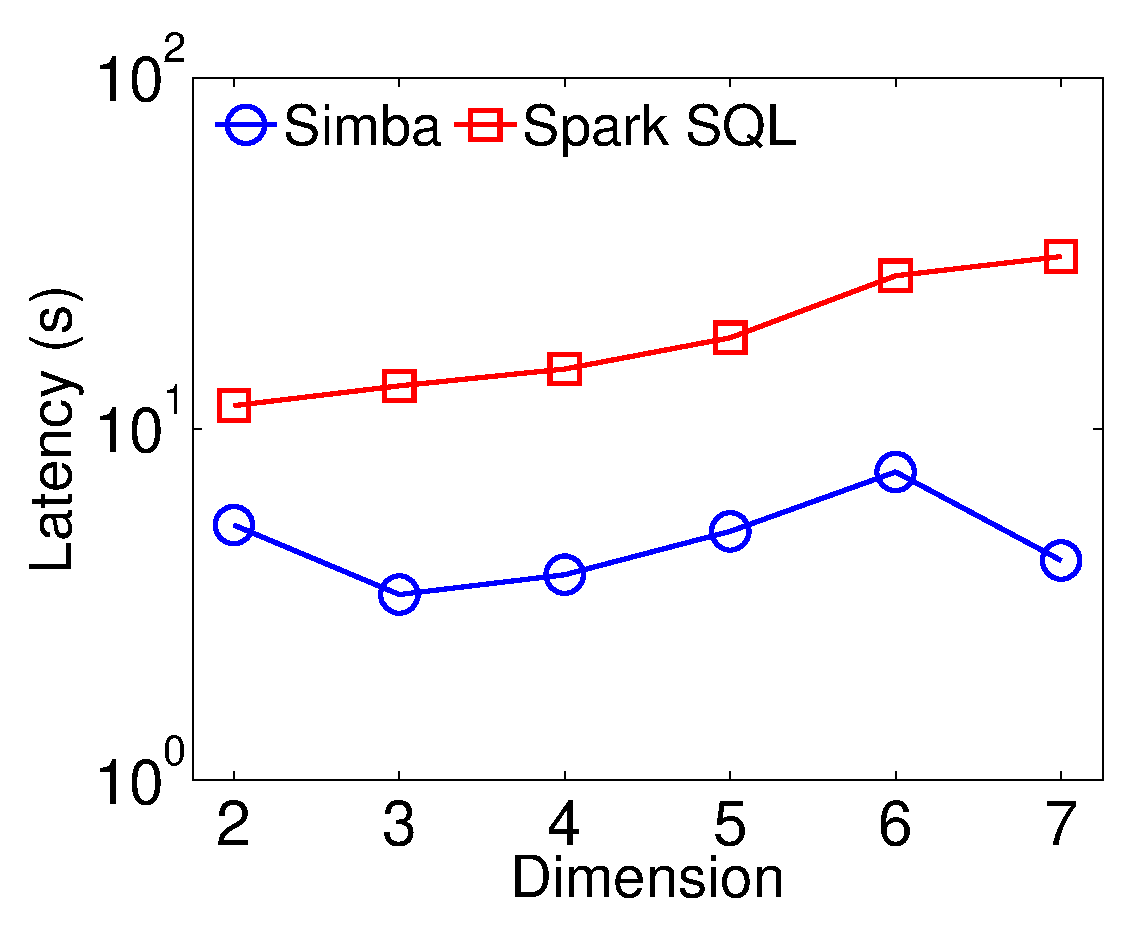
\includegraphics[width=1.55in]{figs/exp/gdelt_rect_dimension_latency}
		\label{fig:gdelt_rect_dim_latency}
	}
	%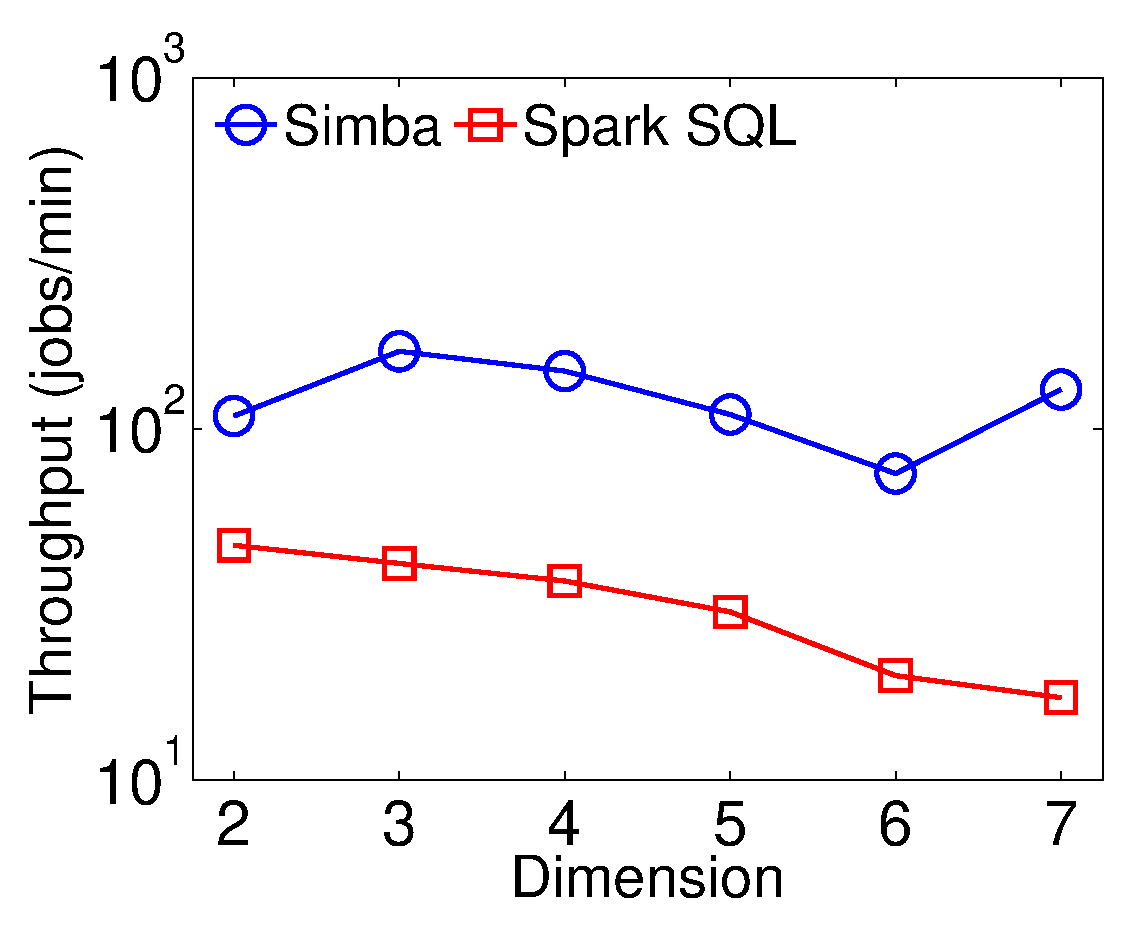
\includegraphics[width=1.55in]{figs/exp/gdelt_rect_dimension_throughput}
	%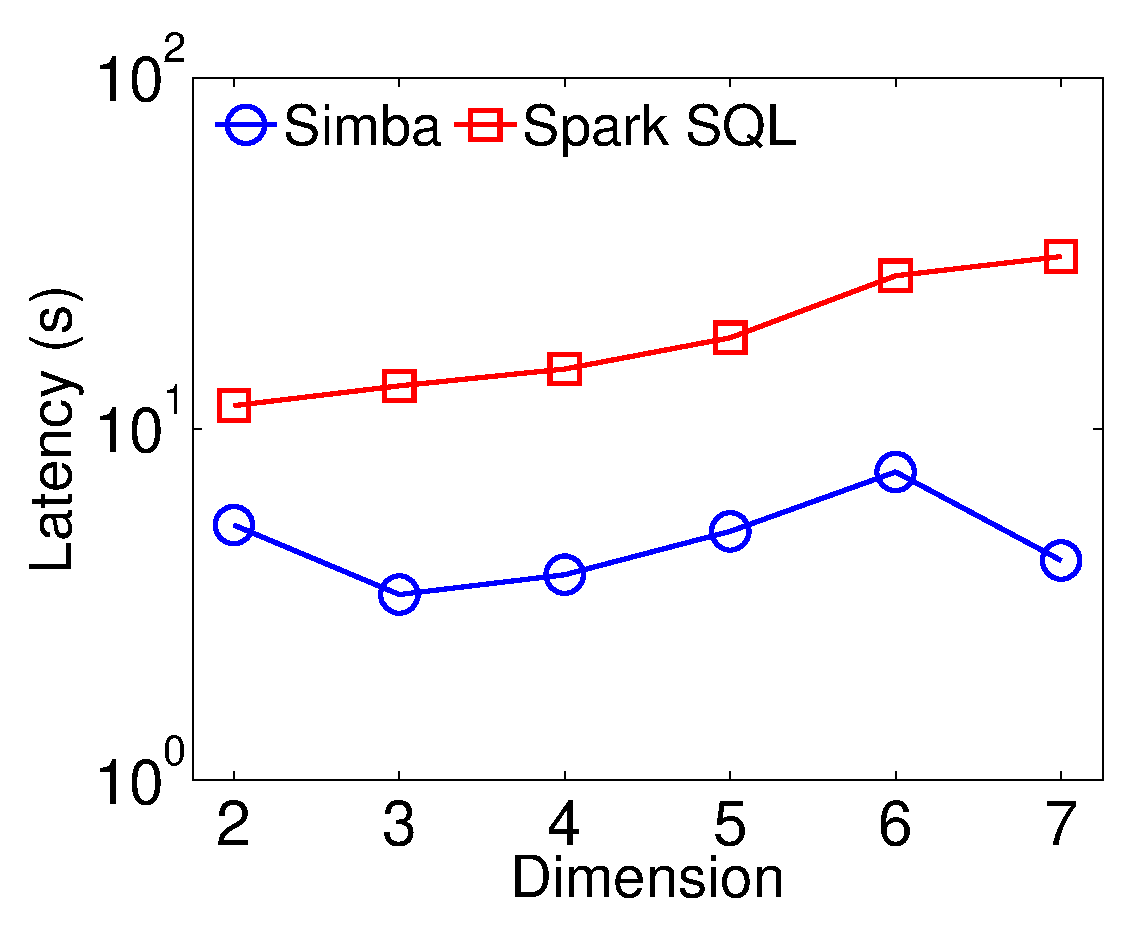
\includegraphics[width=1.55in]{figs/exp/gdelt_rect_dimension_latency}
	
	\caption{\small Range query performance vs. dimensionality on GDELT.}
	\label{fig:gdelt_rect_dimension}\vspace{-3mm}
\end{figure}

\begin{figure}[t]
	\centering
	% \subfigure[Synthetic]{
	% 	\label{fig:synthetic_knn_dimension}
	% 	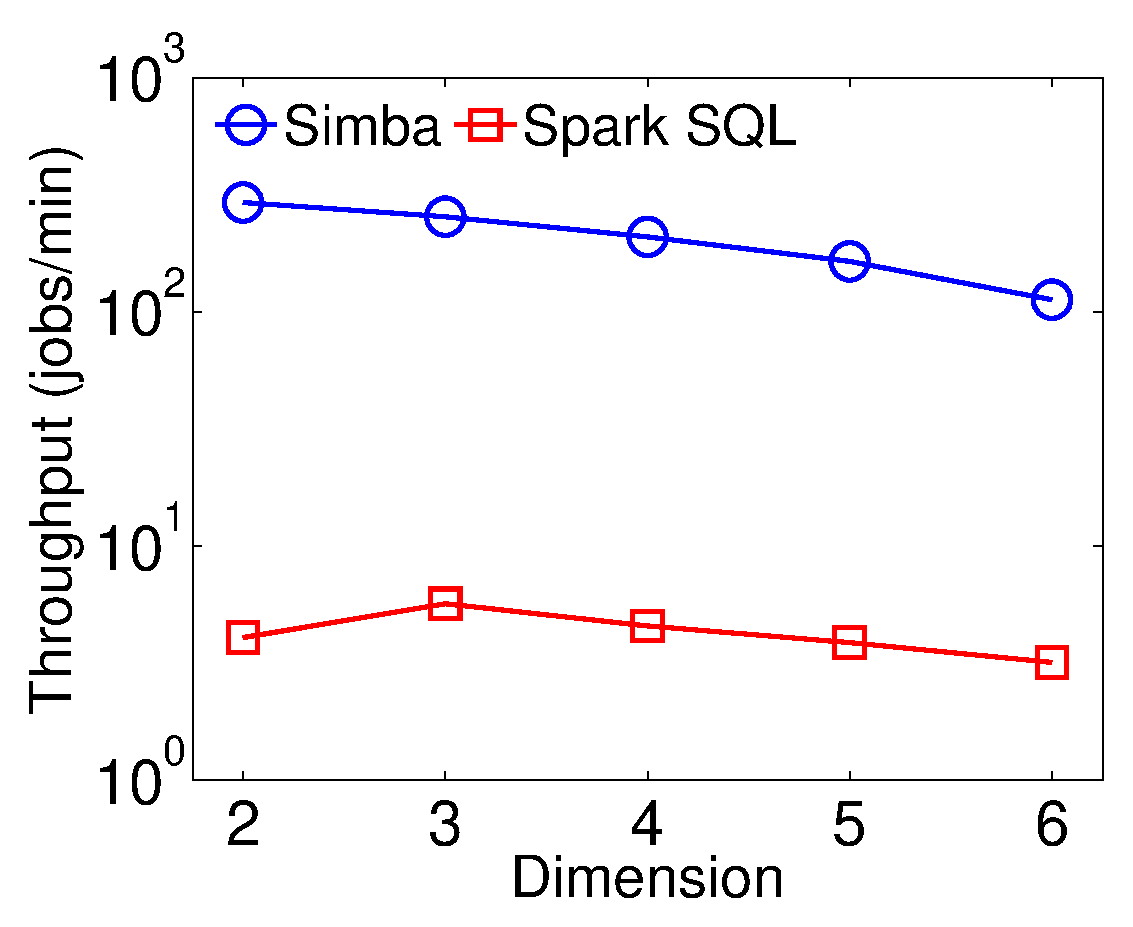
\includegraphics[width=1.55in]{figs/exp/gaussian700m_knn_dimension_throughput}
	% 	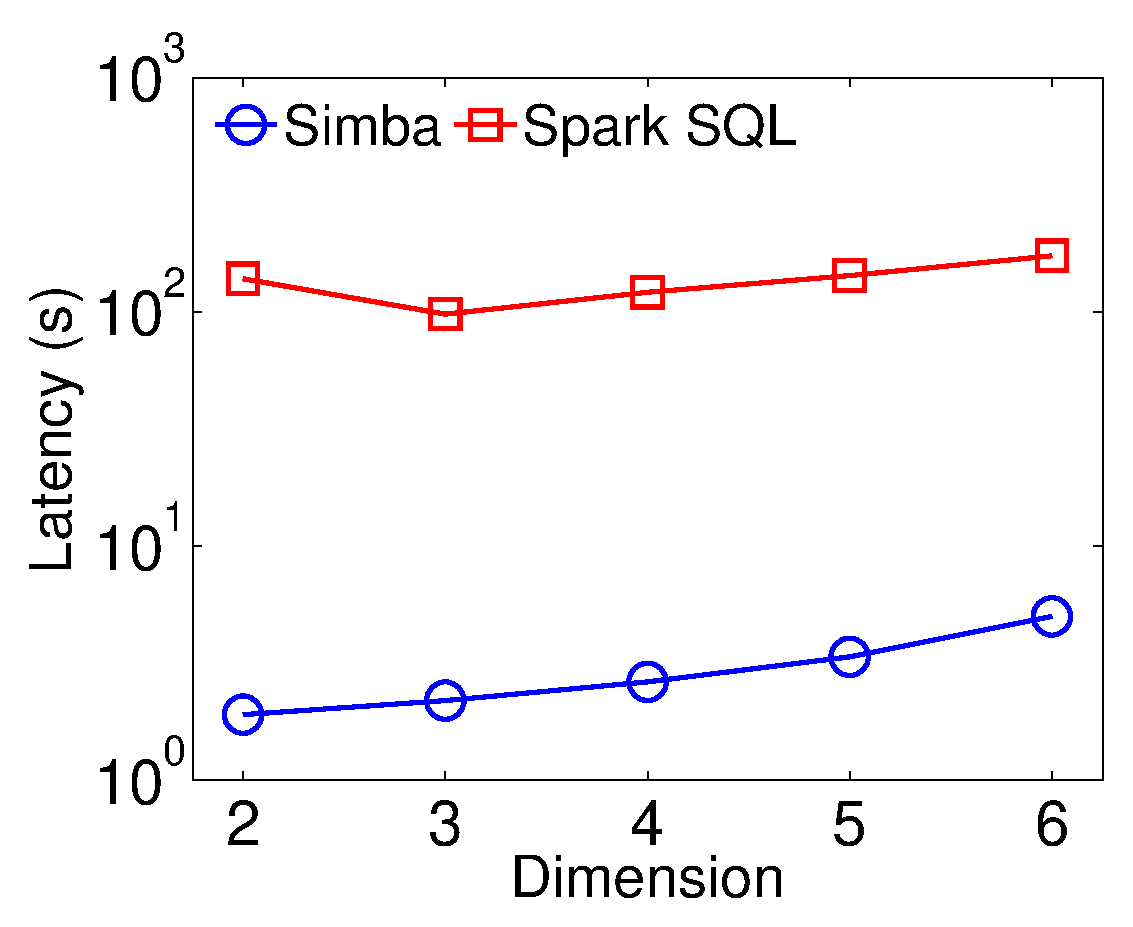
\includegraphics[width=1.55in]{figs/exp/gaussian700m_knn_dimension_latency}
	% }
	%\subfigure[GDELT]{
	%\label{fig:gdelt_knn_dimension}
	\subfigure[Throughput] {
		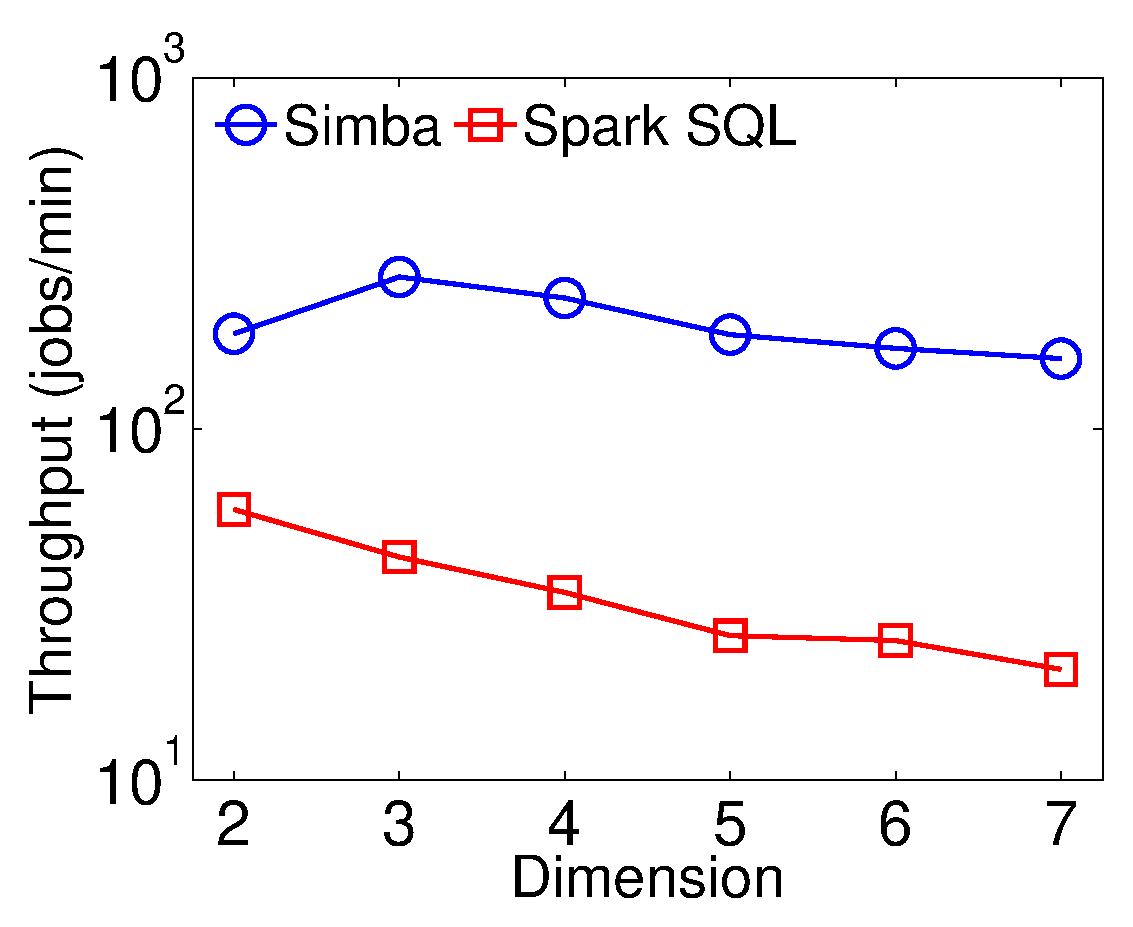
\includegraphics[width=1.55in]{figs/exp/gdelt_knn_dimension_throughput}
		\label{fig:gdelt_knn_dim_throughput}
	}
	\subfigure[Latency] {
		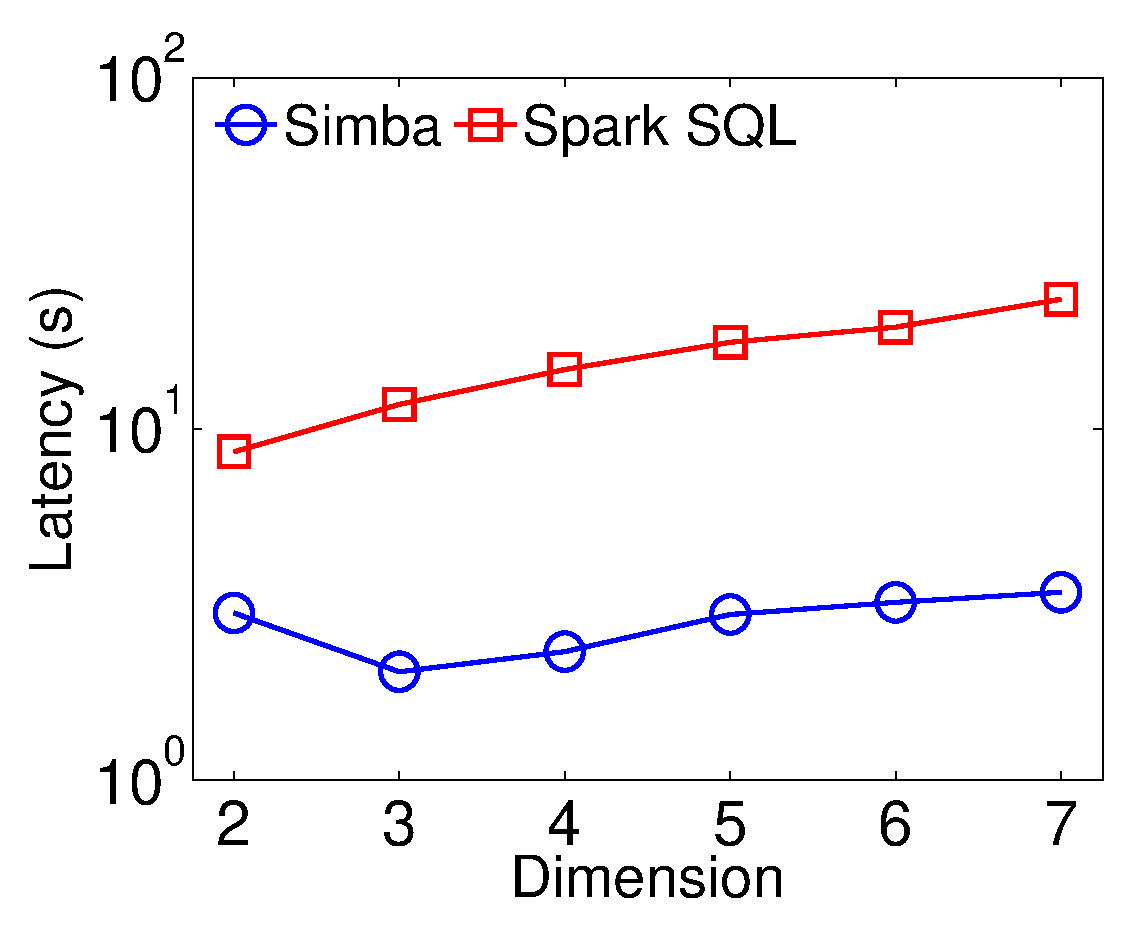
\includegraphics[width=1.55in]{figs/exp/gdelt_knn_dimension_latency}
		\label{fig:gdelt_knn_dim_latency}
	}
	%}\vspace{-1mm}
	\caption{\small $k$NN query performance vs. dimensionality on GDELT.}
	\label{fig:gdelt_knn_dimension}\vspace{-3mm}
\end{figure}

\begin{figure}[!t]
	\centering
	\subfigure[Distance join]{
		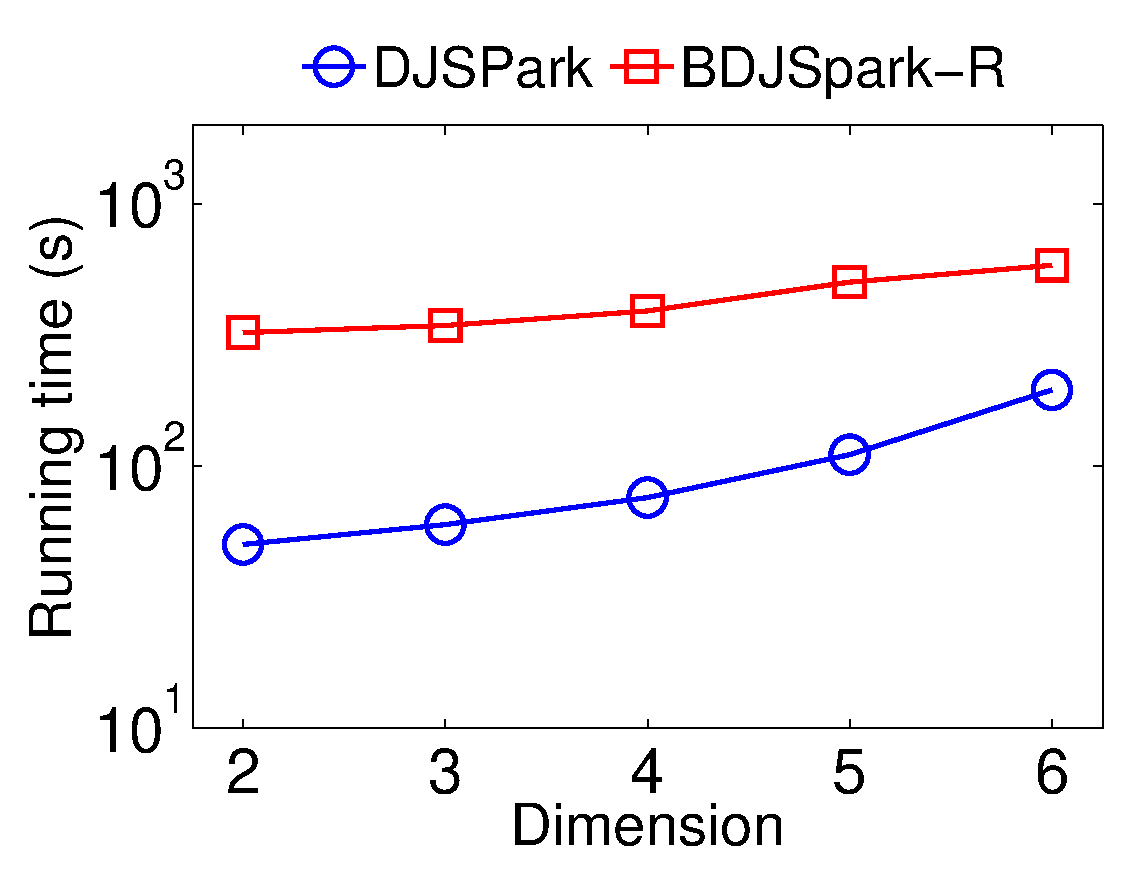
\includegraphics[width=1.55in]{figs/exp/osm_disj_dimension}
		\label{fig:synthetic_disj_dimension}}
	\subfigure[$k$NN join]{
		\includegraphics[width=1.55in]{figs/exp/osm_knnj_dimension}
		\label{fig:synthetic_knnj_dimension}}
	\caption{Join operations vs. dimensionality.}\vspace{-4mm}
	\label{fig:join_dim}
\end{figure}

\subsection{Support for Multi-Dimensions}
\label{sec:mdexp}
In this section, we evaluate the performance of \name and Spark SQL
when handling data in higher dimensions; note that other spatial
analytics systems, SpatialSpark, SpatialHadoop, and Hadoop GIS, {\em
  do not} support more than 2 dimensions.

For both range and $k$NN queries, as shown in Figures
\ref{fig:gdelt_rect_dimension} and \ref{fig:gdelt_knn_dimension}, both \name
and Spark SQL shows higher query latency and lower system throughput
using the GDELT data set, as dimensionality increases from $2$ to $6$.
But \name outperforms Spark SQL by 1-2 orders of magnitude in all cases.

% Figure \ref{fig:range_dim} shows how the number of dimensions
% influences range queries: On the synthetic RC dataset, \name and Spark
% SQL get slightly slower when the dimension number increases. On GDELT
% dataset, performance of \name is not stable since data distribution on
% different dimensions is not uniform. As to $k$NN queries shown in
% Figure \ref{fig:knn_dim}, performance on both data sets reduces
% steadily with the increasing of dimension number.  This is because the
% result sizes of $k$NN queries are fixed.


Figure \ref{fig:join_dim} shows the impact of dimensionality to the
join algorithms in \name, using two tables with 3 million records in
each table from the synthetic RC data set, when $d$ goes from $2$ to
$6$. The results show that the DJSpark and the RKJSpark algorithms
remain the best performance in all
dimensions. % From Figure \ref{fig:synthetic_disj_dimension}, we can observe
% that running time of BDJSpark-R grows slower than that of DJSpark and
% HDJSpark. The reason for this is the pruning power of the global join
% phase weakens with increasing of dimension number when the partition
% number is fixed. Similarly, BKJSpark-R grows slower than RKJSpark and
% VKJSpark (as shown in Figure \ref{fig:synthetic_knnj_dimension}) for
% the same reason. In addition, RKJSpark maintains comparable
% performance to VKJSpark on different dimension numbers.



%%% Local Variables:
%%% mode: latex
%%% TeX-master: "paper"
%%% End:

\section{Related Work}
\label{sec:related}
% Triggered by the needs on large-scale spatial data queries and analytics,
% there is an increasing interest in supporting spatial operations under
% distributed environment. Existing works can be classified as either efforts
% on supporting a specific spatial operation under a distributed computation
% framework (e.g. Hadoop) or a system designed for a suite of spatial operations.

\name is closely related to Spark and Spark SQL, which we have
reviewed in details in Section \ref{sec:background}. In particular,
\name has introduced many new components and significant extensions to
the Spark SQL core to build a full-fledged, native spatial query
engine over Spark. It adds spatial operators to both SQL and DataFrame
query interface, introduces indexing support over RDDs, designs and
implements novel spatial query algorithms and plans based on the RDD
abstraction and the new indexing support, and adds spatial-aware
optimizations to both the logical and physical optimizers as well as
exploring cost-based optimizations.

\dong{The last sentence of the first paragraph is too long and confusing.
It actually contains 4 `and's...}

In addition, spatial analytical systems running over a cluster are
also related, such as SpatialHadoop \cite{spatialhadoop} and Hadoop
GIS \cite{hadoopgis} that are based on Hadoop with the MapReduce
framework, which we have reviewed in Sections \ref{sec:background} and
\ref{sec:exp}. But since \name is based on Spark and Spark SQL which
explores in-memory computation using the RDD abstractions, the design
and system architecture are fundamentally different. As to Spark-based
systems like GeoSpark\cite{geospark} and SpatialSpark\cite{spatialspark},
they do not support (global and/or local) indexes natively over RDDs
as \name does. GeoSpark does not support spatial objects with additional
attributes (e.g. strings). None of Hadoop GIS, GeoSpark and SpatialSpark
provides a query engine like \name that supports SQL and DataFrame query
interfaces with query planning and optimization, except for SpatialHadoop
where a SQL-like query language called Pigeon (an extension of Pig\cite{pig})
is supported. Another important problem on such systems is that they
have to rely on user-level processes to support concurrent queries, which
greatly hurts system throughput. Performance-wise, \name has significantly
outperformed all these systems, including Spark SQL. 

Other than these systems, MD-HBase \cite{mdhbase} extends HBase to
support location services. It adds KD-tree and quad-tree indexes to
HBase to support range and $k$NN queries. GeoMesa \cite{geomesa}
builds a distributed spatial-temporal database on top of Apache
Accumulo \cite{accumulo}. It leverages GeoHash Index to provide
spatial queries over spatial-temporal data stored in Apache
Accumulo. Note that both HBase and Accumulo are both modeled after
Google's BigTable \cite{DBLP:journals/tocs/ChangDGHWBCFG08}, hence,
both MD-HBase and GeoMesa are essentially Key-Value stores with
support for spatial operations. As a result, both the design and the
objective of the system are very different from an in-memory spatial
analytical engine like \name, and the other systems we have examined
and compared with.

Most existing systems design indexing structures for the MapReduce
framework (e.g., Hadoop and HDFS), and they work with indexed data
from HDFS. In other words, they acquire data and indexes through a
distributed file system, which involves non-trivial disk
I/Os. SpatialSpark \cite{spatialspark} runs on top of Spark, but
rather than indexing RDDs natively, it partitions data, stores them
back to HDFS and {\em builds an index outside the Spark engine}.  An
open source project \cite{indexedrdd} provides an approach hat builds
index directly on Spark's RDD abstraction. However, it only supports
hash indexing on key-value pair RDDs, which doesn't extend to spatial
query processing and is very different from our indexing approach.

Other than these system efforts, indexing and query processing for
spatial data in the MapReduce framework have been explored by many
work in the literature, for example, z-value based indexing in
MapReduce \cite{cary2009experiences}, range queries in MapReduce
\cite{ma2009query, zhang2009spatial}, $k$NN queries in MapReduce
\cite{zhang2009spatial, akdogan2010voronoi}, $k$NN joins in MapReduce
\cite{feifeiknnj,bcknnj}, and spatial join over geometric objects in
MapReduce \cite{SJMR}. % In particular, using Hadoop . The SJMR
% algorithm \cite{SJMR} was proposed, which is a MapReduce version of
% the partition-based spatial-merge join (PBSM) algorithm \cite{pbsm}.
Note that a {\em distance join} $R \Join_{\tau} S$ can be converted
into a {\em spatial join} as we discussed in Section
\ref{sec:exp}. However, using a spatial join algorithm over this
mapping approach to solve distance join is not as efficient as solving
distance join over point objects directly, as geometric objects and
geometric relationships are in general much more expensive to deal. A
detailed review of spatial query processing in MapReduce is beyond the
scope of this paper, and we refer interested readers to the discussion
in \cite{spatialhadoop, hadoopgis} and references therein.

Lastly, various spatial partitioning strategies were explored in the
MapReduce framework using Hadoop. An extensive survey and performance
comparison of these results can be found in
\cite{sato,DBLP:journals/pvldb/EldawyAM15}. \name primarily explored
the Sort-Tile-Recursive (STR) partitioning scheme \cite{str} for its
indexing module, which has shown to be one of the best spatial
partitioning methods (e.g., see latest results in
\cite{DBLP:journals/pvldb/EldawyAM15}). That said, other spatial
partitioning methods can be easily employed and supported by \name,
and these results are orthogonal to the \name system.

% A method to construct R-Tree in Hadoop
% was proposed in \cite{cary2009experiences}, which partitions records
% according to their z-values, builds a separate R-tree for each
% partition and combines those R-trees under a common root.  Several
% solutions \cite{ma2009query, zhang2009spatial} was proposed to show
% how range queries can be handled with MapReduce, where the input file
% is scanned and each record is compared against the query range.  $k$NN
% queries in MapReduce is studied in \cite{zhang2009spatial} by taking a
% brute force approach that calculates the distance from the query point
% to each data point and then selects the data points with $k$ nearest
% distances. Another solution for $k$NN queries was proposed in
% \cite{akdogan2010voronoi}, which partitions data points using a
% Voronoi diagram and finds the answer in the partitions which is close
% to the query point. Besides, a MapReduce algorithm for reverse nearest
% neighbor (RNN) queries, which exploits the properties of Voronoi
% diagram, was proposed in the same paper \cite{akdogan2010voronoi}.

% As to processing $k$NN join under MapReduce framework, \cite{bcknnj}
% provides an algorithm leveraging Voronoi diagram based partition
% strategy, while \cite{feifeiknnj} proposes an approximate approach
% based on the properties of Z-values.


%Spatial join has been studied in MapReduce, in particular, using
%Hadoop \cite{SJMR}. The SJMR algorithm \cite{SJMR} was proposed which
%is a MapReduce version of the partition-based spatial-merge join
%(PBSM) algorithm \cite{pbsm}. Thus, a simple solution is to use the
%SJMR algorithm over the mapping approach above.
% SpatialHadoop adopts a two-level indexing strategy within the
% MapReduce framework so as to build and persist indexes for data stored
% in HDFS. \cite{sato} proposed an effective and scalable partitioning
% framework for Hadoop called SATO, which stands for four main steps in
% such framework: Sample, Analyze, Tear and Optimize. Hadoop-GIS makes
% use of this framework in building multi-level indexes. SpatialSpark
% partitions data stored on HDFS and builds a split-level global index
% with Apache Spark. Nevertheless, all solutions mentioned above
% requires pushing intermediate results and indexed data on HDFS. To
% make the matter worse, these systems have to acquire data and indexes
% through distributed file systems, which may bring non-trivial
% overheads of I/Os and API calls. An open source project
% \cite{indexedrdd} provides another approach that builds indexes upon
% Spark's RDD abstraction. However, it only supports hash indexing on
% key-value pair RDDs.



%%% Local Variables:
%%% mode: latex
%%% TeX-master: "paper"
%%% End:


\section{Conclusion}
\label{sec:conclude}
This paper introduces \name, a distributed in-memory spatial query and
analytical engine based on Spark. \name offers simple and expressive
query language in both SQL and DataFrame interfaces. It features low
query latency, high analytics throughput and excellent
scalability. \name extends Spark SQL with native support on a class of
common spatial operations, introduces indexes over RDDs, and adds
spatial-aware logical and cost-based optimizations that makes use of
existing indexes and statistics to select good query plans on the
fly. Extensive experiments conducted on large real data sets show
\name's superior performance against existing distributed spatial
query analytical engines and Spark SQL, and its support for
multidimensional data.

For future work, we plan to add native support on more geometric
objects (e.g., polygons) and additional spatial operators (e.g.,
spatial join over polygons) to \name. Efficient spatial operations on
very high dimensions and other metric spaces still present many
challenges. We also plan to design and implement more sophisticated
CBOs, such as using spatial histograms and kernel density estimate
(KDE), in \name for more effective autotuning.
 

%%% Local Variables:
%%% mode: latex
%%% TeX-master: "paper"
%%% End:



\small
\bibliographystyle{abbrv}
\bibliography{paper}
\normalsize
\begin{appendix}

\lstset{basicstyle=\small\ttfamily}

\section{\name Full Query Interface}
\label{sec:fullquery}
In this section, we list the full query interface for spatial operations and index
management in SQL query language and DataFrame API of \name.

\subsection{SQL Query Language}
\Paragraph{Points.} Users can use keyword \texttt{POINT} followed by a list of
expressions to express multi-dimensional points, where the number of expressions
indicates the number of dimensions. For example, we can use \texttt{Point(x - 1, y * 2)}
to express a two dimensional point with the value of $x - 1$ as the first dimension
and the value of $y * 2$ as the second dimension.

\Paragraph{Range predicates.} \name supports two different kinds of range queries:
box range queries and circle range queries. For box range queries, users should
use the following predicate to check if points are in the specific bounding box:
\begin{lstlisting}[language=SQL]
p IN RANGE(low, high)
\end{lstlisting}
In the predicate above, parameters \texttt{p}, \texttt{low} and \texttt{high}
should be point objects expressed by the grammar for points described above.
Specifically, \texttt{p} indicates the input point for predicate checking, while
\texttt{low} and \texttt{high} specify the bounding box.

Similarly, for circle range queries, users should use predicates as below:
\begin{lstlisting}[language=SQL]
p IN CIRCLERANGE(c, rd)
\end{lstlisting}
Note that \texttt{p} is the same as box range queries, while the point object
\texttt{c} and the constant \texttt{rd} indicates a circle centered at point
\texttt{c} with radius \texttt{rd} as the predicate area.

\Paragraph{$k$NN predicates.} Similar to range predicates, \name provides $k$NN
predicates as following:
\begin{lstlisting}[language=SQL]
p IN KNN(q, k)
\end{lstlisting}
It checks if \texttt{p} is in the $k$NN of point $q$ within the selection
domain. The selection domain is indicated by the relation after the same
level \texttt{WHERE} clause (when $k$NN predicates work as select conditions),
or the right-hand side relation of a $k$NN join operation (when $k$NN predicates
work as join conditions).

\Paragraph{Distance joins.} Users can use the SQL statement below to
express a distance join between two tables \texttt{R} and \texttt{S} with
distance threshold \texttt{rd}:
\begin{lstlisting}[language=SQL]
R DISTANCE JOIN S ON s IN CIRCLERANGE(r, rd)
\end{lstlisting}
Note that point \texttt{s} (resp. \texttt{r}) should be built from a record in
table $S$ (resp. $R$), or \name will be unable to resolve it.

\Paragraph{$k$NN joins.} A $k$NN join between table \texttt{R} and table \texttt{S}
can be expressed as following SQL statement:
\begin{lstlisting}[language=SQL]
R KNN JOIN S ON s IN KNN(r, k)
\end{lstlisting}
Similar to distance joins, $s$ (resp. $r$) should be built from a record in \texttt{S}
(resp. \texttt{R}). Users can also invoke an approximate $k$NN join using ZKJSpark
by replacing \texttt{KNN JOIN} by \texttt{ZKNN JOIN}.

\Paragraph{Index management.} \name allows users to manipulate indexes
easily with index management commands. Specifically, we can create
an index with the following command:
\begin{lstlisting}[language=SQL]
CREATE INDEX idx_name ON R(x, ...) USE idx_type
\end{lstlisting}
It builds a new index over a set of attributes in table \texttt{R} using the specific index
type (which can be R-tree, tree map or hash map), and names it as \texttt{idx\_name}.
We can check the built index on table \texttt{R} anytime using:
\begin{lstlisting}[language=SQL]
SHOW INDEX ON R
\end{lstlisting}
In addition, users can drop indexes by index names and/or table names using:
\begin{lstlisting}[language=SQL]
DROP INDEX idx_name ON table_name
DROP INDEX table_name
\end{lstlisting}

\subsection{DataFrame API}
\lstset{basicstyle=\scriptsize\ttfamily}
\Paragraph{Points.} We introduce point objects in DataFrame API, which wrap a list
of expressions into a multi-dimensional point that can be processed in \name. For
example, we can express a three dimensional point as following:
\begin{lstlisting}[language=java]
Point(tb("x"), tb("y"), tb("z"))
\end{lstlisting}
Specifically, the code above wraps three attributes \texttt{x}, \texttt{y} and \texttt{z}
from table \texttt{tb} into a point object for further processing.

\Paragraph{Single-relation operations.} Users can apply (box or circle) range queries
and $k$NN queries directly on data frames. Specifically, in DataFrame API, \name provides
following functions:
\begin{lstlisting}[language=java]
range(base: Point, low: Point, high: Point)
circleRange(base: Point, center: Point, r: Double)
knn(base: Point, q: Point, k: Int)
\end{lstlisting}
In the APIs described above, \texttt{base} indicates the point objects to be filtered,
while the other parameters give filter conditions.

\Paragraph{Join operaitons.} In the DataFrame API of \name, distance joins
and $k$NN joins can be expressed with following functions:
\begin{lstlisting}[language=java]
distanceJoin(other: DataFrame, left_key: Point,
             right_key: Point, rd: Double)
knnJoin(other: DataFrame, left_key: Point,
        right_key: Point, k: Int)
\end{lstlisting}
These functions will join the current data frame with another data frame \texttt{other}
on join conditions over \texttt{left\_key} and \texttt{right\_key}.

\Paragraph{Index management.} Users can easily create and drop indexes on data
frames with functions below:
\begin{lstlisting}[language=java]
index(index_type: IndexType, index_name: String, 
      attrs: Seq[Attribute])
dropIndex()
\end{lstlisting}

\setcounter{theorem}{0}
\section{Proof of Theorem 1}
\label{sec:proof1}
\begin{theorem}
For any partition $R_i$ where $i \in[1, n]$, we have:
\[\forall r \in R_i, \knn(r, S) \subset \{s|s \in S, |cr_i, s| \leq
\gamma_i\}, \textrm{ for }\gamma_i \textrm{ defined in
}\eqref{eq:rkjbound}.\]
\end{theorem}
\begin{proof}
Recall that $\knn(cr_i, S')=\{s_1, \ldots, s_k\}$ (in ascending
order of their distances to $cr_i$), and $u_i=\max_{r\in R_i}|r,
cr_i|$. Hence, for any $r \in R_i$, and for any $t \in [1, k]$, we
have:
\begin{align*}
|r, s_t|& \leq |r, cr_i| + |cr_i, s_t| \quad \textrm{(triangle inequality)}\\
   &\leq u_i + |cr_i, s_k|. \quad \textrm{(by construction)}
\end{align*}
This implies that a circle centered at $r$ with radius $(u_i + |cr_i,
s_k|)$ will cover at least $k$ points (i.e., at least $s_1, s_2, s_3,
.. s_k$) in $S'\subset S$. In other words, $\knn(r, S) \subset
S_r=\{s|s \in S, |r, s| \leq u_i + |cr_i, s_k|\}$. We denote this set
as the {\em cover set} of record $r$.

For each element $e \in S_r$, we have:
\begin{align*}
  |e, cr_i| & \leq |e, r| + |r, cr_i| \quad (\forall r\in R_i \textrm{, triangle inequality)} \\
  & \leq u_i + |cr_i, s_k| + u_i \\
  & = \gamma_i,
\end{align*}
 which implies $S_r$ is a subset
of $\{s|s \in S, |cr_i, s| \leq \gamma_i\}$.  Thus, $\forall r \in
R_i, \knn(r, S) \subset S_r \subset \{s|s \in S, |cr_i, s| \leq
\gamma_i\}.$
\end{proof}

\section{Additional Experiments}
\label{sec:addexp}
In this section, we show additional experiment results on how partition size influence
the performance of table indexing and different spatial operations in \name. Besides,
we present the influence of dimensionality on RC data sets for range and $k$NN queries
as well. 

\begin{figure}[!h]
	\centering
	% 	\includegraphics[width=1.55in]{figs/exp/osm_index_partsize_time}
	% 	\label{fig:index_partsize}}
	\includegraphics[width = 1.74in]{figs/exp/osm_index_partsize_time}\vspace{-4mm}
	\caption{Index construction cost: effect of partition size.}
	\label{fig:index_partsize}\vspace{-1mm}
\end{figure}

Figure \ref{fig:index_partsize} shows that its index construction cost
grows roughly linearly with respect to (wrt) partition size. This is
because it is more costly to build local indexes over larger
partitions (which outweighs the savings resulted from processing less
number of partitions). % Note that We only show results for
% \name since expected partition sizes for other systems are fixed to
% the HDFS block size.

\begin{figure}[!h]
	\centering
	\subfigure[Effect of partition size (number of records per partition).]{
		\label{fig:osm_rect_partsize}
		\includegraphics[width=1.55in]{figs/exp/osm_rect_partsize_throughput}
		\includegraphics[width=1.55in]{figs/exp/osm_rect_partsize_latency}
	}
	\caption{Range query performance on OSM: partition size.}
	\label{fig:rangepartition}\vspace{-1mm}
\end{figure}

Figure \ref{fig:rangepartition} shows the effect of partition size
(from $1 \times 10^5$ to $7 \times 10^5$ records per partition). As it
increases, the pruning power of global index in \name shrinks and so
does \name's performance. On the other hand, Spark SQL's performance
slightly increases as it requires fewer partitions to
process. Nevertheless, \name is still much more efficient due to its
local indexes and spatial query optimizer.

\begin{figure}[!h]
	\centering
	\subfigure[Effect of partition size (number of records per partition).]{
		\label{fig:osm_knn_partsize}
		\includegraphics[width=1.55in]{figs/exp/osm_knn_partsize_throughput}
		\includegraphics[width=1.55in]{figs/exp/osm_knn_partsize_latency}
	}\vspace{0mm}
	\caption{$k$NN query performance on OSM: partition size.}\vspace{-1mm}
	\label{fig:knnparition}
\end{figure}

In Figure \ref{fig:knnparition}, as the partition size increases,
the performance of \name decreases as the pruning power of global
index will drop when the partitions become larger.

Figure \ref{fig:osm_disj_partsize} shows the effect of partition size
on different distance join algorithms. As the partition size grows,
the running time of DJSpark and HDJSpark increases slightly, as the
pruning power of global join phase reduces when the partition
granularity is decreasing.  In contrast, BDJSpark-R becomes faster
because fewer local join tasks are required in the algorithm.

\begin{figure}[!h]
  \subfigure[Distance Join]{
		\label{fig:osm_disj_partsize}
		\includegraphics[width=1.55in]{figs/exp/osm_disj_partsize}
	} %\vspace{-6mm}
  \subfigure[$k$NN Join]{
    \label{fig:osm_knnj_partsize}
    \includegraphics[width=1.55in]{figs/exp/osm_knnj_partsize}
  }
	\caption{Effect of partition size for join operations.}\vspace{-2mm}
	\label{fig:partsize_on_join}
\end{figure}

Figure \ref{fig:osm_knnj_partsize} presents how partition size effect
the performance of different $k$NN join approaches. With the increase
of partition size, BKJSpark-R and RKJSpark grow faster since fewer
local join tasks are required for join processing. VKJSpark becomes
slightly slower as the partition size increases because the power of
its distance pruning bounds weakens when the number of pivots decreases.


\begin{figure}[h!]
	\centering
	\subfigure[Throughput] {
		\includegraphics[width=1.55in]{figs/exp/gaussian700m_rect_dimension_throughput}
		\label{fig:rc_rect_dim_throughput}
	}
	\subfigure[Latency] {
		\includegraphics[width=1.55in]{figs/exp/gaussian700m_rect_dimension_latency}
		\label{fig:rc_rect_dim_latency}
	}
	\caption{\small Range query performance vs. dimensionality on RC.}
	\label{fig:rc_rect_dimension} %\vspace{-2mm}
\end{figure}

\begin{figure}[h!]
	\centering
	\subfigure[Throughput] {
		\includegraphics[width=1.55in]{figs/exp/gaussian700m_knn_dimension_throughput}
		\label{fig:rc_knn_dim_throughput}
	}
	\subfigure[Latency] {
		\includegraphics[width=1.55in]{figs/exp/gaussian700m_knn_dimension_latency}
		\label{fig:rc_knn_dim_latency}
	}
	\caption{\small $k$NN query performance vs. dimensionality on RC.}
	\label{fig:rc_knn_dimension} %\vspace{-2mm}
\end{figure}
Lastly, Figures \ref{fig:rc_rect_dimension} and \ref{fig:rc_knn_dimension}
show the results for range and $k$NN queries when dimensionality
increases from $2$ to $6$, using the synthetic RC data set. The
results show similar trends to that on the GEDLT dat set as in Figures
\ref{fig:gdelt_rect_dimension} and \ref{fig:gdelt_knn_dimension}: \name has significantly
outformed Spark SQL in all dimensions.

\end{appendix}
%%% Local Variables:
%%% mode: latex
%%% TeX-master: "paper"
%%% End:


\end{document}
